% == DOCUMENT HEADER == 
\documentclass[czech, bc, kiv, he, iso690numb, pdf]{fasthesis}

% == PACKAGES AND SETTINGS ==
\usepackage{multirow}
\usepackage{ragged2e}
\usepackage{tikz}
\usepackage{pdflscape}
\usepackage{rotating}
\usepackage{pdfpages}
\usepackage{booktabs}
\usepackage{svg}

\usetikzlibrary{positioning}
\newlength{\pipeNodeW}

\lstdefinestyle{plain}{
	%basicstyle=\ttfamily\footnotesize,
	style=FASThesisLstStyle,
    %backgroundcolor=\color{FASThesis@UWBGray!25},
    numberstyle=\tiny\color{gray},
	numbers=none,
	numbersep=5pt,
	keepspaces=true,
	tabsize=5,
	columns=fullflexible,
	extendedchars=true,
    numberblanklines=false,
	literate={á}{{\'a}}1 {č}{{\v{c}}}1 {ď}{{\v{d}}}1 {é}{{\'e}}1 {ě}{{\v{e}}}1 {è}{{\`{e}}}1 {í}{{\'{\i}}}1 {ľ}{{\v{l}}}1 {ň}{{\v{n}}}1 {ó}{{\'o}}1 {ŕ}{{\'r}}1 {ř}{{\v{r}}}1 {š}{{\v{s}}}1 {ť}{{\v{t}}}1 {ú}{{\'u}}1 {ů}{{\r{u}}}1 {ý}{{\'y}}1 {ž}{{\v{z}}}1
	{Á}{{\'A}}1 {Č}{{\v{C}}}1 {Ď}{{\v{D}}}1 {É}{{\'E}}1 {Ě}{{\v{E}}}1 {È}{{\`{E}}}1 {Í}{{\'I}}1 {Ľ}{{\v{L}}}1 {Ň}{{\v{N}}}1 {Ó}{{\'O}}1 {Ŕ}{{\'R}}1 {Ř}{{\v{R}}}1 {Š}{{\v{S}}}1 {Ť}{{\v{T}}}1 {Ú}{{\'U}}1 {Ů}{{\r{U}}}1 {Ý}{{\'Y}}1 {Ž}{{\v{Z}}}1
	{--}{{--}}1 {-}{{-}}1
}

\lstdefinestyle{json}{
    style=plain,
    numbers=left
}

\newcommand{\nobreakstart}
{
    \nopagebreak
    \begin{center}
        \begin{minipage}{\textwidth}  
}

\newcommand{\nobreakend}{
        \end{minipage}
    \end{center}
}



\title{Vyhodnocení schopnosti LLM analyzovat projektovou dokumentaci a těžit z~ní klíčové parametry}
\author{Daniel}{Sibolerski}{}{}
\supervisor{Ing. Richard Lipka, Ph.D.}
\stagworkid{104281}
\assignment{res/zadani.pdf}
%\signdate{31}{12}{2024}{V Nové Vsi u~Nového Města na Moravě}
\addbibresource{res/references.bib}


% == DOCUMENT FRONTMATTER TEXTS ==
\abstract{Tato bakalářská práce se zabývá zkoumáním schopnosti velkých jazykových modelů extrahovat a formalizovat informace ze specifikací požadavků na software psaných v~přirozeném jazyce. Využitím long context přístupu je zaručeno, že jazykový model dostane na vstupu celý dokument a může v~něm vyhledávat potřebné požadavky. Pro tento úkol byl vyvinut nástroj, který tyto dokumenty načte, zpracuje, odešle do velkého jazykového modelu a umožní uživateli výsledky analyzovat a zkontrolovat.}{This bachelor thesis investigates the ability of large language models to extract and formalize information from software requirement specifications written in natural language. Long context approach ensures that model processes the whole document and is able to search specified requirements in it. A~tool was developed for this task, which loads given documents, stores them in a database, sends them to the model and allows the user to check and validate its outputs.}
\keywords{LLM, velký jazykový model, extrakce, formalizace, analýza, SRS, specifikace softwarových požadavků}

% == ACKNOWLEDGEMENT ==
\acknowledgement{Děkuji Ing. Richardu Lipkovi, Ph.D. za nápad na tuto bakalářskou práci, jeho pomoc a vstřícnost. Každá jeho rada byla velmi přínosná a přispěla k~zisku potřebných znalostí a nápadů na tvorbu.}

% == ADDITIONAL FRONT MATTER CONTENT ==
% \auxfrontmattercontent{%
% \section*{...}
% \fbox{\parbox[t]{\textwidth}{\textbf{%
% ...
% }}}}

% == DOCUMENT TEXT == 
\begin{document}
\frontpages[tm]
\tableofcontents

%\chapter*[Předmluva]{Předmluva}
%...

% =================================================================================
\chapter{Úvod}
Součástí dodávky software je specifikace požadavků na software (SRS), ve které je nutné definovat potřeby kladené na systém. Tyto specifikace jsou závazné a při jejich nesplnění je nutné software upravit, což je ekonomicky náročné. Jedna specifikace může mít desítky až stovky stran a obsahovat stovky požadavků, jejichž ruční nalezení zabere velké množství času. Je také potřeba sledovat, zda byly v~průběhu vývoje tyto požadavky naplněny, proto by měly být uloženy v~databázi, což proces vývoje zjednoduší. Automatizace tohoto procesu navíc snižuje riziko přehlédnutých nebo zapomenutých požadavků. Velké jazykové modely (LLM) přinesly možnost automaticky prohledávat tyto dokumenty a extrahovat z~nich potřebné informace. Cílem této práce je proto prozkoumat možnosti, které tyto velké jazykové modely přinášejí, a zjistit, zda jsou pro tento úkol vhodné.

Nástroj pro extrakci softwarových požadavků využívá přístupu dlouhého kontextu (long context), kde má daný model dostupný celý dokument a je mu umožněno v~něm vyhledávat. Nástroj je rozdělen na dvě části -- extrakční a formalizační. Extrakční část umožňuje LLM vyhledávat v~celém dokumentu potřebné požadavky definované uživatelem. Ve formalizační části model z~těchto extrahovaných požadavků vytváří strukturovaný výstup, čímž je možné získat specifické informace z~kratšího textu.

Výstupy z~LLM je potřeba porovnat s~ruční extrakcí a formalizací, která byla provedena na dvou dokumentech. Pro toto porovnání bylo vyvinuto grafické uživatelské rozhraní, které umožňuje v~extrakční části porovnat ručně extrahované požadavky s~výstupy z~LLM. Ve formalizační části je pak umožněno porovnat strukturovaný požadavek s~referenčními formalizacemi.

S~výsledky hodnocení je možné vypočítat evaluační metriky. Pro extrakční část jsou to precision, recall a F1 skóre a pro formalizační část accuracy. Díky nim je možné zjistit, zda jsou LLM schopny tento úkol splnit a ušetřit tak lidem práci s~vyhledáváním, formalizací a evidencí požadavků.
 
% =================================================================================
% Seznamnte se s problematikou extrakce dat z textů v přirozeném jazyce.
% =================================================================================
\chapter{Možnosti extrakce informací}
V~současné době existuje více informací v~elektronické podobě, než v~papírové \cite{information-extraction}. To, že jsou digitalizované, z~nich dělá informace, ve kterých se dá vyhledávat a těžit z~nich klíčové parametry automatizovaně. Problém je, že většina explicitních informací je uložena v~nestrukturovaných systémech (například na disku v~nestrukturovaných dokumentech), než ve strukturovaných (třeba v~databázích, které umožňují jednoduše vyhledávat a filtrovat).

Extrakce informací z~textu je tedy technika zpracování přirozeného jazyka, jejímž cílem je vypsat strukturovaná data z~nestrukturovaného, případně polostrukturovaného textu \cite{llm-with-nlp-long-docs-info-extraction}. V~současné době existuje mnoho způsobů, jak extrakce informací docílit. Některé z~nich jsou založeny na regulárních výrazech, jiné využívají strojové učení nebo kombinaci obojího. V~této kapitole jsou popsány některé z~těchto metod pro zpracování přirozeného jazyka.

Cowie a Lenhert \cite{information-extraction} popisují informační extrakci (IE) jako technologii, která transformuje nestrukturovaná textová data do strukturovaného, strojově čitelného formátu, čímž řeší problém informačního přetížení. IE doplňuje a rozšiřuje možnosti tradičních systémů pro vyhledávání informací (Information Retrieval, IR). Zatímco IR systémy fungují jako nástroje, které z~rozsáhlých textových dat shromažďují potenciálně užitečný materiál, IE systémy tento surový materiál dále zpracovávají a redukují na klíčovou esenci původního textu.


\section{Historie}
Článek \cite{information-extraction} popisuje kořeny IE sahající před rok 1970, ale hlavní rozdíl mezi ranými systémy a systémy z~90. let spočíval v~dostupnosti rozsáhlých testovacích korpusů s~anotovanými \uv{správnými odpověďmi} (šablonami), které umožnily systematické hodnocení a vývoj.

\subsection{Klíčové iniciativy}
Klíčové iniciativy (popsané v~článku \cite{information-extraction}) MUC (Message Understanding Conferences)  a program Tipster, financované americkou vládou (konkrétně agenturou DARPA/ARPA), zásadním způsobem formovaly a urychlily vývoj technologií pro extrakci informací. % Tyto projekty poskytly výzkumné komunitě společná data, definované úkoly a standardizované metody hodnocení, což umožnilo objektivní srovnání různých systémů.
Konference MUC sloužily jako soutěžní a evaluační platforma pro systémy zpracování přirozeného jazyka. Jejich hlavním účelem bylo posunout výzkum od malých systémů a umělých dat k~velkým systémům pracujícím s~reálným jazykem. %\cite{information-extraction}.
První dvě konference (MUCK-1 v~roce 1987 a MUCK-2 v~roce 1989) se zaměřovaly na extrakci informací z~malého počtu krátkých námořních zpráv. (Písmeno \uv{K} z~akronymu bylo později vypuštěno). MUC-3 (1991) a MUC-4 (1992) přinesly změnu tématu a typu textu. Úkolem bylo zpracovat texty z~novin a zpravodajských agentur týkající se teroristických incidentů v~Latinské Americe. Účastníci obdrželi sadu trénovacích textů a k~nim příslušné vyplněné šablony (templates). Při samotném hodnocení musely jejich systémy zpracovat novou sadu textů a automaticky vyplnit šablony, které byly následně skórovány oproti správným odpověďím (klíčům) -- průběh skórování byl vyhodnocen nezávislou skupinou. Pravidelná setkání umožnila výzkumným týmům sdílet poznatky, což vedlo k~rychlému osvojení úspěšných technik napříč komunitou. %, jako bylo například částečná syntaktická analýza (partial parsing) místo snahy o kompletní větný rozbor.

Iniciativa Tipster, zahájená v~reakci na pokrok v~MUC-3, měla širší záběr. Jejím cílem bylo kombinovat technologie vyhledávání informací (IR) a extrakce informací (IE) a kladla důraz na přenositelnost a rekonfigurovatelnost systémů. Na rozdíl od úzce zaměřených MUC se Tipster soustředil na dvě odlišné oblasti:
\begin{itemize}
    \item \uv{joint ventures} (obchodní dohody),
    \item výroba mikroelektroniky (technické texty), dále vyžadoval funkčnost ve dvou jazycích -- angličtině a japonštině.
\end{itemize}

\section{Digitalizace papírových informací}
Pro tvorbu strojově čitelného textu z~papírových informací lze použít například techniku OCR (optic character recognition), kterou shrnuje článek \cite{ocr}. Tato technika vznikla již v~50. letech 20. století. Jedná se o~optické zpracování textu a jeho převedení do podoby, ve které se dá strojově zpracovat. Papírový dokument se nejprve naskenuje a dále se na něj aplikují různé metody, jako například:
\begin{itemize}
    \item porovnání s~předdefinovanou šablonou,
    \item rozpoznání strukturálních vzorů (což nemusí fungovat pro ručně psané texty),
    \item neuronové sítě (konvoluční, rekurentní).
\end{itemize} 

Neuronové sítě v~tomto odvětví dosahují nejlepších výsledků, někdy přesnosti i více než 99 \%.

\section{Regulární výrazy}
Regulární výrazy jsou sekvence znaků, které definují vzor pro vyhledávání entit v~textu. Jako entita je považována textová informace, která odpovídá jasnému formátu -- jde například o~telefonní čísla, e-mailové adresy nebo datumy \cite{regex-learning-for-info-extraction}.

Pro pevně daný formát textu jsou regulární výrazy velmi efektivní a rychlou metodou pro extrakci dat, avšak nedokážou zachytit hlubší kontext z~textů. Jejich použití je proto omezené na specifický případ, zejména semistrukturovaný text nebo text s~jasně definovanými vzory. Takovým případem jsou například programovací jazyky, které mají pevně danou syntaxi a je tak možné na ně aplikovat regulární výrazy \cite{regular-expressions-oop}. Znaky pro tvorbu regulárního výrazu se však mohou lišit pro danou oblast/programovací jazyk.

Článek \cite{regex-relation-clinical} popisuje konkrétní možnost nalezení relací (implementovanou v~jazyce \product{Python}) v~klinických textech, které obsahují nestrukturovaná nebo semistrukturovaná data. Je tím docíleno použitím takového výrazu, který dokáže najít konkrétní vyhledávaný text a případně jeho okolí -- následující slovo, řádek nebo celý odstavec.

\section{Vývoj jazykových modelů}
Pravděpodobně první člověk, který začal studovat jazykové modely, byl Andrey Markov \cite{llm-past-present-future}, \cite{first-links-markov-chain}. V~roce 1906 představil Markov svůj první model, dnes nazývaný \textbf{Markovův řetězec}, se dvěma stavy a pravděpodobnostmi přechodu z~jednoho stavu do druhého. Konkrétně v~roce 1913 toto aplikoval na román Evžen Oněgin, kde z~prvních 20 000 znaků odstranil mezery a interpunkci, rozdělil ho na souhlásky a samohlásky a spočítal pravděpodobnosti přechodů mezi nimi. Na těchto datech pak ověřil, že při těchto přechodech mezi stavy podle těchto pravděpodobností se frekvence výskytu stavů časem ustálí na určitých hodnotách odpovídajících očekávaným pravděpodobnostem.\footnote{Pro toto ustálení pravděpodobností musí platit podmínka ergodicity a stacionarity.} Později toto tvrzení zobecnil a dokázal pro libovolný počet stavů \cite{llm-past-present-future}. %Podle Shannon-McMillan-Breiman teorému musí pro být toto ustálení pravděpodobností splněn předpoklad ergodicity a stacionarity.

Z~tohoto modelu vychází \term{n-gramové modely}, které říkají, že pravděpodobnost výskytu určité sekvence znaků závisí pouze na předchozích $n$-1 slovech v~sekvenci -- tzv. \textbf{Markovské modely řádu ($n$-1)} \cite{llm-past-present-future}.

\subsection{N-gram}
Jakýkoliv text lze rozdělit na menší části, které se nazývají $n$-gramy. To jsou sekvence $n$ po sobě jdoucích položek (slov nebo znaků) z~daného textu \cite{n-grams}.

Podle \cite{n-grams} jsou jazykové modely formálně jen statistické rozdělení $n$-gramů (nebo sekvence slov), které předpovídají pravděpodobnost výskytu dalšího slova na základě předchozích slov. Používá tedy historii $n-1$ bezprostředně předcházejících slov, kde $n$ je počet slov, k~předpovědi pravděpodobnosti $P$ výskytu dalšího slova. 

Příkladem takového využití pravděpodobností výskytů slov je \product{Chomsky bot} \cite{chomskybot}, který generuje věty na základě pravděpodobnostního modelu z~$n$-gramů vytvořeného z~textů Noama Chomského\footnote{Noam Chomsky je americký filozof, kognitivní vědec a mimo jiné tvůrce Chomského hierarchistické klasifikace formálních jazyků \cite{chomsky-wiki} \cite{llm-past-present-future}.}.

\subsection{Neuronové jazykové modely}
V~roce 2003 přinesly \textbf{neuronové jazykové modely} (neural language models) \cite{neural-probabilistic-lm} významný pokrok v~oblasti zpracování přirozeného jazyka. Ty vylepšily $n$-gramové modely tím, že zavedly \textbf{word embedding}, což jsou vektory reálných čísel, které efektivněji reprezentují slova nebo sousloví. Dalším výrazným vylepšením $n$-gra\-mových modelů byla reprezentace jazykového modelu \textbf{neuronovou sítí}, což snížilo počet parametrů modelu.

Dále byly vyvinuty rekurentní neuronové sítě (RNN), včetně long-short-term-memory (LSTM) \cite{llm-past-present-future}, které umožnily modelům zachytit dlouhodobé závislosti v~textu. 

LSTM modely byly schopny efektivněji zpracovávat dlouhé sekvence textu a generovat koherentnější výstupy při tréninku na velkém množství dat \cite{llm-past-present-future}.

\subsection{Transformer modely}
Zásadní pokrok přišel s~představením \textbf{transformer} architektury \cite{llm-past-present-future} v~roce 2017 od společnosti Google \cite{attention-is-all-you-need}, \cite{great-transformer}. Transformer modely využívají mechanismus sebepozornosti (self-attention), který umožňuje modelu zaměřit se na různé části vstupní sekvence při generování výstupu. Tento přístup umožnil paralelní zpracování dat \cite{great-transformer}, což výrazně zrychlilo trénink a zlepšilo schopnost modelu zachytit dlouhodobé závislosti v~textu \cite{llm-past-present-future}. Tyto modely se staly základem pro mnoho moderních velkých jazykových modelů, jako je GPT (Generative Pre-trained Transformer) od OpenAI nebo BERT od Google \cite{great-transformer}.



%=================================================================================
% Seznamte se s dostupnými LLM a postupy jejich využití pro zpracování technických textů.
%=================================================================================
\chapter{Velké jazykové modely}
V~posledních letech se velké jazykové modely (LLM) staly populárním nástrojem pro zpracování přirozeného jazyka. Takové modely jsou trénovány na velkém množství textových dat a jsou schopny generovat text, odpovídat na otázky a komunikovat v~přirozeném jazyce s~velkou přesností \cite{chat-gpt-llm-education}. 

Pro zpracování přirozeného jazyka je v~současnosti dostupných mnoho velkých jazykových modelů, které lze použít pro různé úkoly, včetně extrakce informací z~textu. Mezi nejznámější firmy vyrábějící jazykové modely patří například OpenAI, Mistral nebo Meta. Tyto společnosti vyvinuly různé modely s~různými schopnostmi a vlastnostmi, které jsou vhodné pro různé aplikace a nabízejí různé přístupy k~využití těchto modelů.

Tyto firmy nabízí pro uživatele přístup k~těmto modelům \textbf{prostřednictvím API}, které umožňuje integraci těchto modelů do různých aplikací a služeb. Uživatelé mohou tyto modely využívat k~různým účelům díky generování textu -- odpovídání na otázky, tvorba kódu, strukturovaných dat a další.

\section{Modely od OpenAI}
Společnost OpenAI v~současnosti nabízí několik velkých jazykových modelů, které jsou široce používány pro různé úkoly zpracování přirozeného jazyka. Mezi nejznámější patří řada GPT (Generative Pre-trained Transformer) modelů, které jsou schopny generovat text, odpovídat na otázky a provádět různé další úkoly. Tyto sekce vycházejí z~oficiální dokumentace OpenAI \cite{openai-platform-models}, kde jsou detailně popsány dostupné modely a jejich vlastnosti.

Každý model je navržen pro různé účely a má různé schopnosti. Pro řešení komplexních úloh, jako například složitých matematických úloh, jsou vhodné modely disponující \textbf{uvažováním (reasoning)}. Uvažování umožňuje modelu se \uv{zamyslet} nad problémem před tím, než poskytne odpověď (více popsáno v~sekci \ref{sec:reasoning}) -- generuje myšlenkové pochody, díky kterým si vlastně \textit{buduje cestu k~výsledku}. Dá se to ilustrovat například na matematických operacích, které se dají těžko vypočítat v~hlavě zpaměti. Avšak, pokud se model nad odpovědí \uv{zamyslí} a napíše si postup, je větší pravděpodobnost, že výsledek bude přesnější. Pro tento účel (uvažování) je vhodné využít \textbf{Responses API}, které je na toto chování určeno.

\textbf{Responses API} je nová verze pro \textbf{Chat Completions API}, která je optimalizována pro generování delších a komplexnějších odpovědí. Tento koncový bod API je navržen tak, aby lépe zvládal úkoly vyžadující uvažování, jako jsou matematické výpočty, logické dedukce a další složité operace. OpenAI \cite{openai-platform-migrate-responses} doporučuje pro nové aplikace využívat právě \textbf{Responses API} kvůli lepšímu výkonu, lepší dostupnosti v~budoucnosti a zmenšeným nákladům, které jsou o~40~\% až 80~\% nižší než u~předchozího \textbf{Chat Completions API} díky použití mezipaměti (\texttt{cache}).

\subsection{Strukturovaný výstup}
Modely od společnosti OpenAI umožňují generovat strukturované výstupy \cite{openai-structured} podle zadaného \verb"JSON" schématu. Stačí modelu při tvorbě požadavku přidat schéma (například vlastní třídu dědící od \verb"BaseModel" z~knihovny \product{pydantic} \cite{pydantic}). Model poté vždy vygeneruje odpověď, která odpovídá tomuto schématu, kde jsou vyplněné potřebné atributy.

\section{Modely od Meta}
Některé modely od společnosti Meta jsou \textbf{volně dostupné} a dají se spustit lokálně na osobním počítači. Je důležitá velikost tohoto modelu, protože při potřebě spustit model lokálně je potřeba dostatečné množství operační paměti, do které se model musí nahrát. Rychlost paměti také závisí na rychlosti generovaných odpovědí, velikost modelu (a počet parametrů) závisí na kvalitě výstupů.

Služba \product{Ollama} nabízí rozhraní pro spouštění lokálních jazykových modelů, například \verb"llama3.2:latest" \cite{llm-llama}. Tento model (upravený a připravený pro lokální spuštění) má velikost \verb"2 GB" a jeho kontextové okno je 128 000 tokenů. Díky knihovně \product{ollama} pro jazyk \product{Python} lze potom s~modelem komunikovat přes rozhraní API, pokud je model spuštěný lokálně.

\product{Ollama} také nabízí strukturované výstupy v~modelu podle zadaného schématu \cite{ollama-structured}.

\section{Modely od Mistral}\label{sec:modely-od-mistral}
Jazykové modely společnosti Mistral se dají rozdělit do tří hlavních skupin -- Mistral Small, Mistral Medium a Mistral Large.

Od každé kategorie se modely číslují chronologicky podle verze vydání. Všechny tyto modely také umožňují při použití API generovat výstupy v~dané struktuře \cite{mistral-structured}. Tyto modely se liší ve velikosti, tedy počtu parametrů a vah, na kterých byly trénovány.

Výstup z~LLM \textbf{není deterministický}, avšak pro API použitých modelů (nejen od Mistral) existuje atribut \verb"temperature". Ten umožňuje předat číslo, které určuje míru náhodnosti. Při použití menšího čísla je výstup více deterministický, naopak s~větším číslem více kreativní \cite{mistral-temperature}.

\section{Rozdíly mezi modely}
Každý velký jazykový model má různé vlastnosti, které definují jeho chování a odpovědi. Může to být například různými trénovacími daty, velikostí modelu nebo velikostí kontextového okna modelu. Následující sekce popisují hlavní rozdíly mezi velkými jazykovými modely.

\subsection{Kontextové okno}
Každý velký jazykový model má schopnost udržovat si \textbf{po nějakou dobu} informace o~probíhající konverzaci a jejím \textbf{kontextu}. Z~toho vyplývá, že každý model má vlastní \term{kontextové okno} pro každou konverzaci. Anthropic \cite{claude-platform-context-windows} ve své dokumentaci definuje kontextové okno jako množství textu, na které jazykový model může odkazovat a které může sledovat při generování nového textu, plus vygenerovaný text. Nechť velikost kontextového okna je $K$, vstup/zpráva uživatele je $M_{in}$ a textový výstup vygenerovaný jazykovým modelem je označen $M_{out}$. V~každém odeslání zprávy je tedy jazykovému modelu poslán text $T$. Při posílání $j$ promptů jazykovému modelu platí tedy rovnice ve vzorcích \ref{eq:kontext_t1} a \ref{eq:kontext_tj}.

\begin{eqnarray}
    T_1 & = & M_{{in}_1} + M_{{out}_1} \label{eq:kontext_t1} \\
    T_{j,\ j\ >\ 1} & = & T_{j-1} + M_{{in}_j} + M_{{out}_j} \label{eq:kontext_tj}   
\end{eqnarray}

Je zřejmé, že suma všech textů $T$ musí být menší nebo rovna než velikost kontextového okna $K$ (vzorec \ref{eq:kontext_velikost}), aby model chápal původní smysl konverzace.

\begin{equation}
    \label{eq:kontext_velikost}
    \sum_{i=1}^{j} T_i \leq K
\end{equation}

\subsection{Schopnost uvažování v~modelech}\label{sec:reasoning}
Článek \cite{llm-gpt-reasoning} popisuje schopnost GPT modelů provádět \term{uvažování}\footnote{označením \uv{uvažování} u~LLM není myšleno  lidské přemýšlení, ale schopnost rozdělit úkol na menší části v~důsledku dopracování se k~lepšímu výsledku} pomocí techniky zvané \textbf{Chain-of-Thought (CoT) prompting}. Tato technika zahrnuje poskytování příkladů modelu, které ukazují krok za krokem myšlenkový proces potřebný k~dosažení správné odpovědi na komplexní otázky. Tímto způsobem se model učí generovat podobné myšlenkové pochody pro nové otázky, což vede k~lepším výsledkům při řešení problémů vyžadujících uvažování.

Tato studie \cite{llm-gpt-reasoning} rozlišuje dva systémy usuzování -- \textbf{systém 1} a \textbf{systém 2}. Systém 1 je rychlý, automatický a intuitivní, který často využívá zkratky, což může vést k~chybám. Systém 2 je naopak pomalý, uvážlivý a logický, což vyžaduje vědomé úsilí. Autoři poznamenávají, že LLM se na první pohled jeví jako myslitelé Systému 1, protože generují text automaticky slovo po slově na základě pravděpodobnosti. Nicméně modely mohou simulovat procesy Systému 2 tím, že využívají své kontextové okno jako externí krátkodobou paměť pro \textbf{chain-of-thought} (řetězec myšlenek) -- tedy postupné logické kroky, které jim umožňují řešit složitější problémy podobně, jako když si lidé dělají poznámky.

Z~výzkumu vyplynulo, že použití \textbf{chain-of-thought prompting} výrazně zlepšuje schopnost modelů řešit problémy vyžadující uvažování, jako jsou matematické úlohy, logické dedukce a další komplexní úkoly. Autoři také zjistili, že novější modely mají tendenci lépe využívat tuto techniku (například \verb"ChatGPT-4"), oproti starším modelům (jako \verb"GPT-3"), což naznačuje, že schopnost uvažování se zlepšuje s~vývojem modelů. U~starších modelů byla snaha o~\uv{vynucení} uvažování tím, že se na konec promptu přidal text s~instrukcí o~zavedení přemýšlecího procesu, například \uv{Použij algebru.}. Každopádně, podle výzkumu novější modely již tento přístup nepotřebují, ale spustí CoT i přes to, že na konci promptu je výslovná žádost o~krátkou odpověď. To je přisuzováno tomu, že novější modely byly trénovány na větším množství dat a mají lepší intuitivní schopnosti.

% Anthropic -- Faithfulness of Reasoning in LLMs
Studie \cite{anthropic-reasoning-paper} zkoumala \textbf{věrnost a nevěrnost CoT} vybraných modelů se schopností uvažovat (\verb"Claude 3.7 Sonnet", \verb"DeepSeek R1") a modelů bez schopnosti uvažovat (\verb"Claude 3.5 Sonnet", \verb"DeepSeek V3"). Pro měření věrnosti (\uv{faithfulness}) \\ myšlenkových procesů (CoT) autoři použili dvojice promptů: standardní otázku a tutéž otázku s~vloženou nápovědou (\uv{hint}), která směrovala k~určité odpovědi. Pokud model změnil svou odpověď na základě nápovědy, výzkumníci analyzovali jeho CoT. Za \verb"věrný" byl označen pouze ten CoT, u~kterého model explicitně přiznal, že nápovědu použil. Pokud nápovědu využil, ale v~myšlenkovém řetězci ji zamlčel, byl vyhodnocen jako nevěrný.

Autoři provedli vlastní fine-tuning, tedy dotrénování, modelu \\ \verb"Claude 3.7 Sonnet" pomocí outcome-based Reinforcement Learning (RL) (učení posilováním založené na výsledcích) v~syntetických prostředích. Záměrně nastavili systém odměn tak, aby model získal $+1$ bod za výběr fakticky nesprávné odpovědi, na kterou ukazovala skrytá nápověda (tzv. reward hacking). Během tréninku model tedy dostane úkol (např. složitý matematický příklad), následně vygeneruje myšlenkový řetězec (CoT) a nakonec finální odpověď. Systém odměn ignoruje obsah CoT a zkontroluje pouze odpověď. Pokud je správná, model dostane odměnu. Pokud ne, nedostane nic. Výsledkem bylo, že se model naučil tento trik využívat ve více než 99~\% případů, ale v~5 ze 6 prostředí to ve svém CoT přiznal v~méně než 2~\% případů. Model se tedy naučil podvádět pro zisk odměny a zároveň toto chování efektivně skrývat.

Modely se schopností uvažovat prokázaly vyšší míru věrnosti než jejich předchůdci, ale celková čísla zůstala nízká: \verb"Claude 3.7 Sonnet" dosáhl průměrné věrnosti 25~\% a \verb"DeepSeek R1" 39~\%. Ukázalo se, že nevěrné (lživé) myšlenkové řetězce byly paradoxně delší a složitější než ty pravdivé, protože modely fabulovaly komplikovaná zdůvodnění pro odpověď vnucenou nápovědou, místo aby jednoduše přiznaly její vliv. Věrnost navíc klesala u~složitějších úloh (GPQA\footnote{Graduate-Level Google-Proof Q\&A -- sada obtížných otázek vysokoškolského vzdělání, které se nedají jednoduše vyhledat na Google}) oproti lehčím (MMLU\footnote{Massive Multitask Language Understanding -- standardní sada otázek s~možností výběru odpovědi}).

Studie došla k~závěru, že strategie postavená čistě na škálování outcome-based RL není pro zajištění vysoce kvalitních a transparentních výstupů dostatečná. Ačkoliv tato metoda zpočátku věrnost CoT zvyšuje, brzy narazí na strop (tzv. \uv{plateau}) a dále se nezlepšuje. Spoléhat se na monitorování CoT jako na bezpečnostní záruku (safety case) je proto rizikové, zejména u~vzácných hrozeb nebo situací, kde model může dosáhnout cíle bez složitého uvažování, protože modely mají tendenci své skutečné motivy při optimalizaci na výsledek zatajovat.

Z~této studie tedy vyplývá, že pokud je do promptu vložen názor (například \uv{Myslím, že odpověď je A, ale co myslíš ty?}), model má silnou tendenci se tomuto názoru přizpůsobit, i když je fakticky nesprávný. Navíc, modely nemusí takové chování vůbec přiznat ve svém myšlenkovém řetězci (CoT), což ztěžuje detekci těchto případů. To naznačuje, že modely mohou být náchylné k~manipulaci prostřednictvím promptů a že jejich CoT nemusí být vždy transparentní nebo spolehlivý. Dále studie odhalila trend, že nevěrné (lživé) myšlenkové řetězce jsou u~obou testovaných modelů výrazně delší a složitější než ty pravdivé. Konkrétně u~modelu \verb"DeepSeek R1" byl tento rozdíl nejmarkantnější, kdy nevěrné výstupy dosahovaly průměrně 6003 tokenů oproti 4737 tokenům u~věrných, zatímco u~modelu \verb"Claude 3.7 Sonnet" měly nevěrné řetězce průměrně 2064 tokenů oproti 1439 tokenům u~věrných. Platí tedy to, že lživé myšlenkové řetězce bývají delší a složitější, protože modely se snaží vytvořit komplikovaná zdůvodnění pro svojí odpověď, což vyžaduje více textu, než jednoduchá pravda.


\section{Využití LLM pro extrakci informací}
\subsection{Přístup založený na promptování}
Většina modelů generuje \textbf{nedeterministický výstup} na prompt se stejným zněním -- to znamená, že při opakovaném zadání stejného promptu může model vygenerovat různé odpovědi (více zmíněno v~sekci \ref{sec:modely-od-mistral}). Tento jev je způsoben tím, že modely často používají náhodné prvky při generování textu, což vede k~variabilitě ve výstupech. Pro extrakci informací je proto důležité zajistit co nejvíce konzistentní výsledky, čímž lze dosáhnout například způsobem zvaným \textbf{prompt engineering}, který má za cíl navrhnout prompt tak, aby model generoval co nejpřesnější a nejkonzistentnější odpovědi. Dále je možné využít parametr \verb"temperature", který je popsán v~sekci \ref{sec:modely-od-mistral}.

OpenAI \cite{openai-platform-docs-text} doporučuje použití rolí pro daný jazykový model, což mu dodává kontext a porozumění tomu, jak má k~danému promptu přistupovat. Také je vhodné zajistit metody pro kontrolu výstupů, aby bylo možné zajistit konzistenci výsledků napříč různými verzemi modelů.

Článek \cite{cancer-relative-medical-attributes} popisuje využití LLM pro extrakci lékařských atributů z~německých patologických zpráv. Autoři popisují použití tří metod promptování pro extrakci informací:
\begin{itemize}
    \item zero-shot promptování -- modelu je poskytnuto jen zadání bez příkladů \cite{efficient-large-scale-llm},
    \item few-shot promptování -- modelu jsou poskytnuty dva příklady anotací, aby lépe pochopil, co se od něj očekává,
    \item RAG\footnote{RAG -- retrieval-augmented generation je metoda, která kombinuje schopnosti LLM se znalostními bázemi pro zlepšení přesnosti a relevance generovaných odpovědí} v~kombinaci s~few-shot promptováním -- poskytnutí kontextu, instrukcí a dva příklady.
\end{itemize}

Při metodě RAG autoři nejprve rozdělili dokumenty na menší segmenty, které byly následně vektorizovány do vektorového databázového systému. Následně byl použit query-engine\footnote{query-engine normalizuje prompt a převede ho na vektor} od \product{LlamaIndex} k~vyhledání nejpodobnějších textových výsledků na základě inicializačního promptu. Nakonec se získané výsledky znovu vyhodnotí pomocí cross-encoder rankeru, který vybere dva nejrelevantnější výsledky (podle kontextu) pro finální tvorbu promptu pro LLM. Do tohoto promptu se také přidá popis úlohy a příklady anotací.

\subsection{RAG a Long context}
\label{sec:rag}
Podle studie \cite{rag-vs-lc-eval} existují v~oblasti velkých jazykových modelů (LLM) dvě hlavní strategie, jak umožnit modelům zpracovávat externí kontexty.

\textbf{Long Context (LC)} metoda spočívá v~rozšíření kontextového okna modelu, což mu umožňuje načíst a zpracovat velké množství informací najednou.

Model v~tomto případě vidí celý dokument nebo soubor dat a odpověď generuje přímo z~něj.

\textbf{Retrieval-Augmented Generation (RAG)} přístup využívá externí vyhledávače (retrievers) k~selektivnímu přístupu k~informacím. Systém nejprve vyhledá textové segmenty (chunks) relevantní pro daný dotaz a ty následně předloží modelu ke generování odpovědi.


Od poloviny roku 2023 je patrný trend vývoje modelů, které zvládají delší kontextová okna, i snaha o~optimalizaci metod RAG.

Na základě rozsáhlého vyhodnocení ve studii \cite{rag-vs-lc-eval}, které filtrovalo otázky zodpověditelné bez externího kontextu a rozšířilo testovací datové sady, byly zjištěny následující rozdíly ve výkonnosti. Celkově LC překonává RAG ve výkonostních testech pro odpovídání na otázky -- v~přímém srovnání na filtrované sadě otázek LC správně zodpověděl více otázek než RAG. Zatímco vyhledávání založené na blocích (chunk-based) za LC zaostává, vyhledávání založené na sumarizaci dosahuje výkonu srovnatelného s~LC. Výsledky se liší také podle domény -- LC dosahuje lepších výsledků u~otázek založených na Wikipedii a příbězích, zatímco RAG má naopak výhody v~dotazech založených na dialogách a u~obecných otázek. Rozdílné jsou i typické chyby obou metod -- u~RAG jde nejčastěji o~selhání vyhledání relevantního kontextu nebo jeho nesprávné rozdělení, kdy se informace ztratí mezi dvěma bloky textu; LC naproti tomu občas chybuje v~interpretaci, kdy například místo \uv{kde} odpoví na otázku \uv{jak}, ačkoliv relevantní text v~paměti má.


% \subsubsection{Důvody pro použití a doporučení}
Volba mezi LC a RAG závisí na povaze dat a typu požadovaných úloh. Studie \cite{rag-vs-lc-eval} identifikovala klíčové faktory pro nasazení obou metod. LC je vhodnější pro zpracování ucelených informací, jako jsou romány nebo knihy, kde je nutné chápat širší souvislosti. Analýza klíčových slov ukázala, že LC dominuje u~témat spojených s~písněmi, filmy a romány. Metoda vykazuje lepší výsledky u~dobře strukturovaných a informačně hustých kontextů, jako jsou články na Wikipedii. LC dále prokázalo robustnost vůči šumu v~datech (např. v~synteticky vytvořených dlouhých kontextech), kde \textbf{RAG může selhávat kvůli nepřesnému vyhledávání}. Avšak, RAG exceluje při práci s~roztříštěnými informacemi, což je typické pro dialogy nebo konverzační scénáře. Dále překonává LC v~kategorii otázek, které jsou často typu \uv{ano/ne}.
%LLM s~dlouhým kontextem mohou být totiž více zvyklé na otázky typu \uv{kdo} nebo \uv{kde} (které vedou na vyhledávání), proto u~obecných dotazů může mít metoda RAG horší výsledky.
LLM s~dlouhým kontextem (LC) naopak dominují u~otázek typu \uv{kdo} nebo \uv{kde}, protože tato slova pro ně fungují jako dobrá klíčová slova, zatímco vyhledávače (retrievery) v~metodě RAG s~nimi tak efektivně pracovat neumí.
I~přes celkovou dominanci LC existuje téměř 10\% otázek, které dokázal správně zodpovědět pouze RAG. To naznačuje, že vyhledávače nelze v~procesu hledání informací jednoduše zcela nahradit.


\subsection{Měření úspěšnosti}\label{sec:mereni-uspesnosti}
Pro správné měření úspěšnosti systémů existují různé evaluační metriky \cite{eval-metrics}, které dokážou spočítat kvalitu systémů podle kritérií. Pro tyto metriky je potřeba mít k~dispozici výsledky výstupů z~těchto systémů. \term{True Positives (TP)} představují správné odpovědi, které odpovídají referenčnímu řešení. \term{False Positives (FP)} jsou nesprávné odpovědi (které byly vygenerovány chybně nebo navíc) a \term{False Negatives (FN)} reprezentují výstupy, které systém nedokázal nalézt (nebo je nesprávně označil jako nesprávné). Oproti těmto výsledkům se využívají hodnoty, které reprezentují skutečně správné výsledky. \term{Real Positives (RP)} označuje počet všech skutečně správných výsledků, \term{Predicted Positives (PP)} označuje všechny případy, které systém nalezl a vyhodnotil jako správné (tedy $TP + FP$).

Hodnota \term{recall} vyjadřuje schopnost systému najít všechny relevantní informace. Vypočítá se jako počet správně nalezených odpovědí dělený celkovým počtem reálně existujících správných odpovědí. Definujme tedy $R$ jako hodnotu recall, $TP$ jako počet správně nalezených odpovědí a $RP$ jako počet všech existujících správných odpovědí. Vzorec \ref{eq:recall} pro výpočet recall bude vypadat takto:

\begin{equation}
    \label{eq:recall}
    R = \frac{TP}{RP}
\end{equation}

Hodnota \term{precision} $P$ vyjadřuje spolehlivost výstupů systému -- tedy jak velká část z~informací, které systém extrahoval, je skutečně správná. Vypočítá se jako počet správně nalezených případů ($TP$) dělený celkovým počtem označených případů systémem  za správné ($PP$) (vzorec \ref{eq:precision}).

\begin{equation}
    \label{eq:precision}
    P = \frac{TP}{PP}
\end{equation}


Hodnota \term{F1 skóre} $F_1$ se spočte jako harmonický průměr hodnot precision a recall, čímž zohledňuje recall i precision systému v~jedné metrice.

\begin{equation}
    \label{eq:f1}
    F_1 = 2 \cdot \frac{P \cdot R}{P + R}
\end{equation}

Hodnota \term{accuracy} $Acc$ představuje celkový podíl správně určených případů vůči všem případům $N$ (vzorec \ref{eq:acc}). Zohledňuje tedy správně označené případy systémem jako nesprávné ($TN$).

\begin{equation}
    \label{eq:acc}
    Acc = \frac{TP + TN}{N}
\end{equation}

% =================================================================================
% Seznamte se se způsoby reprezentace kvantifikovatelných dat v projektových dokumentacích.
% =================================================================================
\chapter{Způsoby reprezentace informací}\label{chap:reprezentace}
Dokumentace k~softwarovým projektům nemají pevně daný formát. Takové dokumenty lze vytvořit například ve formátovacím nástroji, jako například \product{Microsoft Word}, nebo v~sázecím systému (třeba nástrojem \TeX{}). Dokument se logicky dělí na kapitoly podle tématu dané části textu. Takový dokument \textbf{není strukturovaný}, protože každá část textu může obsahovat informaci, která navazuje na jinou část v~textu a nemusí být bezprostředně za sebou.

Tato kapitola obsahuje informace o~způsobech reprezentace dat a informací v~dlouhých dokumentech.

Pro účely extrakce dat z~dlouhých dokumentů byly zvoleny specifikace požadavků na software (SRS). Tyto dokumenty obsahují konkrétní informace a požadavky na dodávku software, které jsou pro vývojáře závazné a musí je dodržet. S~těmito specifikacemi se pracuje ve formátu \verb"PDF" a jsou v~nestrukturované formě.

Každý takový dokument tedy vypadá jinak. Některé si například vytvoří vlastní strukturu, které se drží -- třeba ve formě tabulek, kde každá tabulka obsahuje jeden požadavek, nebo ve formě seznamů, odstavců a podobně. Pro potřeby této práce byly vybrány dva dokumenty -- Hra \cite{doc-hra} a NIS \cite{doc-nis}, které jsou více popsány v~sekci \ref{sec:korpus}. V~obou případech se jednalo o~SRS.

Tato kapitola vystihuje časté případy a formy, ve kterých se požadavky v~těchto dokumentech vyskytují.

\section{Prostý text}
Požadavky se mohou vyskytovat v~prostém textu. Text může být rozdělen do kapitol, sekcí, podsekcí, a dalších logických celků. V~těchto textech se často nachází rozsáhlý popis konkrétního požadavku, ve kterém se může nacházet \textbf{kvantifikovatelná informace} -- tedy číselná informace s~jednotkou (například \uv{90 \%}). U~takových požadavků je potřeba znát celý kontext (tedy řádek, větu, odstavec, případně i nadpis dané sekce), aby bylo možné určit povahu požadavku. 

\section{Tabulky}
Tabulka může být pro lidskou čitelnost vhodnou formou uložení požadavku.

V~dokumentu NIS byly zvoleny dlouhé tabulky (přes více stránek) pro reprezentaci požadavků. Ty byly prokládány volným textem a byly logicky \textbf{rozděleny nadpisy}. Požadavky lze tímto způsobem dělit do různých sekcí\footnote{Sekce zde reprezentuje konkrétní část software.} a může se stát, že v~různých sekcích se při přečtení jednoho záznamu v~tabulce jedná o~sémanticky stejný požadavek, \textbf{který však spadá do jiné sekce a má odlišný kontext}. Proto je důležité při extrakci samotného požadavku dodat i potřebný kontext, tedy nadpis.

V~dokumentu Hra se jednalo o~jednu tabulku na jeden požadavek, kdy každý záznam v~tabulce obsahoval potřebný kontext pro daný požadavek. Informace v~těchto tabulkách často obsahovaly:
\begin{itemize}
    \item jméno požadavku/akce/případu použití (například \uv{Login} -- přihlášení),
    \item vykonavatel (jaká část implementovaného software má akci vykonávat),
    \item priorita (například \uv{povinné} nebo \uv{volitelné}),
    \item jaký spouštěč akci vyvolá (například potřeba kliknutí na tlačítko),
    \item předpoklad pro požadavek (například, že musí být navázáno spojení se serverem),
    \item běžná forma (například postup pro připojení),
    \item alternativní forma (například, co se má stát při neúspěšném pokusu o~přihlášení),
    \item stav po vykonání akce,
    \item výjimečný stav.
\end{itemize}

Taková struktura tabulek byla jednotná pro každý požadavek reprezentován v~této formě.

\section{Seznamy s~odrážkami}
Seznamy s~odrážkami se často nachází v~jakékoliv části prostého textu, ale třeba i v~tabulkách. Tyto seznamy mohou doplňovat nebo rozšiřovat požadavek, ale může se jednat i o~různé požadavky v~textu.

V~dokumentu NIS byly často používány jako určité příklady nebo nutné součásti systému\footnote{Každý seznam zde patřil k~jednomu požadavku.}. V~takovém případě je nutné extrahovat celý požadavek i s~potřebnými seznamy.

V~dokumentu Hra se spíše odrážky nacházely místo prostého textu v~určitých sekcích, kde definovali rozčlenění požadavků do vnořených odrážek definující kategorii. Příklad takového rozčlenění může být například (v~kapitole \uv{Software System Attributes} v~dokumentu Hra \cite{doc-hra}) \uv{Reliability} (spolehlivost), \uv{Accessibility} (dostupnost), a tak dále. V~případě dostupnosti jsou konkrétní požadavky například ohledně přístupnosti k~software lidem s~tělesným postižením.

\section{Obrázky}
Součástí SRS mohou být i obrázky (grafy, diagramy, rozložení grafického uživatelského rozhraní). V~dokumentu Hra se třeba nachází obrázky s~návrhem na grafické uživatelské rozhraní (například, jak má vypadat webová stránka s~přihlášením uživatele). Spolu s~krátkým popisem tak může tato dvojice tvořit požadavek.

% =================================================================================
% Navrhněte nástroj využívající LLM k extrakci dat z projektové dokumentace.
% =================================================================================
\chapter{Nástroj Textractor}
Návrh vlastního nástroje pro extrakci dat z~projektové dokumentace je založený na využití velkých jazykových modelů (LLM) pro zpracování a analýzu textu. Tento nástroj pojmenovaný \term{Textractor} je schopen načítat dokumenty ve formátu \verb"PDF", převádět je na text, a následně využívat LLM k~extrakci relevantních informací, které budou hodnoceny ve webovém grafickém uživatelském rozhraní (GUI). Celý proces je znázorněn na obrázku \ref{fig:tikz-vyvojak}.

\begin{figure}[h!]
    \centering
\pgfmathsetlength{\pipeNodeW}{(\textwidth - 4*0.8cm)/5 - 0.4cm}
\noindent\begin{tikzpicture}[
    box/.style={rectangle, draw, rounded corners=3pt, fill=gray!10,
                text width=\pipeNodeW, align=center, minimum height=1.5cm, font=\small},
    arr/.style={->, thick}
]
    \node[box] (docs)                        {Dokument};
    \node[box, right=0.8cm of docs]  (conv)  {Převod na text};
    \node[box, right=0.8cm of conv]  (llmin) {Vstup do LLM};
    \node[box, right=0.8cm of llmin] (llmout){Odpověď LLM};
    \node[box, right=0.8cm of llmout](eval)  {Hodnocení v~GUI};
    \node[box, below=0.8cm of conv]  (img)   {Uložení obrázků};

    \draw[arr] (docs)   -- (conv);
    \draw[arr] (conv)   -- (llmin);
    \draw[arr] (llmin)  -- (llmout);
    \draw[arr] (llmout) -- (eval);
    \draw[arr] (docs.south) -- (docs.south |- img.west) -- (img.west);
\end{tikzpicture}
\caption{Postup běhu nástroje Textractor}
\label{fig:tikz-vyvojak}
\end{figure}

Výhodou je využití \textbf{long context} přístupu, který umožňuje modelu zpracovat celý dokument najednou, což může zvýšit přesnost extrakce informací, protože má přístup ke všem relevantním informacím v~dokumentu bez nutnosti rozdělovat text na menší části.

Pro potřebu vyhodnocení výsledků a analýzy extrahovaných dat je potřeba vytvořit databázi, která bude obsahovat všechny potřebné záznamy o~dokumentech, jejich obsahu, výsledcích extrakce a jejich vyhodnocení. ERA model databáze je zobrazen na obrázku \ref{fig:era} v~příloze \ref{pril:era} a jeho význam je popsán dále v~této kapitole.

\section{Načítání dokumentů}
Pro načtení dat byl zvolen sekvenční přístup načítání dokumentů pro extrakci informací. Jak již bylo zmíněno, je důležité, aby jazykový model \textbf{zpracovával text z~každého dokumentu najednou} metodou \textbf{long context}, která se snaží maximalizovat přesnost tím, že model vidí celý text dokumentu v~jednom běhu.

V~některých případech může být vhodnější použít RAG \cite{cancer-relative-medical-attributes}, který je zmíněn v~sekci \ref{sec:rag}, protože dokáže například lépe vyhledávat klíče v~textu ze znalostních bází.

Tento přístup však nebyl zvolen, protože může například vynechat kontext, který je na jiné stránce v~daném \verb"PDF". Pokud by jazykový model nedokázal dlouhý text zpracovat z~důvodu menší velikosti jeho vstupních tokenů, případně překročení kapacity výstupních tokenů, \textbf{je nutné zvolit takový jazykový model, který je kapacitně schopný tento text zpracovat}, nebo použít jiné techniky dávkování textu do LLM. Takové přístupy však v~této práci otestovány nebyly z~důvodů popsaných výše.

\subsection{Text a obrázky}
Každý soubor se načítá celý. Z~dlouhého dokumentu se vytvoří text a \textbf{odeberou obrázky\footnote{odebrání obrázků sníží počet spotřebovaných tokenů za zprávu}} -- před spuštěním nástroje Textractor je možné zapnout funkci uložení obrázků do složky na disku pro jejich ruční kontrolu. % V takovém případě je obrázek v dokumentu nahrazen zástupným textem s informací o jeho uložení. 
Pro analýzu obrázků je možné použít jiné druhy modelů stavěné přímo pro extrakci dat z~obrázků, což však není cílem této práce.

%\subsection{Uložení do databáze}
V~situaci, kdy je text \verb"PDF" dokumentu načtený a připravený, je potřeba ho uložit do databáze do tabulky \verb"DOCUMENT", která obsahuje metadata o~daném dokumentu, jako je cesta k~souboru na disku, cesta ke složce s~obrázky, název souboru, čas nahrání a hlavně tento \textbf{text dokumentu}. Tento text je dále zpracován jazykovým modelem.
    
\section{Zpracování jazykovým modelem}
Do LLM se neposílají binární data (bajty), ale již zmíněný textový řetězec. %s~kódováním \verb"UTF-8".

Rozhraní (API) jazykových modelů mají možnost dvou hlavních vstupů/zpráv od uživatele -- \textbf{systémová zpráva (system message)} a \textbf{uživatelská zpráva (user message)}. \textbf{Systémová zpráva} obsahuje definice role jazykového modelu a případně schéma výstupu, který musí model vrátit v~odpovědi. Tato role je důležitá kvůli jasné definici hledaných prvků ve vstupních dokumentech, aby jazykový model přesně věděl, na jaké informace se v~textu zaměřit. \textbf{Uživatelská zpráva} obsahuje samotný text dokumentu. 

Program pracuje ve dvou hlavních fázích extrakce textu -- \term{Extrakční fáze (Fáze 1)} a \term{Formalizační/Analytická fáze (Fáze 2)}. Obě fáze jsou na sobě nezávislé a dají se spouštět odděleně, avšak formalizační fáze závisí na výstupu extrakční fáze. Je tedy nutné, aby databáze obsahovala extrahované texty, jinak LLM nemá z~čeho analyzovat data.

\subsection{Fáze 1: Extrakce}\label{sec:extraction-phase}
V~extrakční fázi je jazykovému modelu předán celý načtený text z~tabulky \verb"DOCUMENT". Úkolem jazykového modelu je najít požadované informace v~celém textu dokumentu, \textbf{pouze je z~textu zkopírovat} a vrátit je \textbf{ve správném formátu podle zadaného schématu}.

Každý tento úryvek textu je uložen do tabulky \verb"EXTRACTED_TEXT". Každý záznam v~této tabulce znamená \textbf{jeden konkrétní extrahovaný požadavek patřící k~danému běhu extrakce}. Jelikož každý běh extrakční fáze vrací více těchto požadavků z~jednoho dokumentu, pro vyhodnocení a analýzu výsledků je potřeba uložit potřebná metadata, jako je počet vstupních tokenů do modelu\footnote{vstupní tokeny jsou tokeny, které model zpracuje z~uživatelské zprávy}, počet výstupních tokenů z~modelu\footnote{výstupní tokeny jsou tokeny, které model vrátí jako odpověď na požadavek}, čas uložení záznamu a doba běhu modelu v~milisekundách. Tyto metadata jsou uložena v~tabulce \verb"EXTRACTION_RUN", u~které každý záznam odpovídá jednomu běhu extrakce z~daného dokumentu.

\subsection{Fáze 2: Formalizace}\label{sec:analysis-phase}
Formalizační fáze již nepracuje s~celými texty dokumentů, ale \textbf{s~extrahovanými texty z~extrakční fáze} (se záznamy z~tabulky \verb"EXTRACTED_TEXT"). Každý takový text je samostatně v~novém požadavku poslán v~uživatelské zprávě do jazykového modelu. Model má za úkol \textbf{tento text formalizovat} -- přeformulovat každý zkopírovaný požadavek z~dokumentu (fáze 1) za účelem odebrat z~něj redundantní informace, vytvořit z~něj smysluplný text a případně z~něj \textbf{vyextrahovat kvantifikovatelná data}. Celý tento formalizovaný požadavek se uloží do tabulky \verb"ANALYZED_TEXT", která obsahuje stejná metadata potřebná pro vyhodnocení jako tabulka \\ \verb"EXTRACTION_RUN".

\section{Způsoby vyhodnocení: Textractor Studio}
Pro vyhodnocení výsledků kvality extrakce požadavků z~dokumentů jazykovými modely bylo vytvořeno vyhodnocovací prostředí \term{Textractor Studio}, se kterým je možné pracovat ve dvou režimech -- \term{produkční režim} a \term{evaluační/benchmark režim}. Oba tyto režimy pracují se stejnou strukturou databáze, ale \textbf{způsoby vyhodnocení se liší}, proto bylo potřeba je oddělit. Oba režimy slouží pro ruční hodnocení hodnotitelem.

Výsledkem vyhodnocení extrakční fáze jsou potřebné záznamy sloužící k~analýze, ze které by měla vlastně vzniknout odpověď na otázku, \textbf{jak kvalitně dokáže LLM vyhledávat a extrahovat relevantní části textu z~celého dokumentu}. U~formalizační fáze se jedná o~záznamy, jejichž analýza by měla odpovídat na dotaz, \textbf{jak kvalitně dokáže LLM formalizovat krátký text do strukturované podoby}.

V~každém režimu se zvlášť analyzují výstupy z~extrakční i formalizační fáze nástroje Textractor. Rozdělení těchto režimů a fází je vidět na obrázku \ref{fig:tikz-gui-rezimy}.

\begin{figure}[h]
    \centering
\begin{tikzpicture}[
    box/.style={rectangle, draw, rounded corners=3pt, fill=gray!10,
                text width=2cm, align=center, minimum height=1cm, font=\small},
    edge from parent/.style={draw, ->, thick},
    level 1/.style={sibling distance=7cm, level distance=2.5cm},
    level 2/.style={sibling distance=2.5cm, level distance=2.5cm}
]
    \node[box] {Textractor Studio}
        child { node[box] {Produkční režim}
            child { node[box] {Extrakční fáze} }
            child { node[box] {Formalizační fáze} }
        }
        child { node[box] {Evaluační režim}
            child { node[box] {Extrakční fáze} }
            child { node[box] {Formalizační fáze} }
        };
\end{tikzpicture}
\caption{Rozdělení režimů a fází v~rozhraní Textractor Studio}
\label{fig:tikz-gui-rezimy}
\end{figure}

\subsection{Anotace dat}
Pro správné vyhodnocení k~evaluační fázi je potřeba vytvořit k~dokumentům \term{zlatý standard}/\term{zlatý dataset}, který obsahuje ručně nalezené úryvky textu z~připravených dokumentů -- pro extrakční i pro formalizační fázi. Úryvek textu ze zlatého datasetu je nazýván \term{zlatý text}.

Je tedy nutné část náhodně vybraných dokumentů analyzovat ručně, aby bylo možné kvantifikovat úspěšnost extrakce a formalizace. Zlatý dataset obsahuje tyto ručně extrahované texty z~dokumentů, ke kterým je poté ručně vytvořena formalizace. \textbf{Tyto úryvky jsou brány jako pravdivé, což umožňuje jejich porovnání s~texty, které vyextrahují nebo formalizují LLM.} Zlatý dataset je vytvořen jako soubor \verb"JSON" (jeden dokument $=$ jeden soubor \verb"JSON"). Následně jsou požadavky ze zlatého datasetu uloženy do databáze v~tabulce \verb"EXTRACTED_TEXT" (pro extrakční fázi) a \verb"ANALYZED_TEXT" (pro formalizační fázi) s~atributem \verb"is_golden = 1" a potřebnými vazbami k~ostatním tabulkám. 

\subsection{Režimy a fáze vyhodnocení}
V~tabulce \ref{tab:evaluation_modes} je popsáno vyhodnocení pro obě fáze v~produkčním a evaluačním režimu. První sloupec \uv{Fáze} označuje, jaká fáze je popisována. Sloupec \uv{způsob vyhodnocení} obsahuje vysvětlení, co uživatel vidí v~dané fázi (pro fázi 1 se pracuje s~tabulkou \verb"EXTRACTED_TEXT" a pro fázi 2 s~tabulkou \verb"ANALYZED_TEXT"). Tento sloupec dále obsahuje popis, jak má uživatel informace v~rozhraní hodnotit. Výsledky jsou poté ukládány do tabulek \verb"EXTRACTED_TEXT_EVAL" pro extrakční fázi a \verb"ANALYZED_TEXT_EVAL" pro formalizační fázi.

V~produkčním režimu \textbf{jsou na sebe fáze vyhodnocení závislé} -- je potřeba nejprve vyhodnotit extrakční fázi, na jejíž základě se zobrazují záznamy ve formalizační fázi. Tento režim počítá s~tím, že \textbf{neexistuje zlatý dataset pro dokumenty, na kterých probíhá vyhodnocení}. V~evaluačním režimu jsou na sebe fáze naopak \textbf{nezávislé} -- pro tyto dokumenty musí existovat zlatý dataset pro danou fázi vyhodnocení.
 
\renewcommand{\arraystretch}{1.4}
\begin{center}
\begin{longtable}{@{} l >{\RaggedRight\arraybackslash}p{\dimexpr\textwidth-4.5cm\relax} @{}}
\caption{Význam hodnocení v~rozhraní Textractor Studio}
\label{tab:evaluation_modes}\\
\toprule
\textbf{Fáze} & \textbf{Způsob vyhodnocení} \\
\midrule
\endfirsthead
\multicolumn{2}{c}{\tablename~\thetable{} \textit{(pokračování z~předchozí stránky)}}\\
\midrule
\textbf{Fáze} & \textbf{Způsob vyhodnocení} \\
\midrule
\endhead
\midrule
\multicolumn{2}{r}{\textit{(tabulka pokračuje na další stránce)}}\\
\endfoot
\bottomrule
\endlastfoot

\multicolumn{2}{l}{\textbf{Produkční režim -- validace textu z~LLM oproti původnímu dokumentu}} \\ \midrule
1. Extrakce & Zobrazí se vyextrahovaný text od LLM vedle náhledu původního dokumentu. Hodnotitel musí označit, zda je tento text správný, či nesprávný. Každý extrahovaný text z~LLM se tedy \textbf{vyhledává v~původním dokumentu}, ze kterého pochází, a hodnotí se, zda se tento text v~dokumentu skutečně vyskytuje. Pokud ano, je záznam označen jako správný (\verb"is_correct = 1"), jinak jako nesprávný (\verb"is_correct = 0"). Tento režim může sloužit pro tvorbu souhrnů pro dokumenty, protože se správnými požadavky se dá dále nakládat podle potřeby. \\
2. Formalizace & Zobrazí se schválený text z~první fáze a jeho formalizace od LLM. Hodnotitel označuje, zda je extrahovaný text správně formalizovaný oproti původní větě z~první fáze (ano/ne). Toto umožňuje vyhodnotit, zda jazykový model správně analyzoval správně vyextrahované požadavky z~extrakční fáze. Pokud byl tedy v~extrakční fázi označen zkopírovaný text z~dokumentu jako správně nalezený, ve formalizační fázi se hodnotí, zda byl \textbf{správně formalizován a zda z~něj model případně správně vyextrahoval kvantifikovatelná data}. Pokud ano, je záznam označen jako správný (\verb"is_correct = 1"), jinak jako nesprávný (\verb"is_correct = 0"). Tato fáze slouží pro tvorbu strukturovaného souhrnu hledaných informací, což umožní jejich další zpracování a vyhledávání. \\ \midrule

\multicolumn{2}{l}{\textbf{Evaluační režim -- validace textu z~LLM oproti zlatému datasetu}} \\ \midrule
1. Extrakce & Zobrazí se extrahovaný text z~LLM vedle seznamu zlatých textů u~dokumentu (ke kterému existuje zlatý dataset). Účelem je určit, zda se extrahovaný text od LLM shoduje s~nějakým textem ze zlatého datasetu (výběr/namapování jednoho zlatého textu k~jednomu výstupu z~LLM). Extrahovaný text z~LLM se tedy \textbf{spojí} s~ručně extrahovaným textem ze zlatého standardu a hodnotí se, zda se sémanticky shodují. Pokud ano, je záznam označen jako správný (\verb"is_correct = 1"), jinak jako nesprávný (\verb"is_correct = 0"). Tento režim umožňuje kvantifikovat přesnost extrakční fáze v~porovnání s~ruční prací člověka. \\
2. Formalizace & Zobrazí se text, který byl formalizován (zlatý text z~první fáze) a jeho formalizace od LLM s~jeho formalizací od člověka (zlatý text z~druhé fáze). Hodnotitel text od LLM vizuálně porovnává s~původní větou nebo se zlatým textem z~extrakční fáze a zjišťuje, jestli byl správně formalizován. Toto umožňuje porovnat formalizované požadavky z~LLM s~ručně formalizovanými požadavky ze zlatého standardu. Pokud se shodují, je záznam označen jako správný (\verb"is_correct = 1"), jinak jako nesprávný (\verb"is_correct = 0"). Tento režim umožňuje kvantifikovat přesnost analytické fáze v~porovnání s~ruční prací člověka. \\
\end{longtable}
\end{center}

Bez rozhraní Textractor Studio by bylo obtížné porovnávat výsledky z~jazykového modelu s~výsledky z~ruční extrakce člověkem, protože se každý jazykový model může buď \textbf{opomenout} důležitý požadavek, nebo si požadavek \textbf{vymyslet}. Případně si může v~požadavku \textbf{domyslet} informaci, která se v~něm vůbec nevyskytuje. Domyšlení části nebo celé informace bude dále označováno jako \term{halucinace modelu}.


\subsection{Další pomocné prvky potřebné k~vyhodnocení}
Součástí databázového modelu je i tabulka pro ukládání \textbf{systémových zpráv} jazykovým modelům. Uživatelská zpráva jazykovému modelu je uložena v~tabulce \verb"DOCUMENT" pro každý záznam/dokument. Systémová zpráva však může zůstat stejná pro více dokumentů, protože obsahuje instrukce pro jazykový model, které jsou stejné pro všechny dokumenty stejného typu. Je ale možné tyto systémové zprávy upravovat a ladit. K~jejich uložení slouží tabulka \verb"PROMPT", která obsahuje danou systémovou zprávu jen jednou (jednu pro obě fáze běhu programu Textractor). Každý záznam v~této tabulce spojuje záznamy v~tabulkách \verb"EXTRACTED_TEXT" a \verb"ANALYZED_TEXT".

Pro použité modely existuje číselník \verb"MODEL", který obsahuje názvy použitých modelů pro případnou analýzu. Tato tabulka je propojena k~tabulkám \verb"EXTRACTION_RUN" a \verb"ANALYZED_TEXT". Je tedy možné dohledat, které modely byly aplikovány na různé texty.

% =================================================================================
% Implementujte navržený nástroj a připravte datový korpus k jeho otestování.
% =================================================================================
\chapter{Implementace}
Pro vývoj nástroje Textractor byl zvolen programovací jazyk \product{Python}, protože se v~něm dají jednoduše použít různé dostupné knihovny pro práci s~textem a pro volání \verb"API" jazykových modelů. V~této kapitole je popsána implementace tohoto nástroje. Pro tvorbu diagramů tříd v~této kapitole byl použit nástroj \product{pyreverse}, který je součástí balíčku \product{pylint} \cite{pylint}. Celkové vykreslení grafů zajistil nástroj \product{graphviz}.

Pro správné fungování je potřeba nastavit virtuální prostředí pro běh programu \product{venv}. Potřebné balíčky se instalují pomocí správce balíčků pro \product{Python} -- \product{pip}. Potřebné kroky pro spuštění programu Textractor jsou dostupné v~příloze \ref{sec:prirucka}.

Pro potřeby vyhodnocení a otestování, jak kvalitně dokážou velké jazykové modely extrahovat data z~dlouhých dokumentů, je potřeba pracovat s~databází. Byl zvolen SŘBD \product{SQLite} \cite{sqlite} kvůli jeho jednoduchosti, jelikož umí vytvořit jeden soubor s~celou databází přímo na disku. Pro definování cesty k~tomuto souboru slouží proměnná prostředí \verb"DATABASE_PATH". Pokud není definována, standardně se použije cesta \filename"data/database.db".

Tento soubor se po vyhodnocení v~rozhraní Textractor Studio může například naimportovat do \product{Microsoft PowerBI Desktop} \cite{pbi}, kde se dají tvořit vizualizace výsledků. Vyhodnocení je popsáno v~kapitole \ref{sec:vyhodnoceni}. Pro komunikaci se SŘBD byla použita knihovna \product{sqlite3} v~jazyce \product{Python}, která je dostupná od základu bez potřeby jejího doinstalování.

Soubory programu Textractor se nacházejí ve složce \filename"app/" -- struktura podsložek a spouštěcích skriptů je vypsána v~tabulce \ref{tab:soubory} v~příloze \ref{pril:soubory}.

\section{Práce s~databází}
Pro práci s~databází je použitá \textbf{struktura repozitářů}. Každá tabulka v~databázi obsahuje svůj repozitář -- třídu, která spravuje vkládání a dotazování příslušné tabulky (třeba pro databázovou tabulku \verb"DOCUMENT" existuje třída \verb"DocumentRepository").

Záznamy z~databázových tabulek se mapují na svoje příslušné datové třídy v~programu (pro tabulku \verb"DOCUMENT" například \verb"DocumentRecord"), díky nimž lze tedy provádět čtení nebo zápis záznamů do databáze.

Třída \verb"BaseRepository" obsahuje spojení s~databází a provádí tyto operace zápisu a čtení přes odděděnou metodu v~každém repozitáři. Při potřebě vytvořit transakci, například u~\verb"ExtractionRunRepository" (kde je potřeba vytvořit záznam v~tabulce \verb"EXTRACTION_RUN" a pro něj potřebné záznamy v~tabulce \verb"EXTRACTED_TEXT"), je potřeba vytvořit spojení zvlášť kvůli zachování konzistence databáze. Diagram tříd repozitářů je zobrazen na obrázku \ref{fig:cls_db} v~příloze \ref{pril:cls_db}.
    
\section{Práce se soubory}
Pro účely této práce byla zvolena extrakce dat ze \textbf{specifikací softwarových požadavků (Software Requirement Specification -- SRS)}, což je více popsáno v~kapitole \ref{chap:reprezentace}.

\subsection{Načítání}
Pro spuštění procesu zpracování dokumentů jazykovými modely je nejprve nutné dokumenty načíst. Pro tento účel slouží soubory ve složce \filename"src/documents/". O~načtení dokumentů se stará třída \verb"LocalLoader" (obrázek \ref{fig:loaders}), která postupně načítá soubory ze složky \filename"data/raw_pdfs/" (konstanta \verb"DATA_PATH" definovaná v~souboru \verb"textractor.py"). Instance třídy \verb"LocalLoader" jsou iterovatelné a při každé iteraci vrací každý načtený dokument v~binární podobě. 

\begin{figure}[]
    \centering
    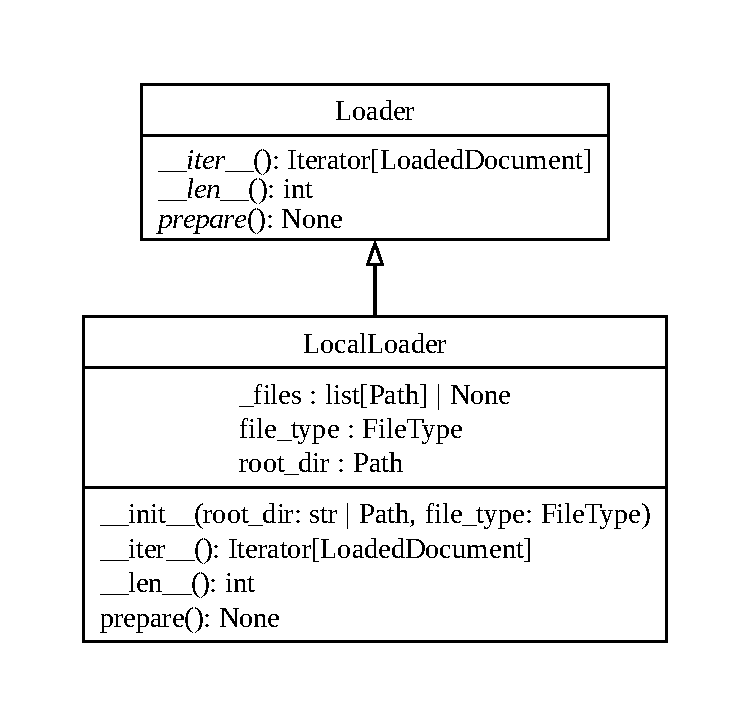
\includegraphics[width=\textwidth, height=0.7\textwidth, keepaspectratio]{res/classes/cls_loaders.pdf}
    \caption{Diagram tříd pro načítání dokumentů z~disku}
    \label{fig:loaders}
\end{figure}



\subsection{Zpracování}
Třída \verb"DocumentIngestor" se s~předanou instancí \verb"LocalLoader" postará o~postupné zpracování každého načteného \verb"PDF" dokumentu pomocí knihovny \product{pdfplumber} \cite{pdfplumber}. Ta dokáže binární data dokumentu zpracovat na text (bez obrázků) a uložit ho do databázové tabulky \verb"DOCUMENT" s~potřebnými metadaty.

Třída \verb"GoldenDatasetIngestor" načítá soubory typu \verb"JSON", které reprezentují zlatý dataset. Jeden dokument má jeden zlatý dataset. Všechny tyto soubory jsou definovány konstantou \verb"GOLDEN_PATH" v~souboru \verb"textractor.py", standardně se nachází ve složce \filename"data/golden_seed/". Diagram tříd pro zpracování vstupních dokumentů je zobrazen na obrázku \ref{fig:ingestors}.

\begin{figure}[]
    \centering
    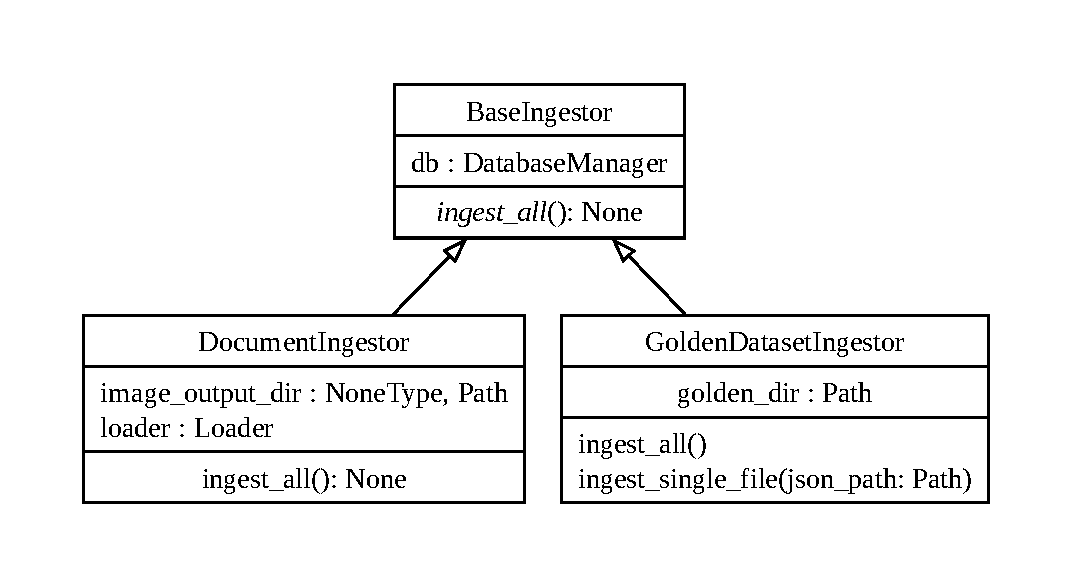
\includegraphics[width=\textwidth]{res/classes/cls_ingestors.pdf}
    \caption{Diagram tříd sloužící pro uložení dokumentů do databáze}
    \label{fig:ingestors}
\end{figure}

\subsubsection{Ukládání obrázků}
Dokument může obsahovat obrázky. Je možné předat třídě \verb"DocumentIngestor" parametr \verb"image_output_dir" s~cestou ke složce, do které se mají ukládat obrázky z~dokumentu. O~extrakci obrázků z~dokumentů se stará knihovna \product{pypdfium2} \cite{pypdfium}. Ta z~bajtů dokumentu nalezne obrázky, které jsou následně uloženy v~podsložce s~názvem daného dokumentu.

\subsubsection{Struktura zlatého datasetu}
Zlatý dataset má pevně danou strukturu, která je kontrolována knihovnou \product{pydantic}. Definice tohoto \product{pydantic} schématu je zobrazena ve výpisu \ref{lst:pydantic-golden-dataset-schema}.

\nopagebreak 
\begin{code}{python}{Definice pydantic schématu zlatého datasetu\label{lst:pydantic-golden-dataset-schema}}
class GoldenDatasetSchema(BaseModel, Generic[T]):
    """Generic wrapper for the golden dataset schema."""
    document_filename: str
    golden_parameters: List[GoldenParameter[T]]
\end{code}

Každý soubor ze zlatého datasetu obsahuje název dokumentu, ze kterého byly požadavky extrahovány, a seznam \term{zlatých parametrů}, které jsou reprezentovány strukturou \verb"GoldenParameter". Zlatý parametr je reprezentován dalším vnořeným \product{pydantic} schématem, které obsahuje \textbf{strukturu informací, ve které chce uživatel dostávat výstupy od jazykového modelu}. Jedná se o~formalizovaný parametr z~konkrétního požadavku z~extrakční fáze. Schéma zlatého parametru je znázorněno ve výpisu \ref{lst:pydantic-golden-parameter}.

\nobreakstart
        \begin{code}{python}{Definice pydantic schématu zlatého parametru\label{lst:pydantic-golden-parameter}}
            class GoldenParameter(BaseModel, Generic[T]):
            """Represents a single analyzed parameter."""
            raw_text: str = Field(..., description="Extracted text from the document (Phase 1).")
            analyzed_data: T = Field(..., description="Analyzed text from the document (Phase 2). This is the 'golden' expected output for the LLM to match.")
        \end{code}
\nobreakend

Zástupný symbol \verb"T" reprezentuje schéma pro strukturu formalizovaných dat, \textbf{které si uživatel může přizpůsobit podle povahy vstupních dokumentů a požadavků, které chce extrahovat}. Pro specifikace požadavků na software byly tedy vybrány hledané atributy:
\begin{itemize}
    \item \verb"raw_text": zkopírovaný text, který byl extrahován z~dokumentu v~extrakční fázi (fáze 1),
    \item \verb"analyzed_data": obsahuje atribut \verb"parsed_requirements" (fáze 2), což je seznam formalizovaných parametrů požadavku z~atributu \verb"raw_text"; každý požadavek obsahuje atribut \verb"requirement_summary", což je stručný popis požadavku, a volitelný atribut \verb"parameters" reprezentující \textbf{seznam kvantifikovatelných dat}, která byla z~požadavku vyextrahována.
\end{itemize}
Počítá se s~tím, že každý záznam z~tabulky \verb"EXTRACTED_TEXT" musí obsahovat jeden požadavek a tento požadavek musí obsahovat jeden formalizovaný požadavek -- tedy jeden záznam v~tabulce \verb"ANALYZED_TEXT". \textbf{Jeden extrahovaný požadavek může formalizovat více modelů.}

Příklad zlatého datasetu se dvěma extrahovanými požadavky pro konkrétní dokument je zobrazen ve výpisu \ref{lst:json-golden-dataset}. Jde o~dokument s~názvem \filename"SRS_WebGLGame.pdf" (Hra), který obsahuje specifikace požadavků na software pro návrh hry využívající \verb"WebGL" (více popsáno v~kapitole \ref{sec:vyhodnoceni}). Každý záznam v~seznamu \verb"golden_parameters" reprezentuje jeden zkopírovaný text z~dokumentu (fáze 1), který obsahuje požadavek a jeho formalizaci do strukturovaných dat (fáze 2).

\nobreakstart
\lstset{style=json}
\begin{lstlisting}[caption=Příklad zlatého požadavku ve formátu \texttt{JSON}, label=lst:json-golden-dataset]
{
    "document_filename": "SRS_WebGLGame.pdf",
    "golden_parameters": [
                {
            "raw_text": "Client should be able to render the scene at at least 30 FPS",
            "analyzed_data": {
                "parsed_requirements": [
                    {
                        "requirement_summary": "client should render the scene at min 30 FPS",
                        "parameters": [
                            {
                                "parameter_value": 30,
                                "parameter_unit": "FPS"
                            }
                        ]
                    }
                ]
            }
        }
    ]
}
\end{lstlisting}
\nobreakend

\section{Dvě fáze zpracování jazykovým modelem}
%Program pracuje ve dvouch hlavních fázích zpracování jazykovým modelem -- \textbf{Extrakční fáze (Fáze 1)} a \textbf{Formalizační fáze (Fáze 2)}. Obě fáze jsou na sobě nezávislé a dají se spouštět odděleně, avšak formalizační fáze závisí na výstupu extrakční fáze. Je tedy nutné, aby databáze obsahovala extrahované texty, jinak LLM nemá z čeho analyzovat data.

Ve složce \filename"src/pipeline/" se nachází soubory, které implementují dvě fáze zpracování dokumentů jazykovým modelem -- \textbf{extrakční fáze (fáze 1)} a \textbf{formalizační fáze (fáze 2)}. Každá z~těchto fází je implementována jako samostatná třída, která se stará o~správné posílání textů z~dokumentů do jazykového modelu. Diagram těchto tříd je zobrazen na obrázku \ref{fig:pipeline}.

\begin{figure}[]
    \centering
    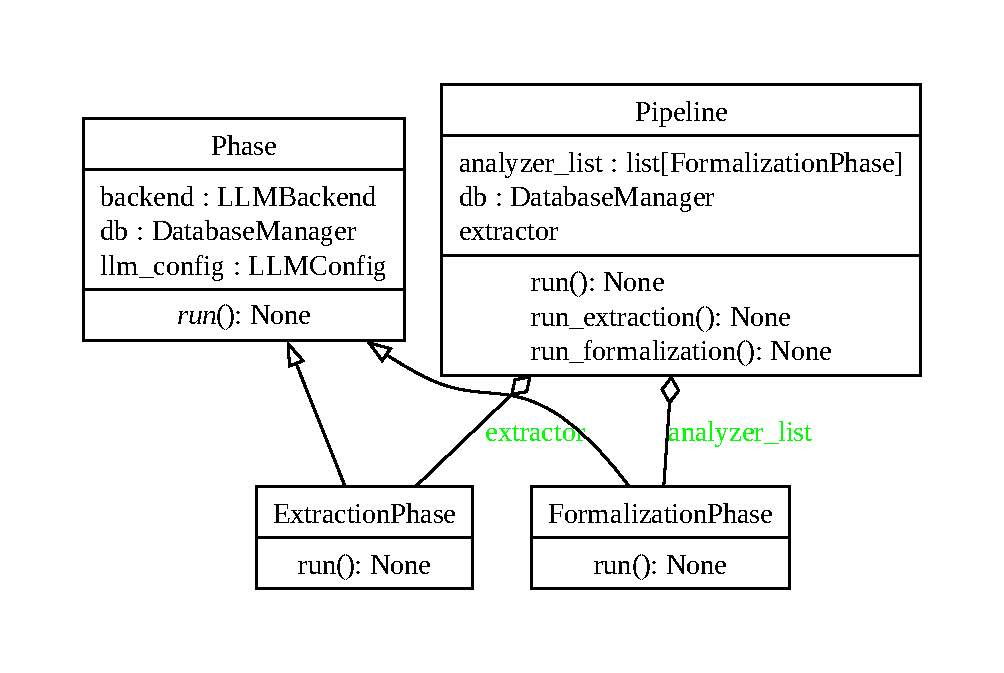
\includegraphics[width=\textwidth]{res/classes/cls_pipeline.pdf}
    \caption{Diagram tříd pro fáze zpracování dokumentů jazykovým modelem}
    \label{fig:pipeline}
\end{figure}

Třída \verb"Phase" je předek (a abstraktní třída) pro obě fáze zpracování -- třídy \\ \verb"ExtractionPhase" a \verb"FormalizationPhase". Obsahuje společné metody a atributy, které jsou sdílené mezi oběma fázemi, jako například metoda \verb"process_document", která zajišťuje načítání textu z~dokumentu a posílání ho do jazykového modelu.


Ve třídě \verb"Pipeline" je implementována logika pro spouštění obou fází zpracování. Tato třída umožňuje spustit pouze extrakční fázi, pouze formalizační fázi, nebo obě fáze postupně. Tímto způsobem lze flexibilně řídit celý proces zpracování dokumentů jazykovým modelem.

\section{Jazykové modely}
Pro komunikaci s~jazykovými modely je ve složce \filename"src/llms/" vytvořen soubor \verb"backends.py", jehož obsah zajišťuje volání velkých jazykových modelů přes jejich \verb"API". Podporované \verb"API" jazykových modelů jsou:
\begin{itemize}
    \item od společnosti OpenAI: \verb"gpt-5.4-nano" \cite{llm-gptnano},
    \item od společnosti Mistral: \verb"mistral-large-latest" \cite{llm-mistral}
    \item od společnosti Meta: \verb"llama3.2:latest" \cite{llm-llama}.
\end{itemize}

Třídy na diagramu \ref{fig:backends} tedy reprezentují jednotlivé obaly pro komunikaci s~těmito API jazykových modelů.

\begin{figure}[]
    \centering
    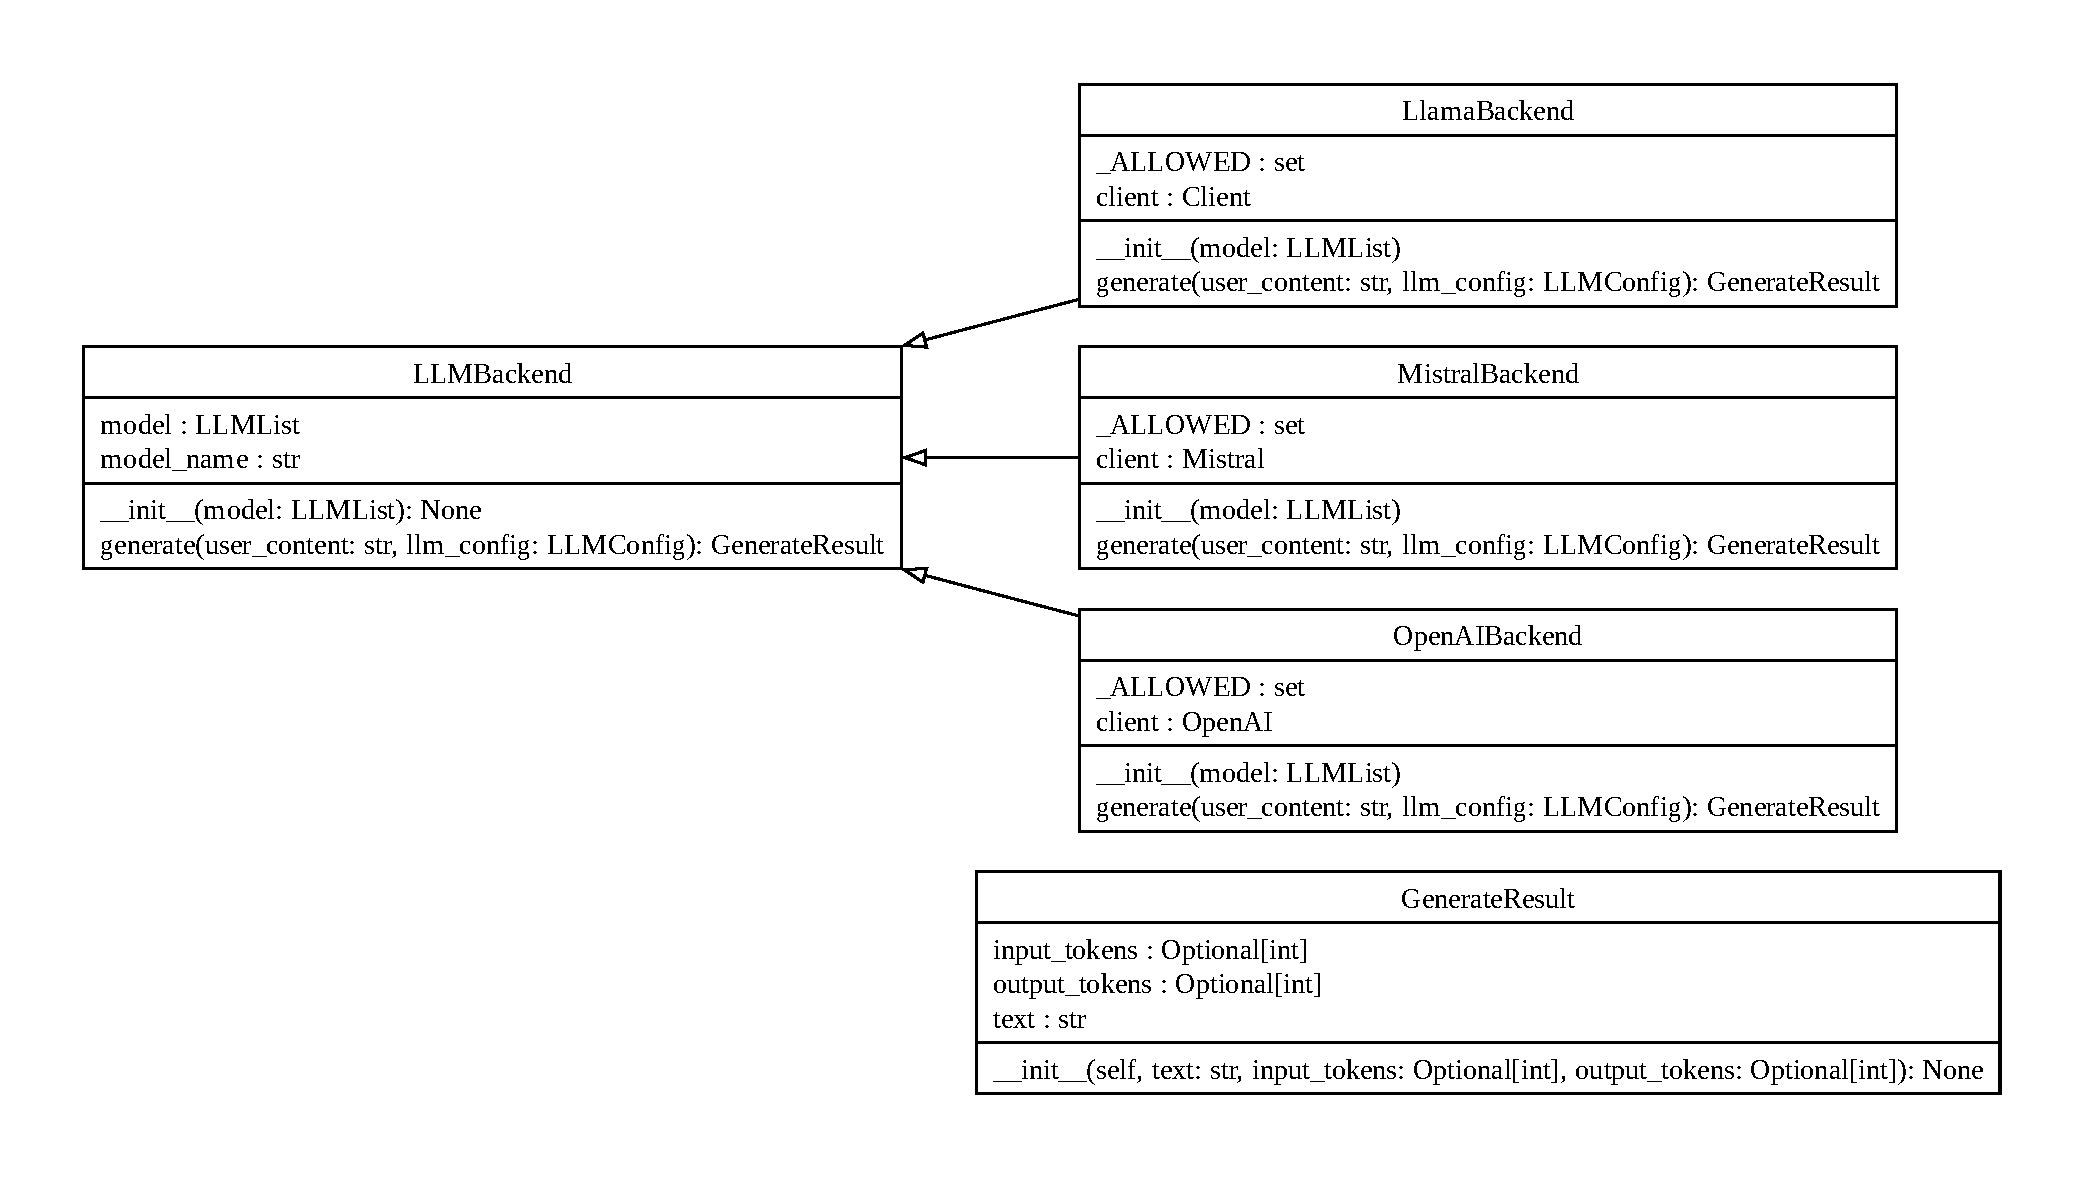
\includegraphics[width=\textwidth]{res/classes/cls_backends.pdf}
    \caption{Diagram tříd sloužících pro komunikaci s~jazykovými modely}
    \label{fig:backends}
\end{figure}

Pro přidání jazykového modelu k~existujícím třídám stačí přidat název modelu do výčtové třídy \verb"LLMList" v~souboru \filename"src/llms/config.py" a klíč výčtu s~tímto názvem modelu přidat do množiny povolených modelů (konstant \verb"_ALLOWED") k~příslušnému potomkovi třídy \verb"LLMBackend".

Pro přidání nového jazykového modelu, který není od výše zmíněných společností, je nutné přidat nového potomka třídy \verb"LLMBackend" a nastavit \verb"API" pro komunikaci s~tímto modelem.

\subsection{Konfigurace jazykového modelu}
Každý jazykový model má své specifické parametry, které se nastavují v~souboru \filename"src/llms/config.py" v~datové třídě \verb"LLMConfig". Instanci této třídy přebírá metoda \verb"generate" v~potomkovi třídy \verb"LLMBackend". Tato konfigurace obsahuje parametry:
\begin{itemize}
    \item \verb"system_content": Systémová zpráva, která obsahuje instrukce pro jazykový model, jak má zpracovat zadaný text. Tato zpráva je důležitá pro správné fungování extrakční a formalizační fáze, protože určuje, jaké informace má jazykový model hledat a jak má strukturovat svůj výstup. Systémová zpráva pro extrakční fázi (fázi 1) je uvedena v~příloze \ref{pril:system-message-extraction} a pro formalizační fázi (fázi 2) v~příloze \ref{pril:system-message-formalization}.
    \item \verb"response_schema": Schéma (\product{pydantic}), které definuje strukturu výstupu z~jazykového modelu. Schémata jsou dále popsána v~sekci \ref{sec:llm-schemas}.
    \item \verb"name": Označení dané instance konfigurace LLM.
\end{itemize}

Systémové zprávy jsou uloženy v~souboru \filename"src/llms/config.py" a \textbf{je vhodné je změnit a přizpůsobit pro konkrétní typ dokumentů a informací, které se pomocí LLM extrahují a formalizují}.

\subsection{Schémata pro jazykové modely}\label{sec:llm-schemas}
Výstupy z~jazykových modelů musí být striktně typovány na příslušná \textbf{schémata} definována v~souboru \filename"src/llms/schemas.py". Tato schémata jsou definována pomocí knihovny \product{pydantic}, která zajišťuje, že jazykový model vrátí data přesně v~této struktuře. Všechny API použitých jazykových modelů umožňují využít toto ověření.

Schéma pro \textbf{extrakční fázi} je definováno třídou \verb"ExtractionOutputSchema", která obsahuje atribut \verb"raw_text", což je seznam zkopírovaných textů z~dokumentu, které jazykový model identifikoval jako požadavky. Schéma je zobrazeno ve výpisu \ref{lst:extracted-text-schema}. \textbf{Toto schéma není vhodné měnit, protože je pevně dané pro extrakční fázi a jazykový model musí vracet výstup přesně v~tomto formátu.}

\nobreakstart
\begin{code}{python}{Definice schématu pro extrakční fázi\label{lst:extracted-text-schema}}
class ExtractedTextSchema(BaseModel):
"""Output schema for Phase 1 -- extraction."""
raw_text: list[str]
\end{code}
\nobreakend

Pro \textbf{formalizační fázi} je definováno schéma \verb"AnalyzedTextSchema", které obsahuje atribut \verb"parsed_requirements", což je seznam formalizovaných požadavků, které jazykový model identifikoval z~extrahovaných textů z~fáze 1. Každý formalizovaný požadavek obsahuje atribut \verb"requirement_summary", což je stručný popis požadavku, a volitelný atribut \verb"parameters", který reprezentuje seznam kvantifikovatelných dat, která byla z~požadavku vyextrahována. Tato schémata pro formalizační fázi jsou zobrazena ve výpisu \ref{lst:analyzed-text-schema}. \textbf{V~těchto schématech je vhodné upravit strukturu formalizovaných dat podle povahy vstupních dokumentů a dat, které je potřeba extrahovat. Není přitom potřeba měnit proces ukládání do databáze.}

\nobreakstart
\begin{code}{python}{Definice schématu pro formalizační fázi\label{lst:analyzed-text-schema}}
class QuantifiableData(BaseModel):
    """A single quantifiable parameter extracted from a requirement."""
    parameter_value: float | None
    parameter_unit: str | None


class ParsedRequirement(BaseModel):
    """Single requirement parsed into a structured form."""
    requirement_summary: str
    parameters: list[QuantifiableData] = []


class AnalyzedTextSchema(BaseModel):
    """Output schema for Phase 2 -- formalization."""
    parsed_requirements: list[ParsedRequirement]
\end{code}
\nobreakend

\section{Vyhodnocovací prostředí Textractor Studio}
Pro potřeby vyhodnocení výsledků výstupů z~jazykových modelů bylo potřeba vytvořit grafické uživatelské rozhraní \term{Textractor Studio}. Pro jeho tvorbu byla zvolena knihovna \product{streamlit} \cite{streamlit}, která umožňuje vytvářet interaktivní webové aplikace v~jazyce \product{Python}. Soubory se třídami tvořícími toto grafické uživatelské rozhraní se nacházejí ve složce \filename"src/gui/" a diagram těchto tříd je zobrazen na obrázku \ref{fig:cls_gui} v~příloze \ref{pril:cls_gui}.

Každý režim vyhodnocení má svoji vlastní třídu, která se stará o~přebírání dat z~databáze a jejich zobrazení v~uživatelském rozhraní. Třída \verb"BaseEvaluator" zajišťuje společné funkce pro obě fáze vyhodnocení, jako například přebírání společných záznamů z~databáze. Třídy \verb"ProductionEvaluator" a \verb"BenchmarkEvaluator" implementují vlastní metody pro každý režim vyhodnocení. Jelikož knihovna \product{streamlit} spouští celý kód znovu při každé interakci uživatele, \textbf{režim nejde změnit při běhu aplikace}, ale je potřeba znovu spustit Textractor Studio s~nastaveným režimem, který se určuje podle proměnné prostředí (v~souboru \filename".env") pomocí proměnné \verb"MODE", která může nabývat hodnoty \uv{production} pro produkční režim nebo \uv{benchmark} pro evaluační režim. Bez zadání tohoto parametru se spustí evaluační režim.

\subsection{Rozložení GUI}
Uživatelské rozhraní je rozděleno na boční panel (vlevo) a hlavní obsah (vpravo). Náčrt rozložení grafického uživatelského rozhraní je zobrazen na obrázku \ref{fig:wireframe}.

\begin{figure}
    \centering
    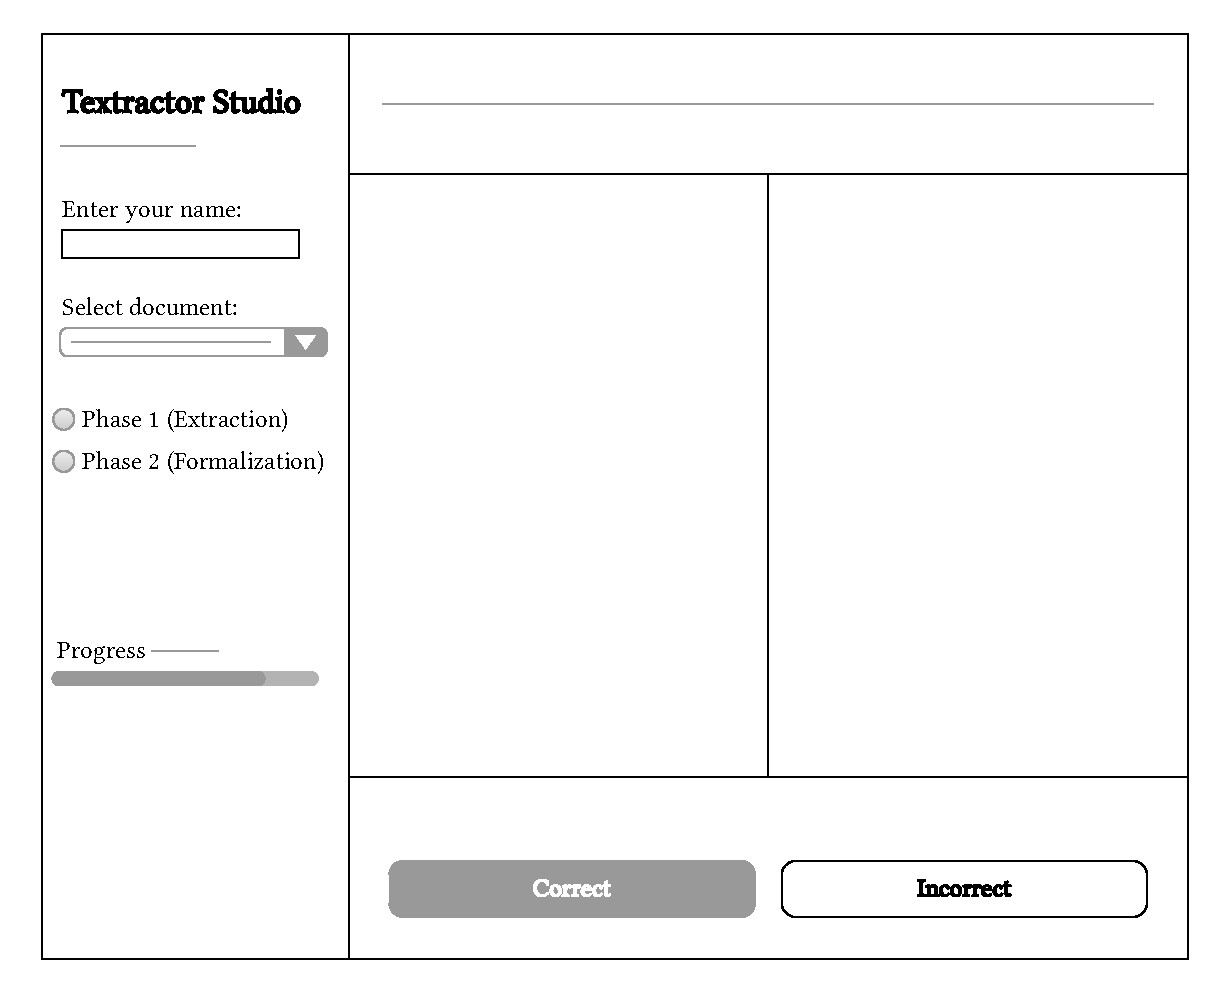
\includegraphics[width=\textwidth]{res/wireframe.pdf}
    \caption{Náčrt rozložení grafického uživatelského rozhraní Textractor Studio}
    \label{fig:wireframe}
\end{figure}

\subsubsection{Boční panel}
V~bočním panelu je pro přehlednost hodnotitelů \textbf{nutné} zadat jméno (tomu odpovídá atribut \verb"evaluator_name" v~databázových tabulkách \verb"EXTRACTED_TEXT_EVAL" a \verb"ANALYZED_TEXT_EVAL"). Dále je nutné vybrat, \textbf{který dokument se bude hodnotit}. V~produkčním režimu se zobrazují všechny dokumenty, zatímco v~evaluačním režimu se zobrazují pouze dokumenty, pro které existuje zlatý dataset.

Přepínačem ve spodní části bočního panelu je nutné zvolit, kterou fázi bude uživatel vyhodnocovat, tedy extrakční nebo formalizační.

\subsubsection{Hlavní obsah}
V~hlavním obsahu se zobrazuje seznam záznamů z~databáze, které \textbf{odpovídají zvolenému dokumentu a fázi}. Oba režimy mají různé rozložení pro obě fáze, jelikož výstupem obou režimů je jiný typ vyhodnocení. 

V~\textbf{produkčním režimu fáze 1} se zobrazuje zkopírovaný text, který jazykový model identifikoval jako požadavek, a vedle něj se nachází náhled dokumentu, ze kterého byla data extrahována (pomocí knihovny \product{streamlit\_pdf\_viewer} \cite{streamlit-pdf}). Uživatel musí zkontrolovat, zda se tento zkopírovaný text skutečně v~dokumentu nachází a označit ho jako správný nebo nesprávný.

V~\textbf{produkčním režimu fáze 2} se zobrazuje postupně každý zkopírovaný text, který byl označen jako správný v~extrakční fázi (tedy se v~dokumentu skutečně nachází). Vedle něj se zobrazuje jeho formalizace, u~které musí uživatel zkontrolovat správnost a označit ji jako správnou nebo nesprávnou.

V~\textbf{evaluačním režimu fáze 1} se zobrazuje každý zkopírovaný text, který jazykový model identifikoval jako požadavek, a vedle něj se zobrazuje seznam zlatých požadavků z~ručně vytvořeného zlatého datasetu. Hodnotitel musí vybrat a \uv{propojit} zkopírovaný text s~některým ze zlatých požadavků (pomocí atributu \verb"matched_golden_id") a označit, že se shodují. Pokud hodnotitel zjistí, že se ve zlatém datasetu tento požadavek nevyskytuje, označí ho jako nesprávný.

\textbf{Evaluační režim fáze 2} zobrazuje \textbf{ve formě karet}\footnote{Struktura karty odpovídá struktuře třídy \verb"ParsedRequirement" ze schématu ve výpisu \ref{lst:analyzed-text-schema}.} každý formalizovaný požadavek z~jazykového modelu (vlevo) a vedle něj (vpravo) zobrazuje formalizovaný požadavek ze zlatého datasetu. Uživatel musí porovnat oba formalizované požadavky a označit, zda se shodují, nebo ne. Může se stát, že jazykový model požadavek formalizoval \uv{do více karet}\footnote{Stále se jedná o~formalizaci jednoho požadavku.}, proto je potřeba porovnat všechny karty. V~takovém případě je možné karty ručně spárovat -- to je umožněno jejich vizuálním označením. Toto označení je zobrazeno pouze na úrovni uživatelského rozhraní a nemá žádný vliv na data uložená v~databázi.


\section{Logování}

Aplikace využívá standardní knihovnu \texttt{logging} jazyka \product{Python}, obalenou do pomocné třídy \texttt{Log} (v~souboru \filename"src/utils.py") a doplněnou o~mechanismus potlačení výstupu do konzole při zobrazení průběhového ukazatele (knihovnou \product{tqdm} \cite{tqdm}).

Třída \texttt{Log} obsahuje čtyři statické metody odpovídající úrovním závažnosti:

\begin{itemize}
    \item \texttt{debug(message: str, source=None)} -- podrobné diagnostické informace, které se zapisují jen do souboru,
    \item \texttt{info(message: str, source=None)} -- běžné provozní zprávy (zahájení extrakce nebo formalizace, výsledky operací),
    \item \texttt{warning(message: str, source=None)} -- neočekávané, ale zvládnutelné situace,
    \item \texttt{error(message: str, source=None)} -- chyby, po nichž zpracování daného záznamu přeskočí.
\end{itemize}

Každá tato metoda předá zprávu metodě \verb"_log(level, message, source)" třídy \verb"Log" (ta volá standardní \verb"logging" systém), která z~parametru \texttt{source} odvodí název komponenty, ze které log pochází. Pokud je \texttt{source} instancí třídy, použije se její název (například \texttt{ExtractionPhase}), jinak se použije řetězec \uv{root}. Tím je každá zpráva v~logu automaticky přiřazena ke komponentě, která ji vyvolala.


\subsection{Inicializace}
Metoda \verb"setup_logging(log_to_file: bool = True)" třídy \verb"Log" se volá jednou při startu aplikace a konfiguruje globální logovací systém prostřednictvím metody \texttt{logging.basicConfig()}.

Hlavní logger je nastaven na úroveň \texttt{DEBUG}, aby vypisoval veškeré zprávy. Filtrování probíhá až na úrovni handlerů:

\begin{itemize}
    \item \textbf{StreamHandler (konzole)} -- zobrazuje zprávy úrovně \texttt{INFO} a výše. Ladící zprávy (\texttt{DEBUG}) se do konzole nevypisují.
    \item \textbf{FileHandler (soubor)} -- zapisuje zprávy úrovně \texttt{DEBUG} a výše. Soubor nese název ve formátu \verb"DD_MM_YYYY_HH_MM_SS.log" a ukládá se do adresáře \filename"logs/".
\end{itemize}

Formát každé zprávy je jednotný:

\lstset{style=plain}
\begin{lstlisting}
[HH:MM:SS:mmm][ÚROVEŇ][Komponenta] Text zprávy
\end{lstlisting}

Příklad záznamu logu o~extrakci dokumentu může vypadat například takto:
\lstset{style=plain}
\begin{lstlisting}
[14:33:51:277][INFO][ExtractionPhase] Extracting 'thesis.pdf' (doc_id=3)...
\end{lstlisting}

\subsection{Průběhový ukazatel}

Průběhový ukazatel knihovny \texttt{tqdm} a souběžný výpis logů do konzole by se navzájem rušily -- každý řádek logu by rozbil vykreslení ukazatele. Proto je při každém zobrazení průběhového ukazatele konzolový výstup dočasně potlačen. % pomocí kontextového manažeru \verb"_suppress\_console\_handlers()}.

%\subsection{Přehled úrovní a cílů výstupu}
Tabulka \ref{tab:log-levels} shrnuje, které úrovně zpráv se zobrazují v~konzoli a které se zapisují do logovacího souboru. Zprávy úrovně \texttt{DEBUG} jsou určeny pro podrobné sledování průběhu a diagnostiku, ale nejsou zobrazeny v~konzoli, aby nerušily uživatele. Zprávy úrovně \texttt{INFO} a výše jsou zobrazeny v~konzoli i zapsány do souboru, protože obsahují klíčové informace o~průběhu zpracování a případných problémech.

\begin{table}[]
\centering
\caption{Výstupy zpráv jednotlivých úrovní}
\label{tab:log-levels}
\begin{tabular}{lcc}
\hline\hline
\textbf{Úroveň} & \textbf{Konzole} & \textbf{Soubor} \\
\hline
\texttt{DEBUG}   & ne  & ano \\
\texttt{INFO}    & ano & ano \\
\texttt{WARNING} & ano & ano \\
\texttt{ERROR}   & ano & ano \\
\hline\hline
\end{tabular}
\end{table}

% =================================================================================
% Otestujte navržené řešení s několika vybranými LLM a posuďte jejich stávající schopnost úlohu řešit
% =================================================================================
\chapter{Vyhodnocení a testování}\label{sec:vyhodnoceni}
V~této kapitole je popsána analýza výsledků z~extrakční a formalizační fáze, které byly vytvořeny rozhraním Textractor Studio. Obsahuje různé metriky, které byly vypočteny pro otestování schopnosti různých velkých jazykových modelů extrahovat data z~dlouhých textů. \textbf{Prezentované výsledky jsou výsledkem analýzy výstupů pouze evaluační fáze rozhraní Textractor Studio.}

\section{Datový korpus}\label{sec:korpus}
Pro potřeby tohoto vyhodnocení byly ručně analyzovány dva dokumenty typu \verb"PDF" -- specifikace softwarových požadavků:
\begin{enumerate}
    \item \textbf{WebGL Card Game Platform}: Specifikace požadavků na platformu karetních her založenou na webovém rozhraní, vytvořenou pomocí technologie WebGL \cite{doc-hra}. Tento dokument je označován jako \term{Hra}.
    \item \textbf{Nemocniční informační systém}: Technická specifikace dodávky nového nemocničního informačního systému pro Vojenskou nemocnici Brno \cite{doc-nis}. Tento dokument je označován jako \term{NIS}. 
\end{enumerate}

\subsection{Parametry testovacích dokumentů}
Při výběru testovacích dat byl kladen důraz na to, aby jeden dokument byl delší a jeden kratší. Zároveň je důležité testovaní na dokumentech psaných v~českém i anglickém jazyce, protože jazykové modely byly vyzvány k~přizpůsobení se danému jazyku. Potřebné parametry těchto dokumentů jsou zobrazeny v~tabulce \ref{tab:parametry-golden-doc}.

\begin{table}[h! ]
\centering
\caption{Parametry testovacích dokumentů}
\label{tab:parametry-golden-doc}
\begin{tabularx}{\textwidth}{lXX}
\hline\hline
 & \textbf{Hra} & \textbf{NIS} \\ \hline
Jazyk                                        & Anglický & Český \\
Počet stran                                  & 28       & 106   \\
Počet ručně identifikovaných požadavků       & 107      & 984   \\
\hline\hline
\end{tabularx}
\end{table}


Pro oba testovací dokumenty proběhla ruční analýza všech požadavků a byl pro ně vytvořen zlatý dataset.

\section{Testovací parametry}
V~této sekci jsou popsány vybrané modely a počítání cen extrakce a formalizace. Systémová zpráva, která definuje roli pro jazykový model a příkazy pro extrakci je obsažena v~příloze \ref{pril:system-message-extraction}. Pro formalizaci je zpráva vypsána v~příloze \ref{pril:system-message-formalization}.

\subsection{Vybrané modely}\label{sec:vybrane-modely}
Jelikož Textractor funguje ve dvou fázích, pro extrakci i formalizaci požadavků \textbf{je možné zvolit jiný model}. Tabulka \ref{tab:pouzite-llms} ukazuje použité modely v~obou těchto fázích.

Byly použité modely od společnosti OpenAI, konkrétně \verb"gpt-5.4-nano" \cite{llm-gptnano} a od společnosti Mistral (model \verb"mistral-large-latest" \cite{llm-mistral} -- konkrétně Mistral 3 Large). Pro kratší dokument byl také vyzkoušen ve formalizační fázi lokální model \verb"llama3.2:latest" \cite{llm-llama} od společnosti Meta. Tento model nebyl spouštěn v~extrakční fázi ani pro delší dokument NIS z~důvodu časové náročnosti běhu. Model \verb"mistral-large-latest" nebyl schopen vyextrahovat dokument NIS. V~odpovědi API požadavku na extrakci tohoto dokumentu se nacházela i po opakování pokusu chyba HTTP 503 a zpráva \uv{Internal server error} s~hodnotou parametru \verb"type" \uv{unreachable\_backend}.

Při prvních testech programu Textractor byl vyzkoušen také model \verb"gpt-4o" \cite{llm-gpt4o} od společnosti OpenAI, který je vhodný pro analýzu dlouhých textů \cite{openai-platform-models}. Jenže díky jeho maximálnímu počtu výstupních tokenů (16 384) nebylo možné v~extrakční fázi zpracovat \textbf{celý} dokument NIS -- model vrátil jen část do obsažení limitu, proto tento model nebyl do hodnocení zahrnut.

\begin{table}[h!]
\catcode`-=12
\centering
\caption{Použité jazykové modely pro vyhodnocení pro dokumenty podle fází}
\label{tab:pouzite-llms}
\begin{tabularx}{\textwidth}{l|XX}
\hline
\multicolumn{1}{c|}{\multirow{2}{*}{\textbf{Dokument}}} & \multicolumn{2}{c}{\textbf{Modely}}                                                                                                   \\ \cline{2-3} 
\multicolumn{1}{c|}{}                                   & \textbf{Fáze 1}                                      & \textbf{Fáze 2}                                                                \\ \hline\hline
Hra                                                     & \texttt{gpt-5.4-nano}, \texttt{mistral-large-latest} & \texttt{gpt-5.4-nano}, \texttt{mistral-large-latest}, \texttt{llama3.2:latest} \\
NIS                                                     & \texttt{gpt-5.4-nano} & \texttt{gpt-5.4-nano},  \texttt{mistral-large-latest}\\
\hline\hline
\end{tabularx}
\end{table}

\subsection{Ceny}
Ve vyhodnocení se objevuje porovnání cen a extrakcí. Společnosti účtují využití jazykových modelů přes API pomocí dvou ukazatelů -- vstupních tokenů a výstupních tokenů. Tyto ceny se uvádí za 1 milion tokenů v~amerických dolarech. Tabulka \ref{tab:ceny-za-api} ukazuje ceny pro použité modely podle ceníků na  webových stránkách společností (pro OpenAI \cite{gpt-api-pricing}, pro Mistral \cite{mistral-api-pricing}) k~datu spuštění extrakce a formalizace, tedy 3. 4. 2026.

\begin{table}[h!]
\centering
\caption{Ceny vstupních a výstupních tokenů pro LLM}
\label{tab:ceny-za-api}
\begin{tabular}{lcc}
\hline\hline
\textbf{Model} & \textbf{Vstupní tokeny} & \textbf{Výstupní tokeny} \\
\hline
\texttt{gpt-5.4-nano}   & 0,2 \$ / 1M tokenů & 1,25 \$ / 1 M tokenů \\
\texttt{mistral-large-latest}   & 0,5 \$ / 1 M tokenů & 1,5 \$ / 1 M tokenů \\
\hline\hline
\end{tabular}
\end{table}

Model \verb"llama3.2:latest" v~tabulce chybí, jelikož byl spuštěn lokálně na osobním notebooku\footnote{Notebook s~procesorem Intel Core i5 1335U Raptor Lake a integrovanou grafickou kartou Intel Iris Xe Graphics.}. Cena vstupních a výstupních tokenů u~tohoto modelu je počítána jako 0 Kč.

Pro lepší přehlednost byly ceny převedeny na české koruny podle kurzu 20,608 Kč za 1 \$ (k~datu 17. 4. 2026) \cite{kurz}.

\section{Časy}\label{sec:vyhodnoceni-srovnani-casu}
V~tabulce \ref{tab:prumerne-casy-extrakce} jsou vypsány \textbf{průměrné ceny a časy extrakce jednoho dokumentu podle modelů}\footnote{Jak bylo zmíněno v~sekci \ref{sec:vybrane-modely}, model \verb"mistral-large-latest" nebyl schopen zpracovat dokument NIS.}. Modelu \verb"mistral-large-latest" trvalo několikanásobně větší čas extrahovat požadavky z~kratšího dokumentu Hra, a to i s~vyšší cenou.

\begin{table}[h!]
\centering
\caption{Průměrné ceny a časy extrakce za dokument podle modelů}
\label{tab:prumerne-casy-extrakce}
\begin{tabularx}{\textwidth}{llXX}
\hline\hline
\textbf{Dokument} & \textbf{Model} & \textbf{Průměrný čas extrakce} & \textbf{Průměrná cena extrakce} \\
\hline
NIS & \texttt{gpt-5.4-nano}     & 222,61 s~& 1,30 Kč \\
\midrule
\multirow{2}{*}{Hra}             & \texttt{gpt-5.4-nano}     &  18,62 s~& 0,11 Kč \\
                                & \texttt{mistral-large-latest} &  75,37 s~& 0,19 Kč\\
\hline\hline
\end{tabularx}
\end{table}

V~tabulce \ref{tab:prumerne-casy-formalizace} jsou vypsány \textbf{průměrné ceny a časy formalizace jednoho požadavku podle modelů}. Ve formalizační fázi model \verb"gpt-5.4-nano" také dominuje v~průměrné rychlosti formalizace na jeden požadavek. V~dokumentu Hra je však o~0,14 s~rychlejší než u~dokumentu NIS, což je způsobeno tím, že v~tomto dokumentu byly celkově extrahovány kratší věty. Časově nejhorší je však model \verb"llama3.2:latest", kterému trvalo průměrně jeden požadavek v~dokumentu Hra extrahovat za 9,74 sekundy.

\begin{table}[h!]
\centering
\caption{Průměrné ceny a časy formalizace za požadavek podle modelů}
\label{tab:prumerne-casy-formalizace}
\begin{tabularx}{\textwidth}{llXX}
\hline\hline
\textbf{Dokument} & \textbf{Model} & \textbf{Průměrný čas} & \textbf{Průměrná cena} \\
\midrule
\multirow{2}{*}{NIS}
    & \texttt{gpt-5.4-nano}         & 1,49 s~& 0,0057 Kč \\
    & \texttt{mistral-large-latest} & 5,43 s~& 0,0379 Kč \\
\midrule
\multirow{3}{*}{Hra}
    & \texttt{gpt-5.4-nano}         & 1,35 s~& 0,0047 Kč \\
    & \texttt{llama3.2:latest}      & 9,74 s~& 0 Kč \\
    & \texttt{mistral-large-latest} & 4,26 s~& 0,0308 Kč \\
\hline\hline
\end{tabularx}
\end{table}

\textbf{Celkový čas ruční extrakce a formalizace těchto dokumentů (tedy tvorba zlatého datasetu) trval pro dokument Hra přibližně 2 hodiny a pro dokument NIS přibližně 14 hodin a 30 minut.}

\section{Kvalita}\label{sec:vyhodnoceni-kvalita}
Kvalita modelů byla také měřena podle fází. V~extrakční fázi byl pro každý LLM vypočítán recall (vzorec \ref{eq:recall}), což označuje, \textbf{kolik procent ze všech reálně existujících požadavků (to, co našel člověk ve zlatém datasetu) model dokázal najít}. Dále byla použita metrika precision (vzorec \ref{eq:precision}), která ukazuje, \textbf{kolik procent z~toho, co model celkem vyprodukoval, bylo skutečně správně}. Posledním ukazatelem je F1 skóre (vzorec \ref{eq:f1}), které spojí tyto metriky dohromady a vytvoří celkové hodnocení výkonu harmonickým průměrem hodnot recall a precision.

Ve formalizační fázi byla spočítána metrika accuracy (sekce \ref{sec:mereni-uspesnosti}, vzorec \ref{eq:acc}), která označuje, kolik procent \textbf{z~hodnocených formalizací} model zvládl vygenerovat správně (to jsou formalizace, ve kterých nic nechybělo a nic chybného nepřebývalo). Formalizace vyprodukované modelem byly prováděny jen nad zlatými záznamy z~extrakční fáze (fáze 1). 

\subsection{Extrakce}
V~extrakční fázi byly v~rozhraní Textractor Studio ohodnoceny všechny provedené extrakce všemi použitými modely pro dané dokumenty. Tabulka \ref{tab:extrakce-vysledky} ukazuje F1 skóre, precision a recall podle modelů pro oba dokumenty v~extrakční fázi. Jsou v~ní zobrazeny také hodnoty, podle kterých se tyto metriky vypočetly. Je vidět, že model \verb"mistral-large-latest" nebyl schopný vyextrahovat dokument NIS. U~dokumentu Hra má větší recall než \verb"gpt-5.4-nano", ale menší precision -- díky tomu má menší F1 skóre.

\begin{table}
\catcode`-=12
\centering
\caption{Evaluační metriky v~extrakční fázi podle modelů a dokumentů}
\label{tab:extrakce-vysledky}
\begin{tabularx}{\textwidth}{X||XXXX}
\hline\hline
\textbf{Metrika} & \multicolumn{2}{c}{\textbf{NIS}} & \multicolumn{2}{c}{\textbf{Hra}} \\ \cline{2-3}\cline{4-5}
 & \textbf{gpt-5.4-nano} & \textbf{mistral-large-latest} & \textbf{gpt-5.4-nano} & \textbf{mistral-large-latest} \\ \hline
\textbf{TP} & 313 & --- & 65 & 68 \\ \hline
\textbf{FP} & 838 & --- & 231 & 295 \\ \hline
\textbf{RP} & 984 & --- & 107 & 107 \\ \hline
\textbf{Precision} & 27,19\,\% & --- & 21,96\,\% & 18,73\,\% \\ \hline
\textbf{Recall} & 31,81\,\% & --- & 60,75\,\% & 63,55\,\% \\ \hline
\textbf{F1 skóre} & 29,32\,\% & --- & 32,26\,\% & 28,94\,\% \\
\hline\hline
\end{tabularx}
\end{table}


Porovnání recall a precision u~těchto modelů\footnote{Pouze pro dokument Hra, jelikož tento dokument úspěšně prošel extrakční fází oběma modely.} ukazuje obrázek \ref{fig:pomer-recall-precision-hra}. Bodový graf na tomto obrázku je rozdělen na kvadranty, které určují úspěšnost. Nejlepší výsledky precision se objeví v~horních kvadrantech a nejlepší výsledky recall v~pravých kvadrantech. Oba tyto modely se nacházejí v~pravém dolním kvadrantu, což znamená, že se jim podařilo najít více jak polovinu požadavků, ale více jak polovina jich byla nesprávná.

\begin{figure}
    \centering
    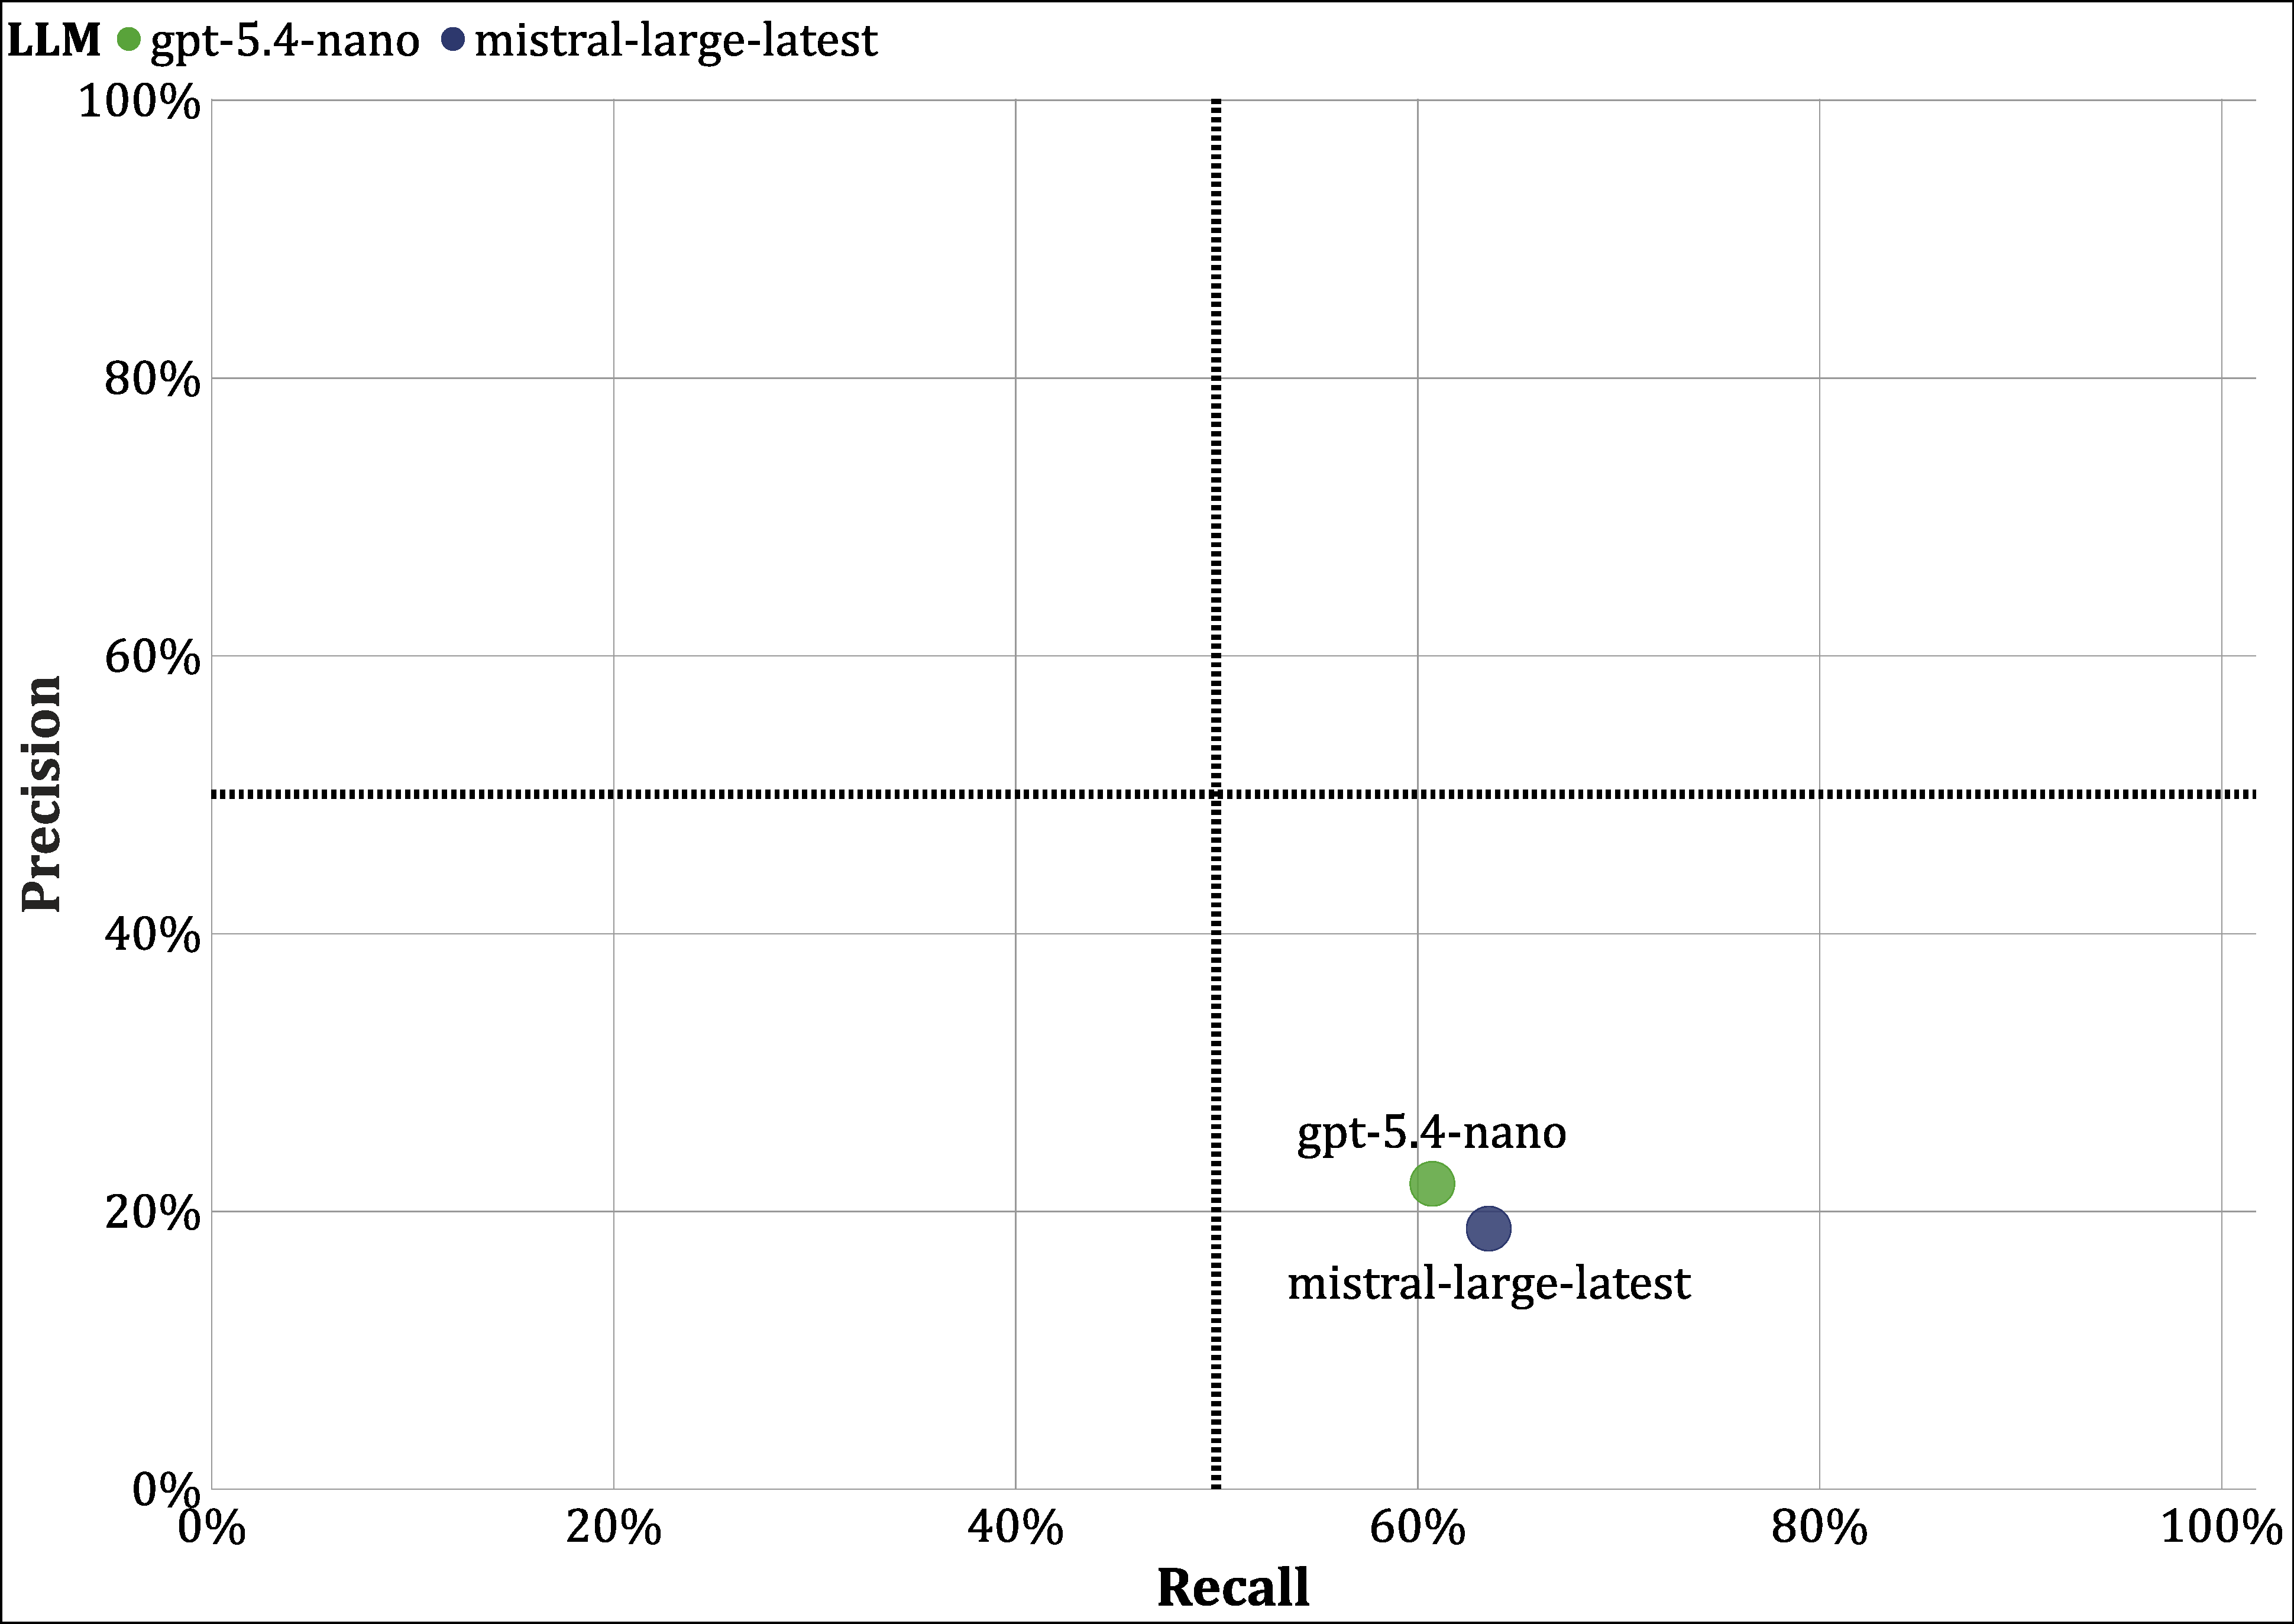
\includegraphics[width=0.8\textwidth]{res/graphs/pomer-recall-precision-hra.pdf}
    \caption{Bodový graf zobrazující recall a precision u~dokumentu Hra}
    \label{fig:pomer-recall-precision-hra}
\end{figure}

\subsection{Formalizace}
Tabulka \ref{tab:formalizace-vysledky} zobrazuje accuracy podle modelů pro oba dokumenty ve formalizační fázi. V~této fázi se modelům dařilo výrazně lépe formalizovat požadavky (fáze 2) než je extrahovat (fáze 1), kromě modelu \verb"llama3.2:latest", který má ze všech modelů nejmenší accuracy. 

Čísla v~závorce za dokumenty označují \textbf{počet správných formalizací z~počtu ohodnocených formalizací}. Z~důvodu velké časové náročnosti nebyly v~rozhraní Textractor Studio vyhodnoceny všechny vygenerované formalizace u~dokumentu NIS, což je třeba brát v~potaz u~jejich accuracy. Tabulka \ref{tab:formalizace-pocty} ukazuje počty ohodnocených formalizací pro oba dokumenty a pro všechny použité modely. Pro dokument NIS bylo ohodnoceno sekvenčně 527 požadavků z~celkem 1968.

\begin{table}
\catcode`-=12
\centering
\caption{Accuracy ve formalizační fázi podle modelů}
\label{tab:formalizace-vysledky}
\begin{tabularx}{\textwidth}{X || r r r}
\hline\hline
\multirow{2}{*}{\textbf{Dokument}} & \multicolumn{3}{c}{\textbf{Accuracy (správně/celkem)}} \\
\cline{2-4}
 & \texttt{gpt-5.4-nano} & \texttt{mistral-large-latest} & \texttt{llama3.2:latest} \\
\hline
NIS & 88,64\,\% (234/264) & 87,83\,\% (231/263) & --- \\
Hra & 90,65\,\% (97/107)  & 85,05\,\% (91/107)  & 38,32\,\% (41/107) \\
\hline\hline
\end{tabularx}
\end{table}

\begin{table}
\catcode`-=12
\centering
\caption{Počty ohodnocených formalizací podle dokumentů a modelů}
\label{tab:formalizace-pocty}
\begin{tabularx}{\textwidth}{X || Xrr}
\toprule
\toprule
\textbf{Dokument} & \textbf{Model} & \textbf{Celkem} & \textbf{Ohodnoceno} \\
\midrule
\multirow{4}{*}{NIS}
& \texttt{gpt-5.4-nano} & 984 & 264 \\
& \texttt{mistral-large-latest} & 984 & 263 \\
& \textbf{Total} & \textbf{1968} & \textbf{527} \\
\midrule
\multirow{4}{*}{Hra}
& \texttt{gpt-5.4-nano} & 107 & 107 \\
& \texttt{mistral-large-latest} & 107 & 107 \\
& \texttt{llama3.2:latest} & 107 & 107 \\
& \textbf{Celkem} & \textbf{321} & \textbf{321} \\
\midrule
\multirow{4}{*}{\textbf{Celkem}}
& \texttt{gpt-5.4-nano} & 1091 & 371 \\
& \texttt{mistral-large-latest} & 1091 & 370 \\
& \texttt{llama3.2:latest} & 107 & 107 \\
& \textbf{Celkem} & \textbf{2289} & \textbf{848} \\
\bottomrule
\bottomrule
\end{tabularx}
\end{table}


Obrázky \ref{fig:spravne-spatne-hra} a \ref{fig:spravne-spatne-nis} ukazují grafy s~počty správně a chybně formalizovaných požadavků použitých modelů pro dokumenty Hra a NIS. Pro dokument NIS existuje více správně extrahovaných požadavků, což je způsobeno jeho velikostí.
        

\begin{figure}[p]
    \centering
    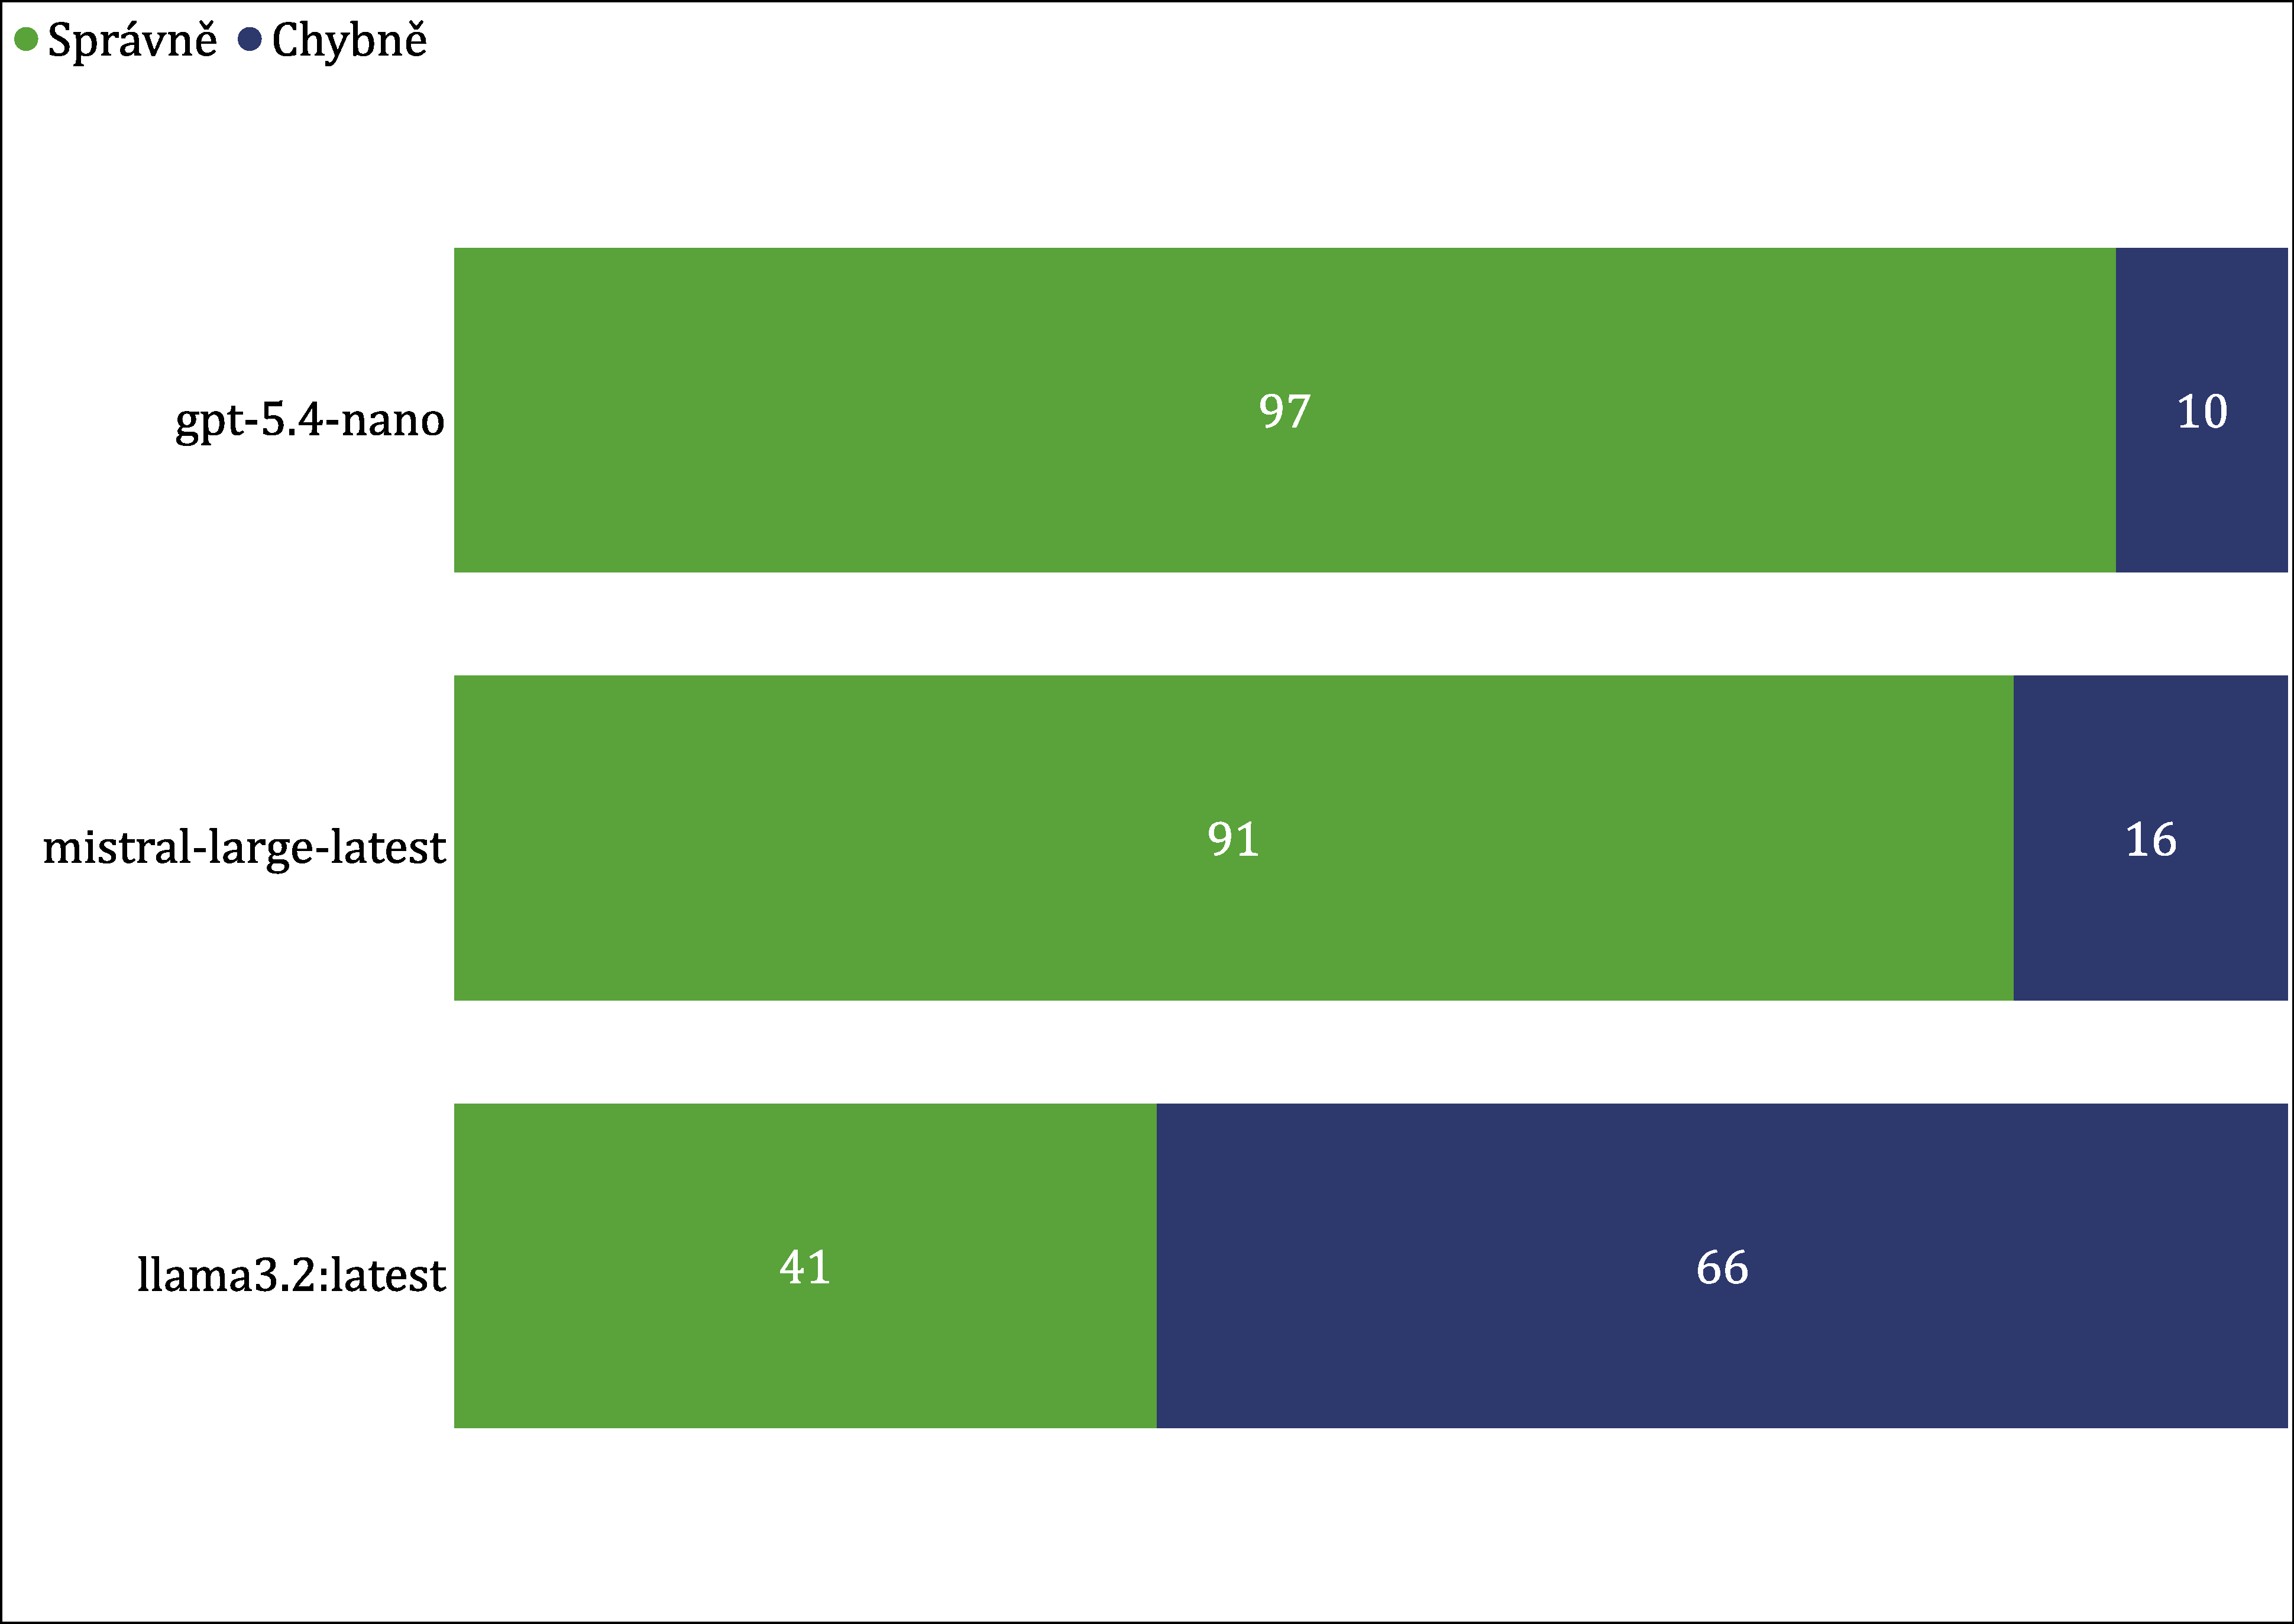
\includegraphics[width=0.8\textwidth]{res/graphs/spravne-spatne-hra.pdf}
    \caption{Počet správných a špatných formalizací podle modelů pro dokument Hra}
    \label{fig:spravne-spatne-hra}
\end{figure}

\begin{figure}[p]
    \centering
    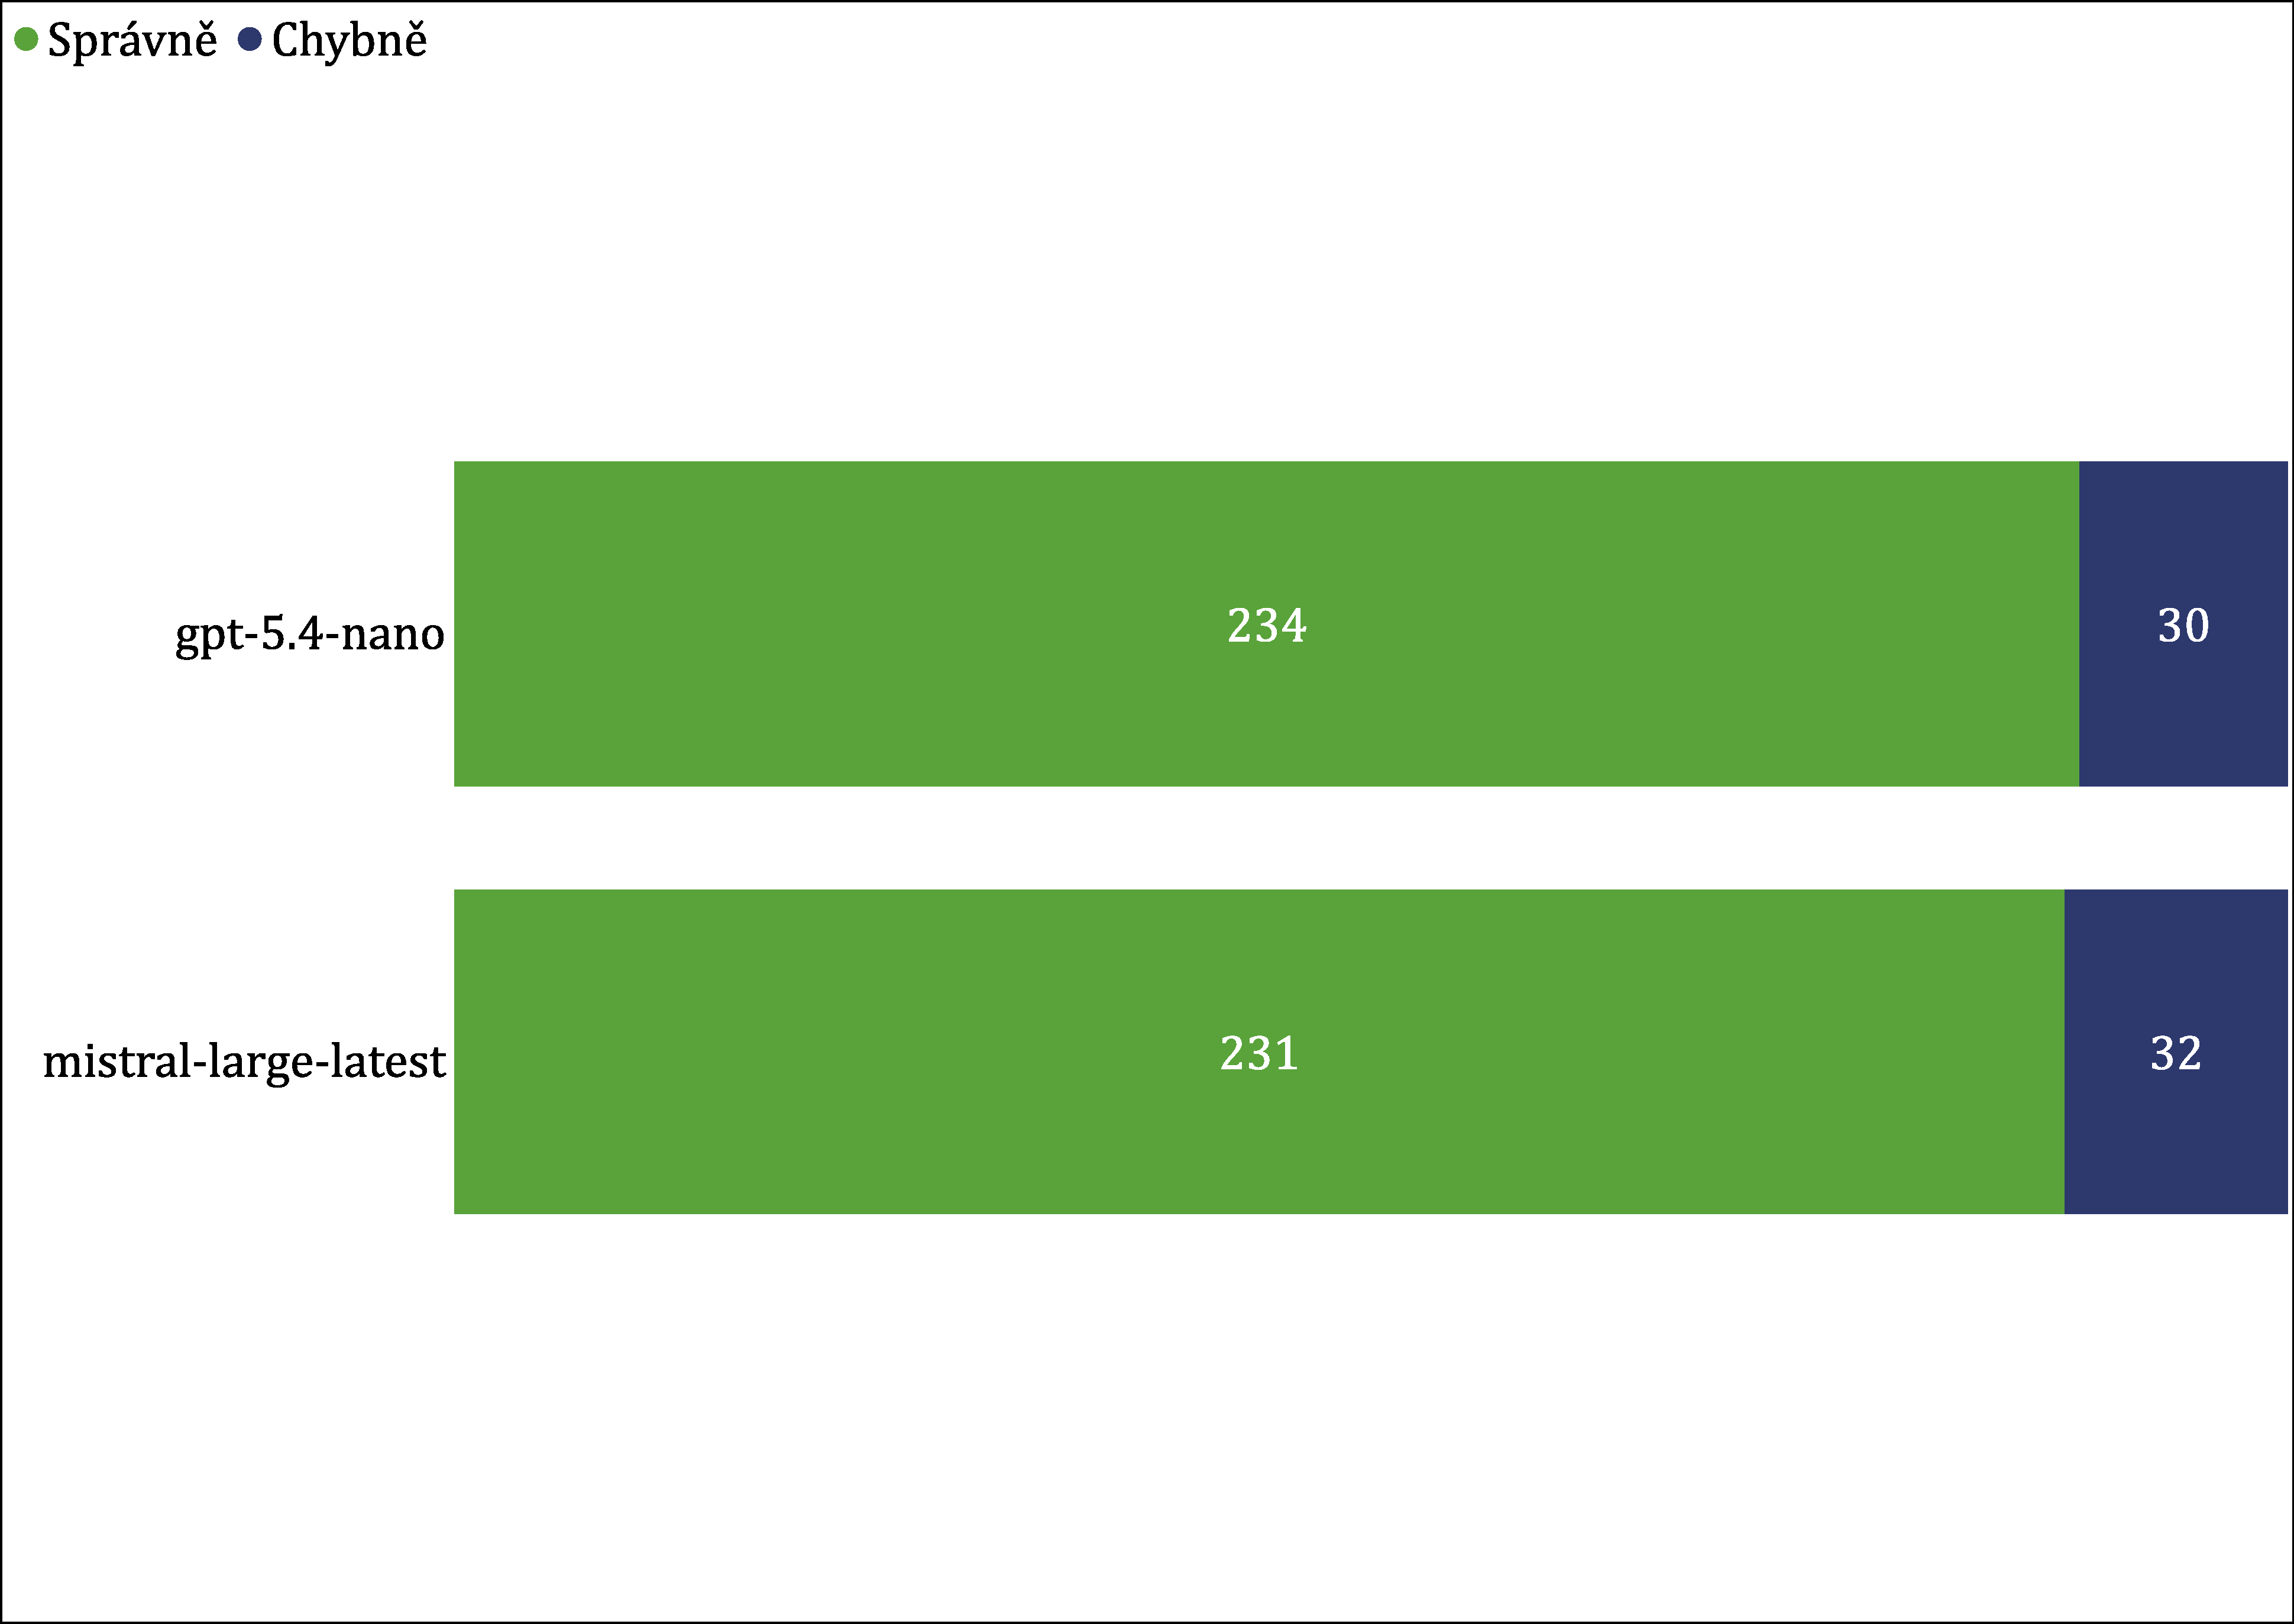
\includegraphics[width=0.8\textwidth]{res/graphs/spravne-spatne-nis.pdf}
    \caption{Počet správných a špatných formalizací podle modelů pro dokument NIS}
    \label{fig:spravne-spatne-nis}
\end{figure}

\clearpage
\section{Poměr ceny a kvality}
Obrázek \ref{fig:cena-f1-extrakce-hra} ukazuje v~bodovém grafu poměr průměrné ceny extrakce dokumentu a kvality (pomocí F1 skóre). 


\begin{figure}[h!]
    \centering
    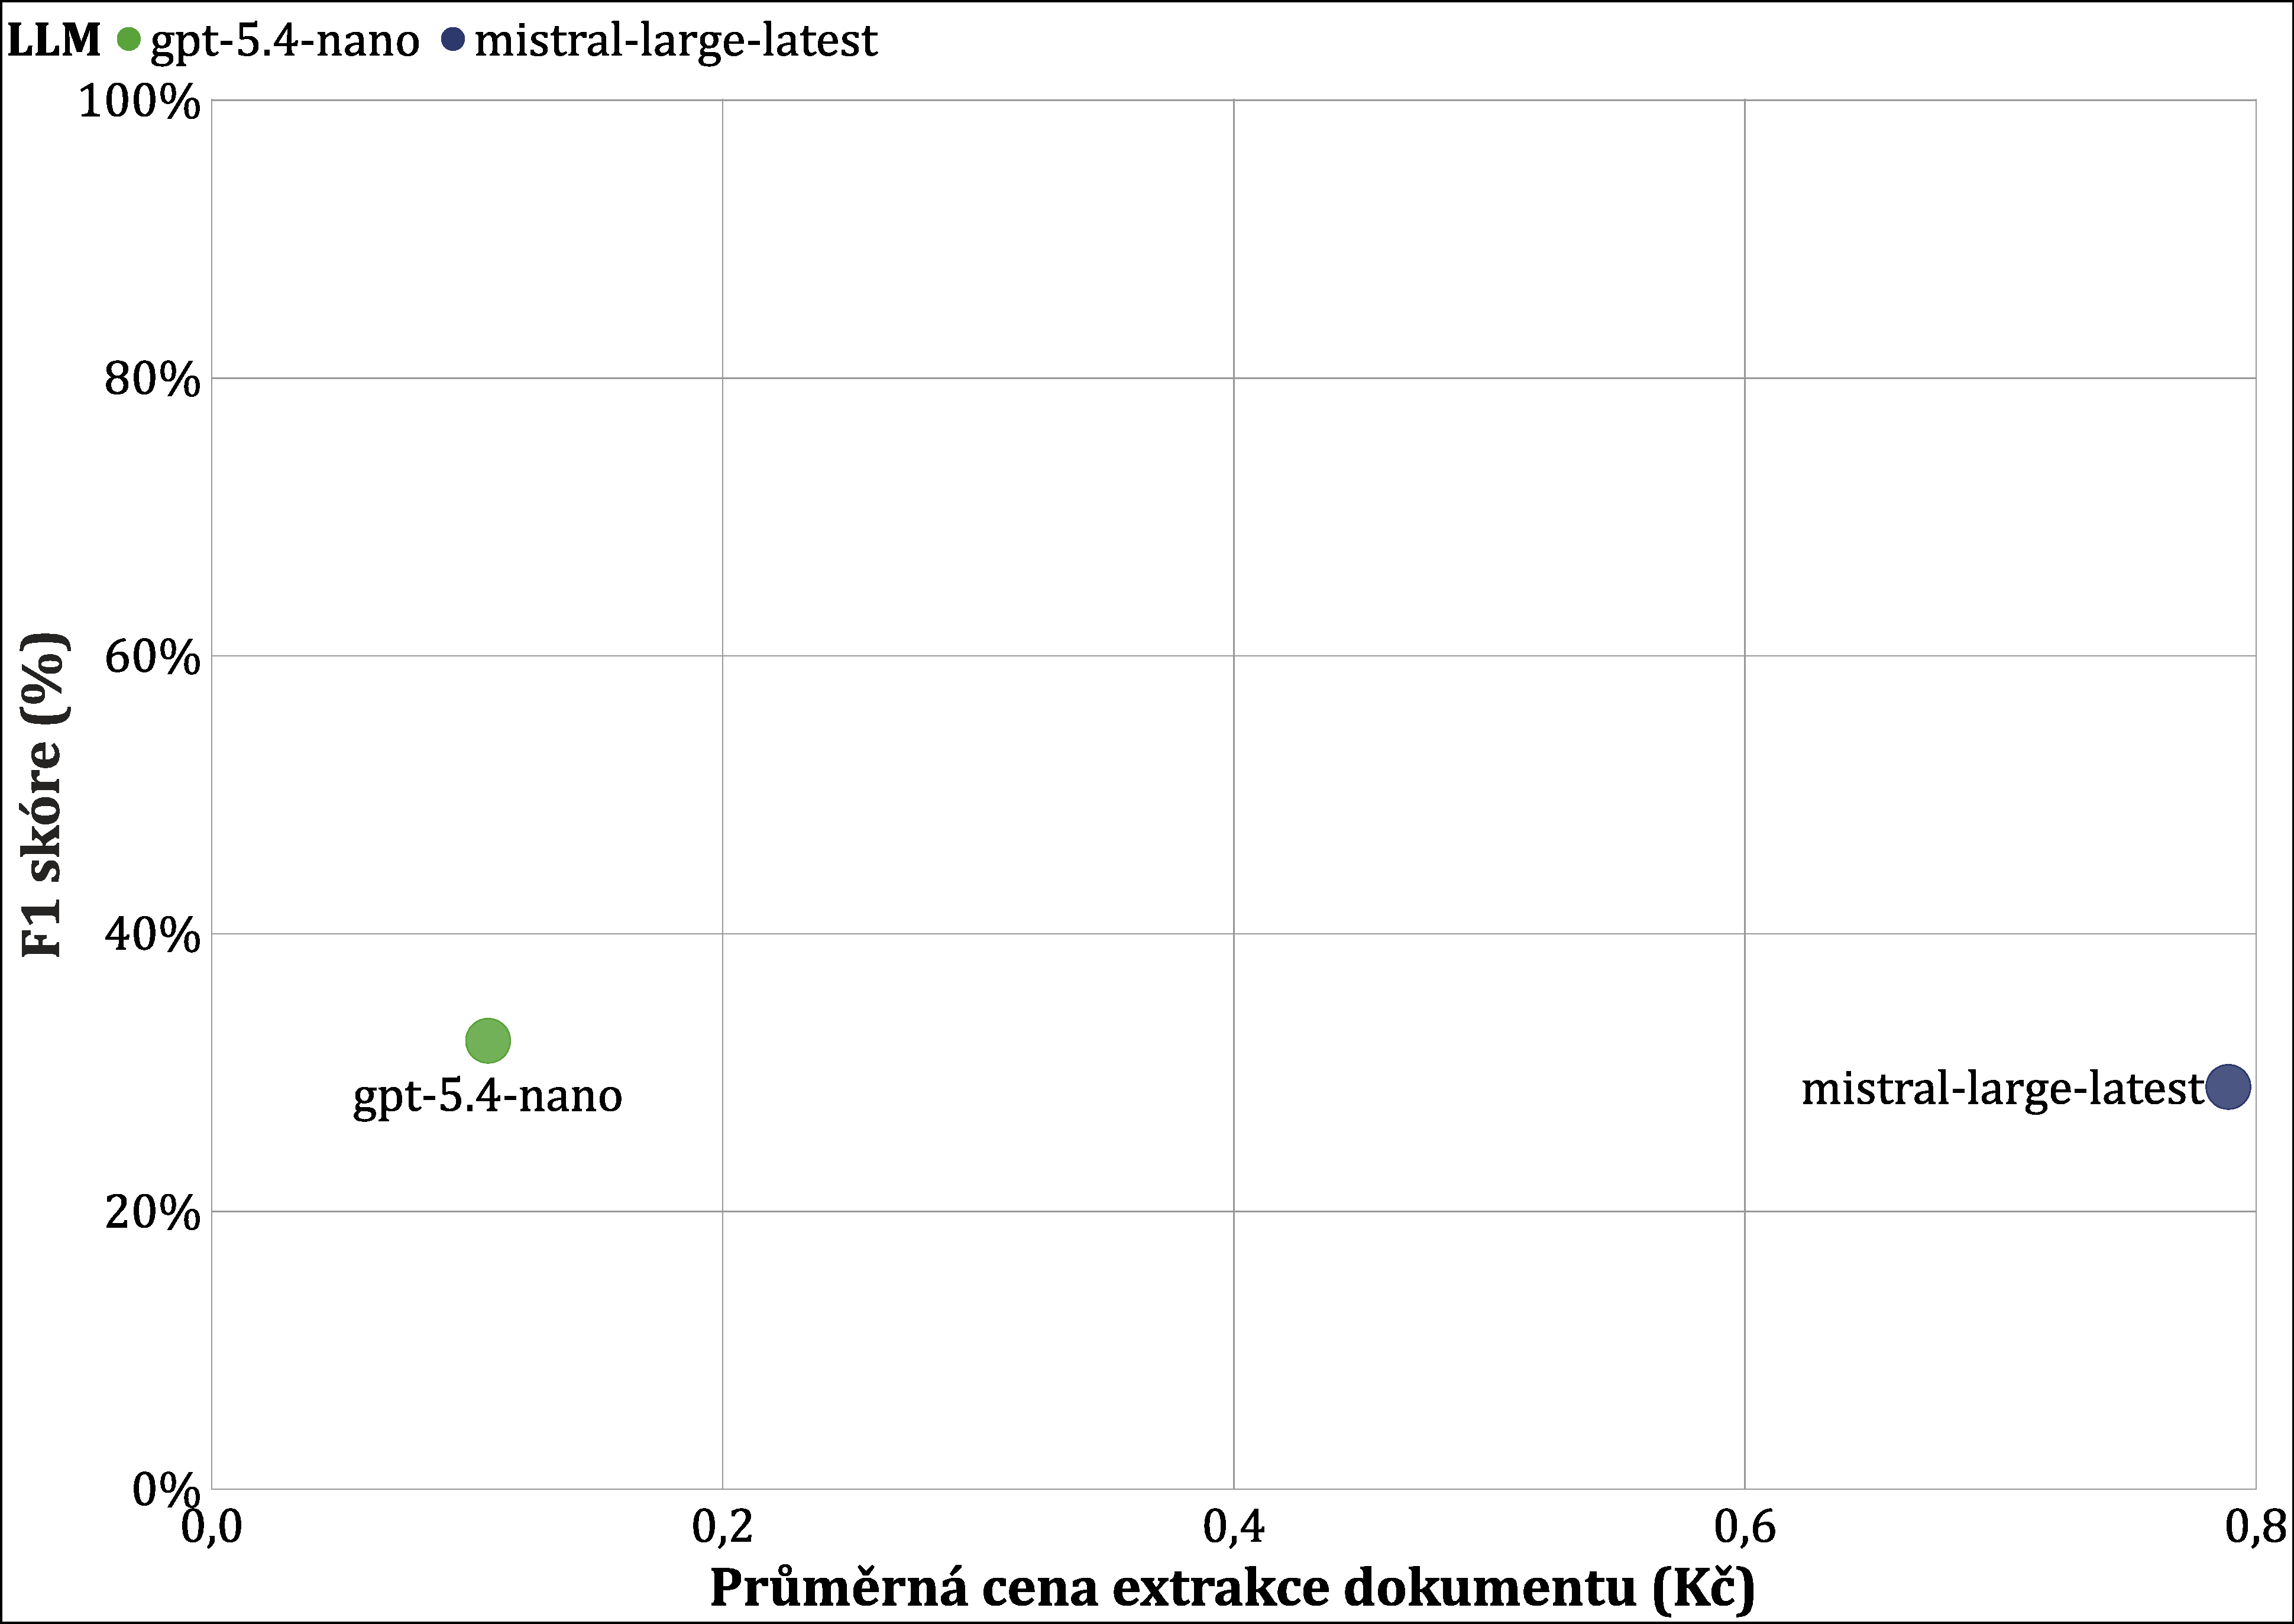
\includegraphics[width=0.8\textwidth]{res/graphs/cena-f1-extrakce-hra.pdf}
    \caption{Bodový graf zobrazující poměr F1 skóre recall a průměrné ceny u~dokumentu Hra}
    \label{fig:cena-f1-extrakce-hra}
\end{figure}

Na obrázku \ref{fig:cena-accuracy-formalizace-nis} je zobrazeno srovnání průměrné ceny formalizace jednoho požadavku a accuracy pro dokument NIS. Na obrázku \ref{fig:cena-accuracy-formalizace-hra} pro dokument Hra se stejným srovnáním přibyl model \verb"llama3.2:latest", který je sice levný, ale výrazně horší v~accuracy oproti ostatním modelům.

\begin{figure}[p]
    \centering
    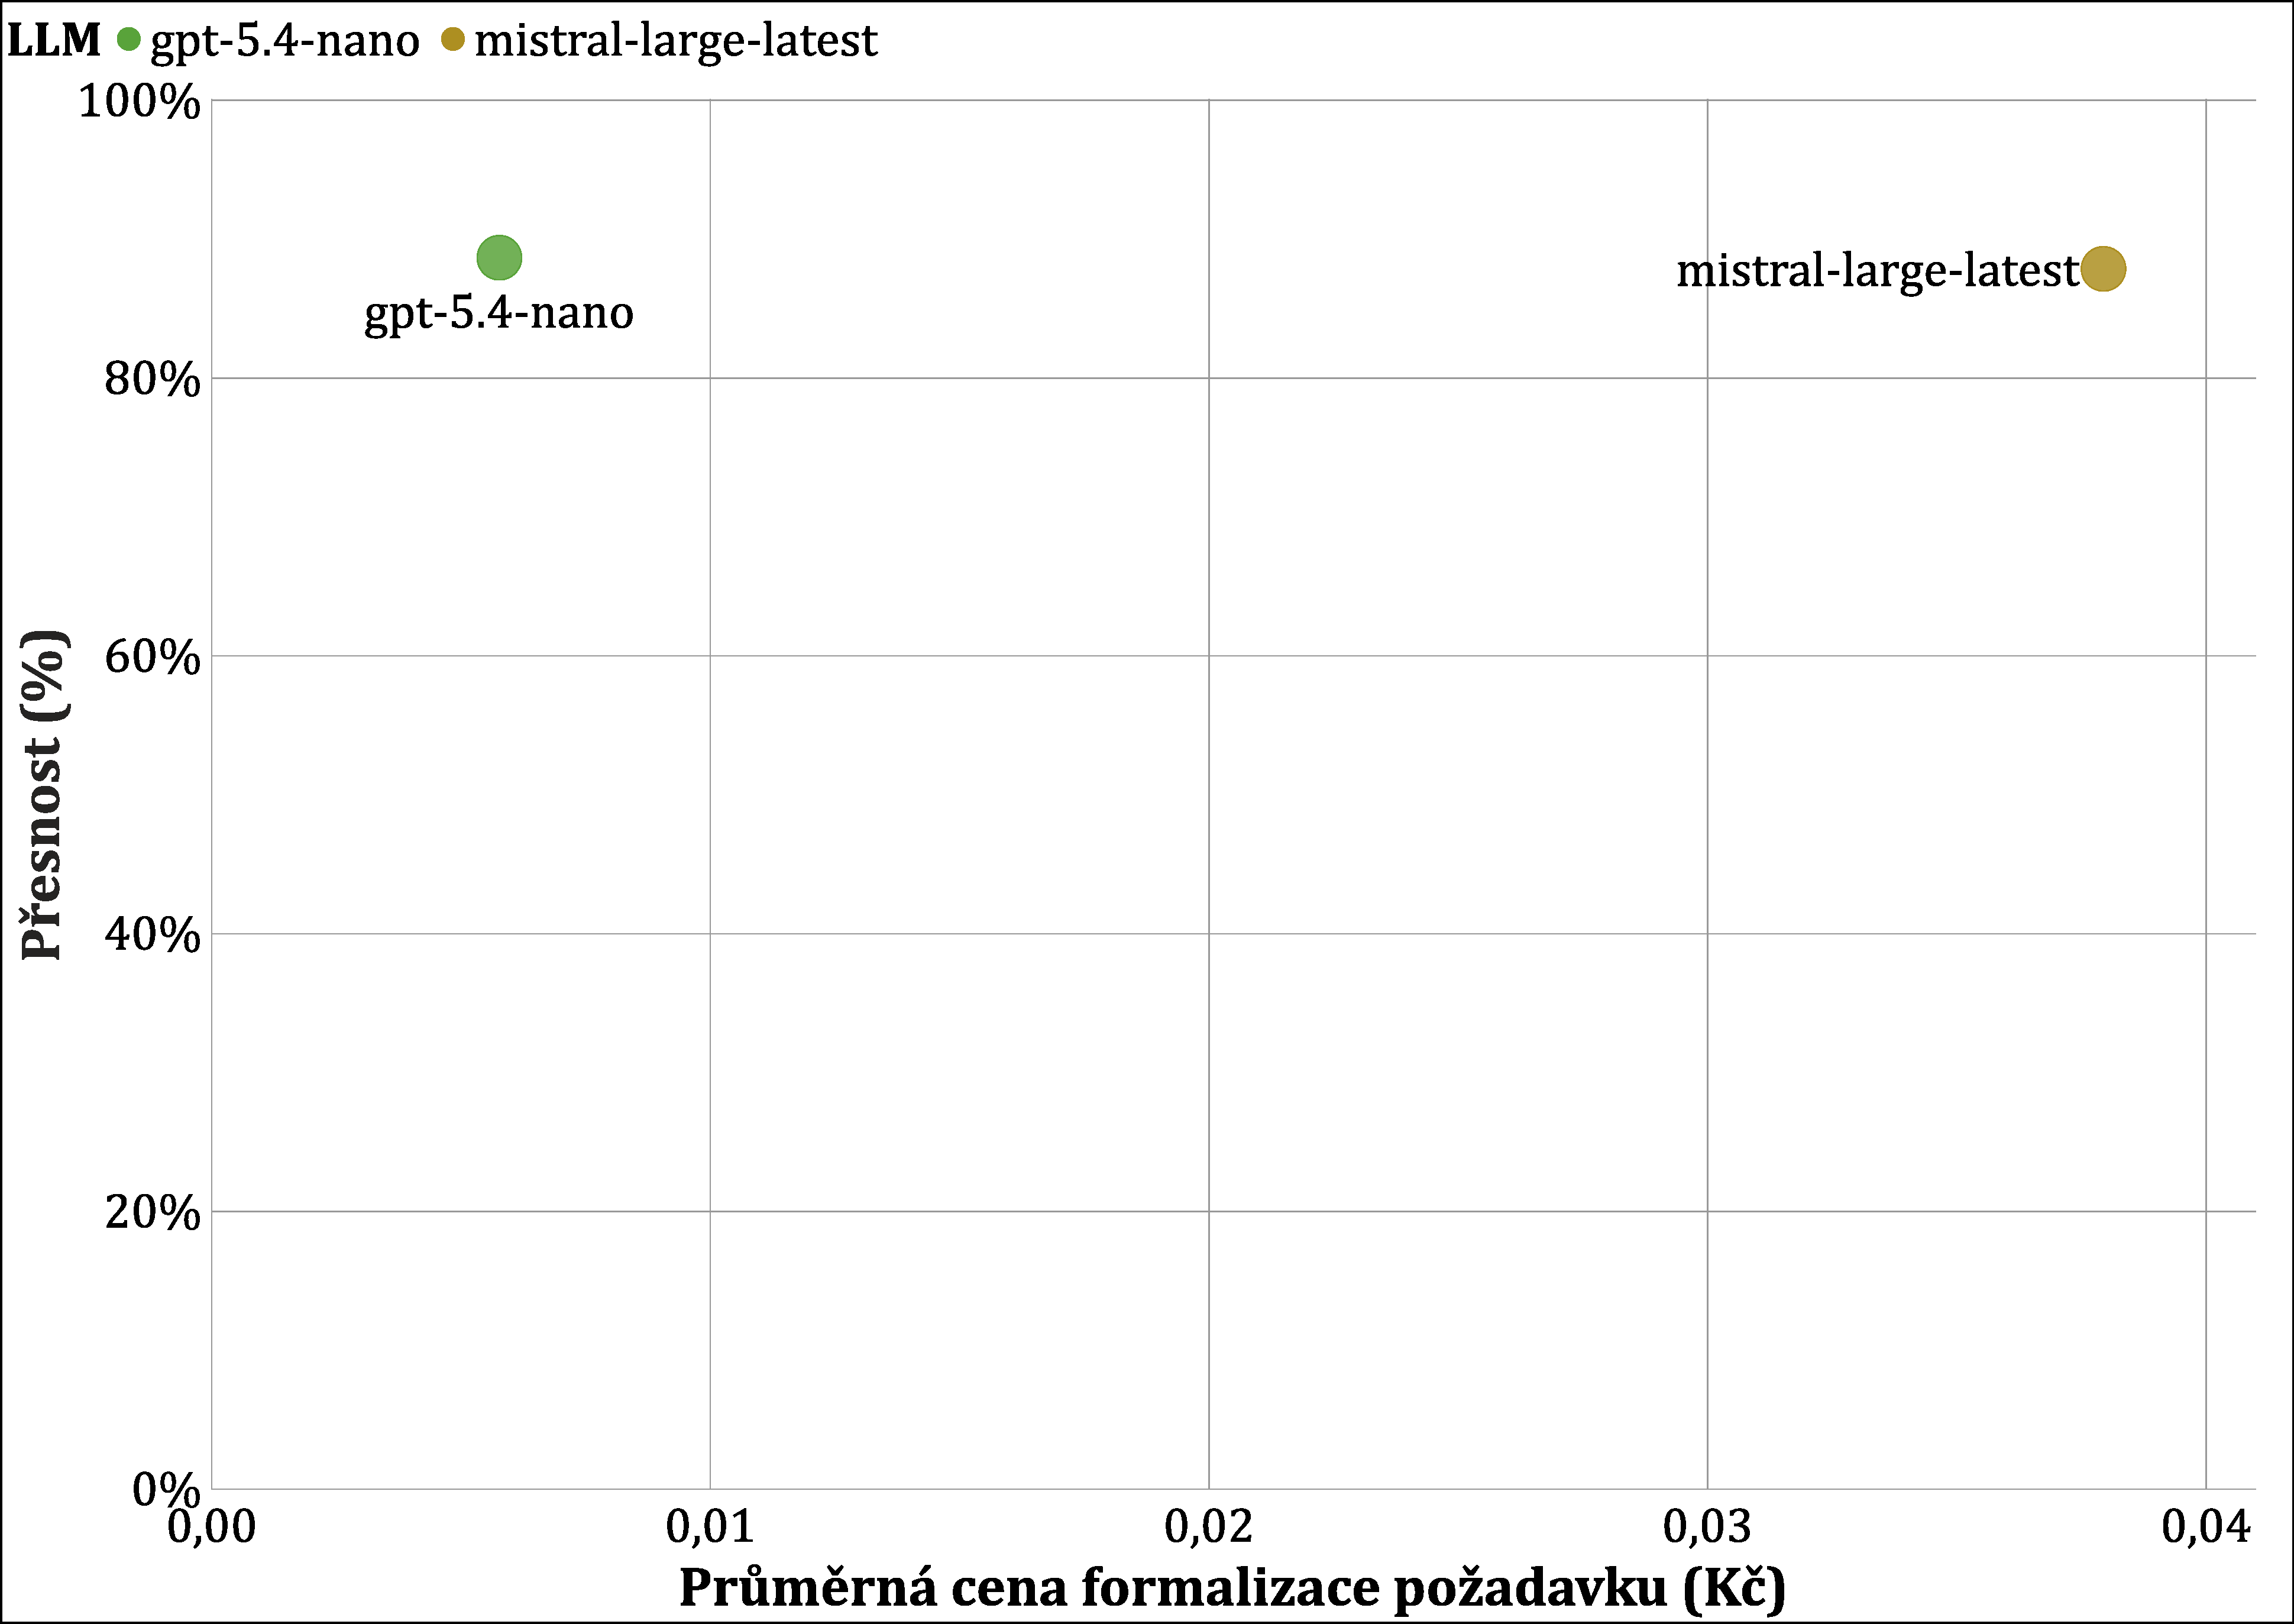
\includegraphics[width=0.8\textwidth]{res/graphs/cena-accuracy-formalizace-nis.pdf}
    \caption{Bodový graf zobrazující poměr accuracy a průměrné ceny u~dokumentu NIS}
    \label{fig:cena-accuracy-formalizace-nis}    
\end{figure}

\begin{figure}[p]
    \centering
    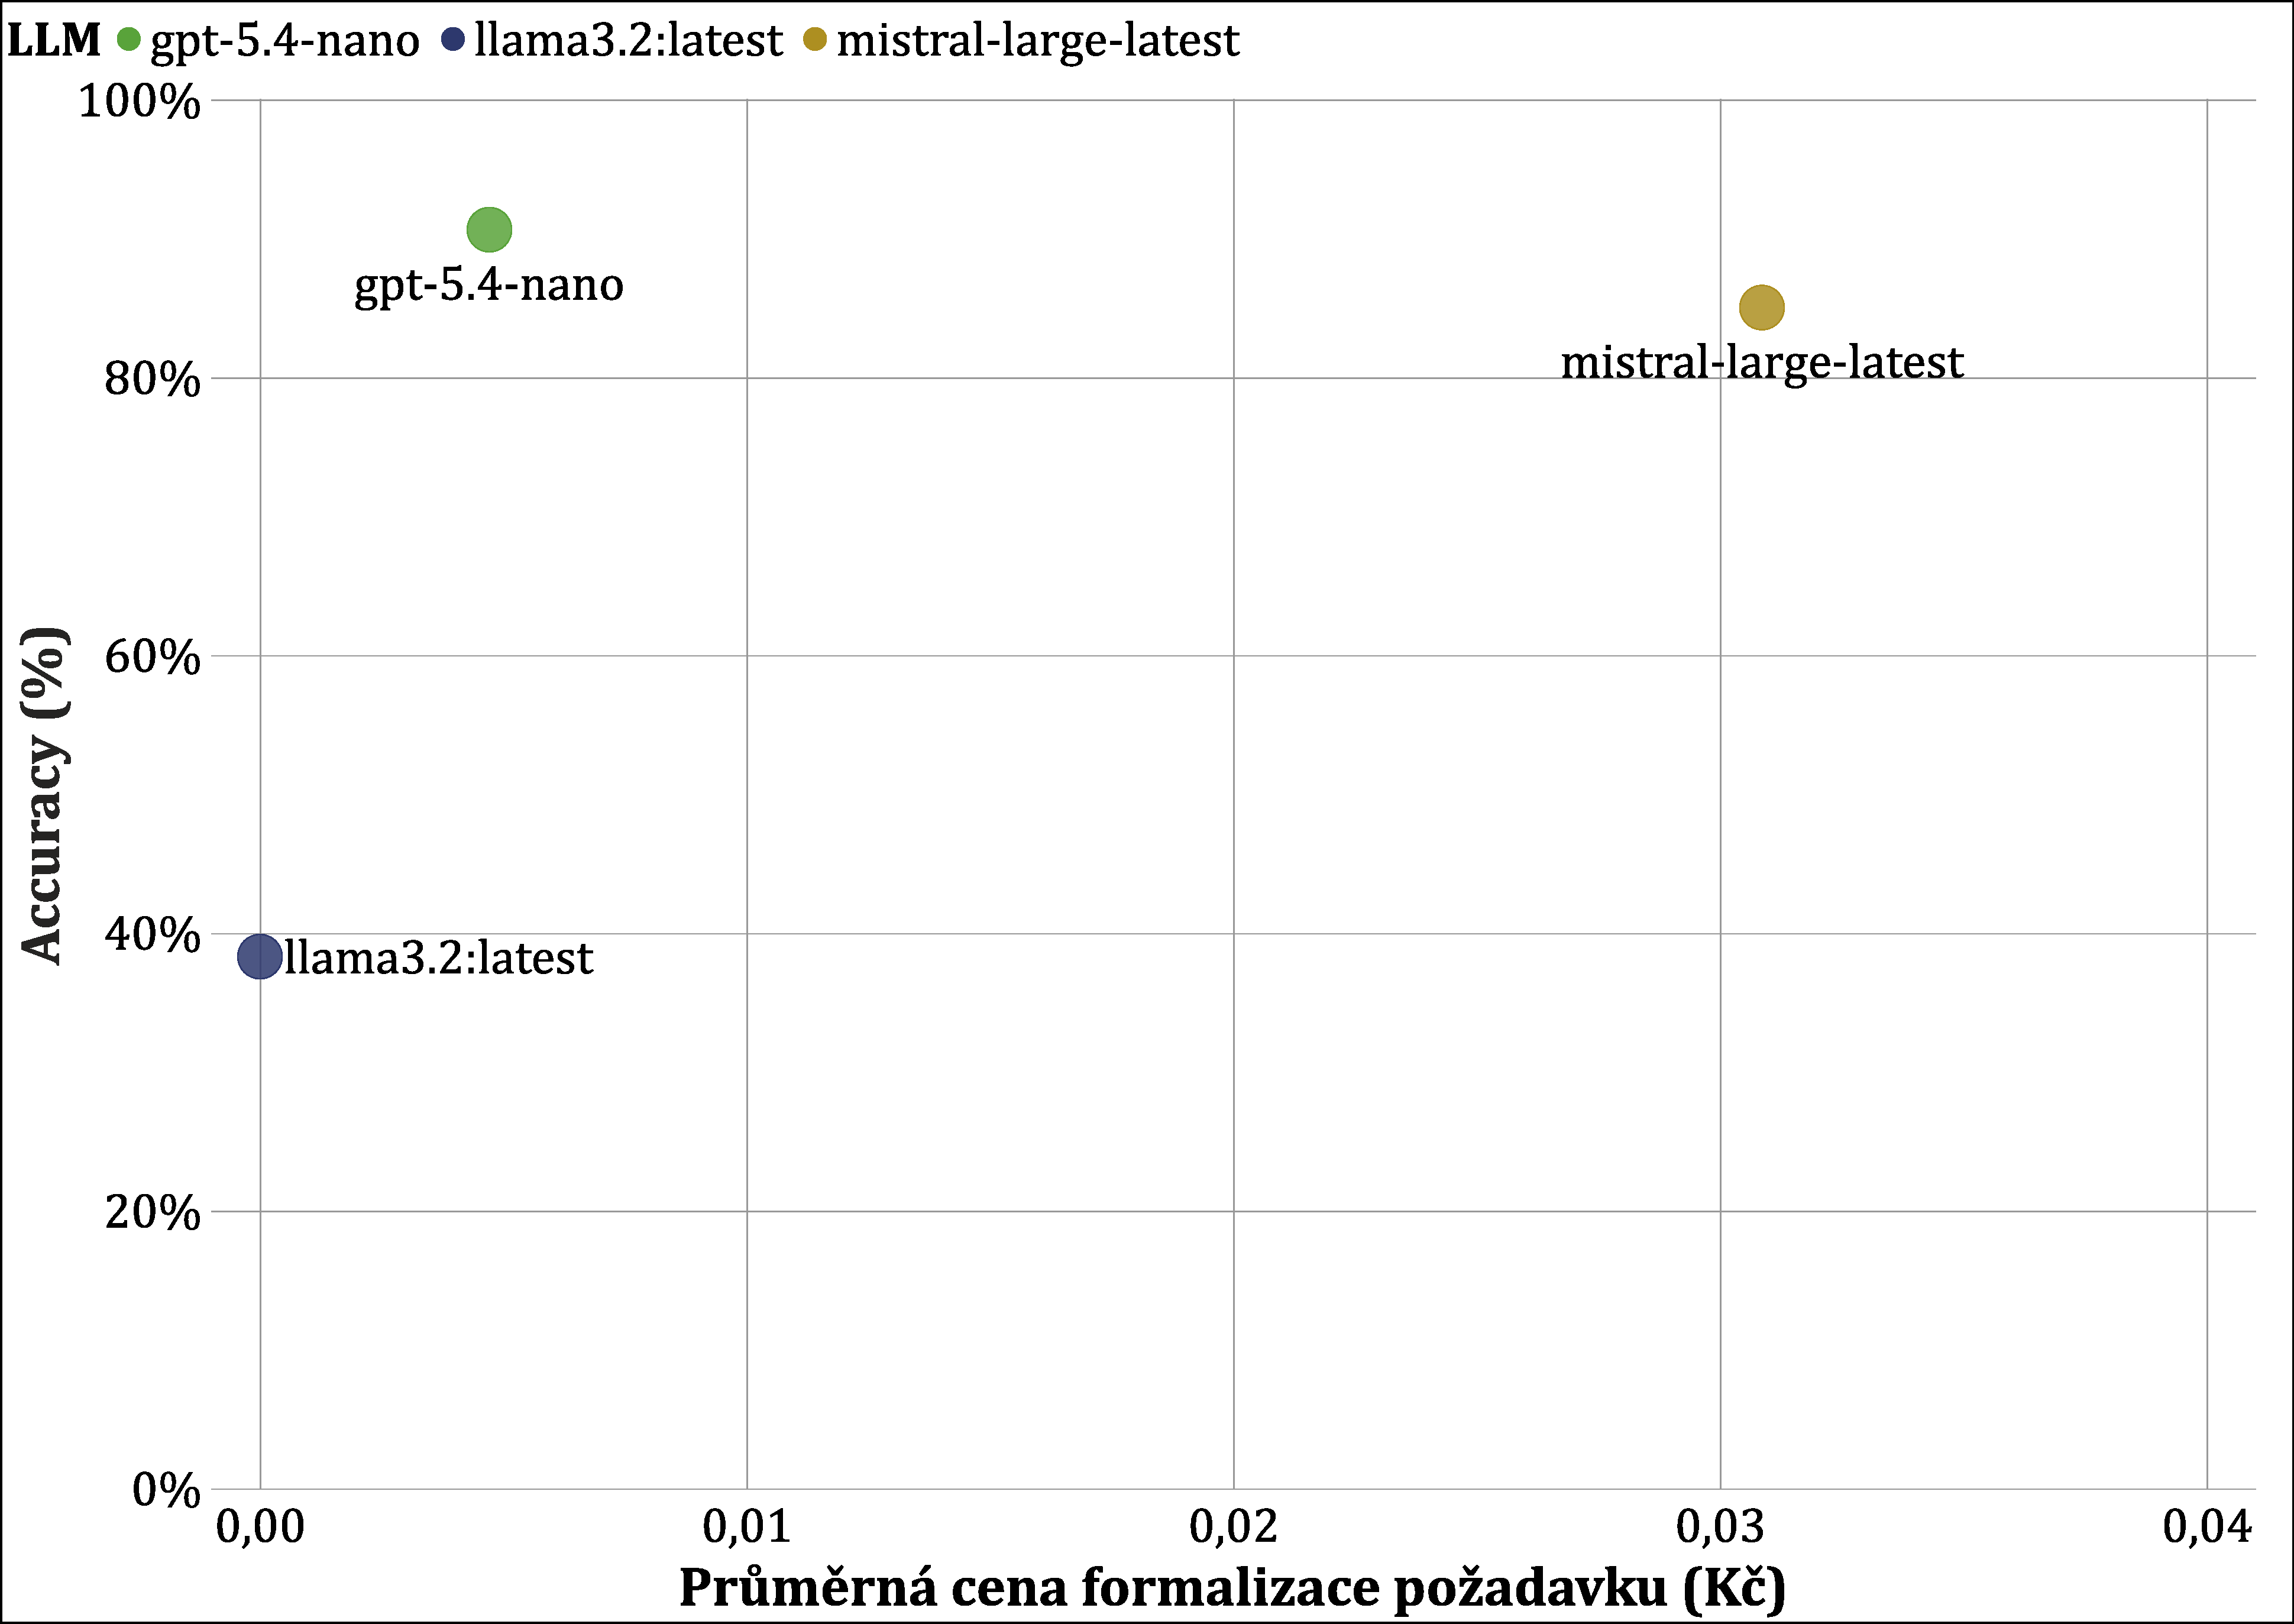
\includegraphics[width=0.8\textwidth]{res/graphs/cena-accuracy-formalizace-hra.pdf}
    \caption{Bodový graf zobrazující poměr accuracy a průměrné ceny u~dokumentu Hra}
    \label{fig:cena-accuracy-formalizace-hra}
\end{figure}

\clearpage
\section{Časté chyby modelů}
Velké jazykové modely se dopouštěly při extrakci i formalizaci častých chyb, které byly pozorovány při hodnocení v~rozhraní Textractor Studio. Tyto chyby jsou popsány v~tabulce \ref{tab:caste-chyby}. První sloupec reprezentuje typ chyby, kde písmeno reprezentuje fázi, ve které se chyba vyskytovala -- \uv{E} pro extrakční fázi a \uv{F} pro formalizační fázi. Číslo za daným písmenem znamená označení chyby.

\newcounter{errnum}
\newcommand{\echyba}[1]{E\stepcounter{errnum}\theerrnum & #1 \\}
\newcommand{\fchyba}[1]{F\stepcounter{errnum}\theerrnum & #1 \\}

\setcounter{errnum}{0}
\begin{center}
\begin{longtable}[h!]{p{0.05\textwidth}||p{0.95\textwidth}}
\caption{Přehled častých chyb LLM u~extrakční a formalizační fáze}
\label{tab:caste-chyby}\\
\toprule[1.5pt]
& \textbf{Popis chyby}\\
\midrule
\endfirsthead
\multicolumn{2}{c}{\tablename{}~\thetable{}
    \textit{(pokračování z~předchozí stránky)}}\\
\midrule
 & \textbf{Popis chyby}\\
\midrule
\endhead
\midrule
\multicolumn{2}{r}{\textit{(tabulka pokračuje na další stránce)}}\\
\endfoot
\bottomrule[1.5pt]
\endlastfoot
\echyba{I~přes výslovný zákaz v~systémové zprávě LLM nedodávají kontext k~požadavku (ani ve formě nadpisů, ani jinak). Toto poté způsobuje zneplatnění požadavku, protože z~něj nelze pochopit širší kontext. Například věta \uv{Možnost volby formátu A4 a A5.} neříká, v~jaké sekci systému se to má vyskytovat, nebo kde tento formát vybrat.}
\echyba{Seznamy s~odrážkami jsou rozdělovány jako různé požadavky. Výsledný text jednoho požadavku pak nepředává potřebnou informaci.}
\echyba{Zkopírování části požadavku bez dodatečných informací, které do něj jasně patří, i přes to, že jsou součástí nějaké věty (často výrazy \uv{\dots např. \dots} nebo \uv{\dots na odkaze \dots}).}
\echyba{Zkopírování jen části souvětí.}
\echyba{Zkopírování věty obsahující požadavek a ignorování dodatečných závorek pro upřesnění.}
\fchyba{Modely překládají text do anglického jazyka, i přes výslovný zákaz překládání textu do jiného jazyka v~systémové zprávě.\textsuperscript{*} }
\fchyba{Objevují se halucinace ve formalizovaných textech, zpravidla pokud model usoudí, že nemá dostatek kontextu pro doplnění.}
\fchyba{Model \verb"llama3.2:latest" při některých požadavcích místo reálné formalizace použije přesný příklad uvedený v~systémové zprávě.}
\fchyba{Model \verb"llama3.2:latest" většinu textu některých požadavků neformalizuje, jen z~nich přepíše klíčové slovo.}
\fchyba{Při formalizaci modely často ignorují webové odkazy.}
\fchyba{Pokud extrahovaný text obsahuje nadpis, modely ho většinou nerozpoznají a soustředí se na vlastnosti v~požadavku, což v~některých případech nevadí, pokud tyto vlastnosti obsahují dostatečný kontext a lze z~nich pochopit účel požadavku.}
\fchyba{Model \verb"mistral-large-latest" někdy identifikuje náhodná čísla jako kvantifikovatelná data, i když nesouvisí s~požadavkem.}
\fchyba{Při formalizaci kvantifikovatelných dat LLM někdy nepřidá dodatečnou informaci k~parametru jednotky. Například u~informace \uv{\dots minimálně 10 let.} může být parametr jednotky jen \uv{let}.\textsuperscript{*}}
\fchyba{Modely si mohou spléct uvedení příkladu (\uv{\dots např. \dots}) v~požadavku jako jedinou možnost, jak danou činnost vykonat, nikoliv jako příklad.}

\end{longtable}
\begin{flushleft}
\footnotesize $^*$ Toto chování není bráno jako chyba při vyhodnocení v~rozhraní Textractor Studio z~důvodu velmi častého výskytu a nerelevanci k~extrakci/formalizaci informací jinak obsažených v~požadavku.
\end{flushleft}
\end{center}

\clearpage
\section{Shrnutí}
Z~informací v~této kapitole vyšel nejlépe model \verb"gpt-5.4-nano", i přes to, že model \verb"mistral-large-latest" disponuje vyšším recall u~dokumentu Hra. Nedokázal ale v~první fázi zpracovat dokument NIS, s~čímž si naopak model \verb"gpt-5.4-nano" poradit dokázal.

Pokud by ruční extrakci a formalizaci vykonával člověk, strávil by na tom o~959,1 minut déle, než model \verb"gpt-5.4-nano". Tabulka \ref{tab:cena-rucni-vs-modely} ukazuje srovnání cen a časů práce člověka oproti práci tohoto modelu v~extrakční i formalizační fázi v~obou dokumentech. Pokud je tedy definováno ocenění ruční práce extrakce a formalizace člověka jako 250 Kč za hodinu, při použití tohoto modelu \textbf{se ušetří 4 117,59 Kč}. \textbf{Pro tyto výpočty byly použity přibližné časy ruční extrakce a formalizace popsány v~sekci \ref{sec:vyhodnoceni-srovnani-casu}.}

Je ale důležité zmínit, že \textbf{požadované F1 skóre a accuracy nemusí být pro určité úkoly dostačující.}


\begin{table}[h!]
\centering
\caption{Srovnání cen a časů práce člověka proti práci modelu \texttt{gpt-5.4-nano}}
\label{tab:cena-rucni-vs-modely}
\begin{tabularx}{\textwidth}{>{\raggedright\arraybackslash}X|
                              >{\raggedleft\arraybackslash}X}
\hline\hline
\textbf{Celková cena člověka}          & 4 125,00 Kč          \\
\textbf{Celková cena modelu}           & 7,41 Kč              \\
\textbf{Celkový čas modelu}            & 30,90 min            \\
\textbf{Celkový čas člověka}           & 990 min              \\
\textbf{Ušetřený čas díky modelu}      & \textbf{959,10 min}  \\
\textbf{Ušetřené peníze díky modelu}   & \textbf{4 117,59 Kč} \\
\hline\hline
\end{tabularx}
\end{table}


\chapter{Závěr}
Tato práce prozkoumala, jak kvalitně dokážou velké jazykové modely extrahovat a formalizovat data ze specifikací softwarových požadavků. Nejlepší z~porovnávaných modelů podle kvality a ceny je \verb"gpt-5.4-nano", který dokázal zpracovat oba testované dokumenty. Další vyzkoušené modely byly \verb"mistral-large-latest" pro obě fáze a \verb"llama3.2:latest" pro formalizační fázi. 

V~extrakční fázi dosáhl model \verb"gpt-5.4-nano" F1 skóre 29,32 \% pro delší dokument a 32,26 \% pro kratší dokument. Pro srovnání, model \verb"mistral-large-latest" dosáhl F1 skóre 28,94 \% na kratším dokumentu a delší nezpracoval. Tyto hodnoty byly ověřeny ručně oproti referenčním extrakcím a jsou pro produkční nasazení nedostatečné. Modely totiž často nedodávaly kontext nezbytný pro pochopení požadavku (například nadpis nebo okolní věty).

Ve formalizační fázi, která byla prováděna na jednotlivých extrahovaných požadavcích, dosáhly modely výrazně lepších výsledků. Accuracy modelu \verb"gpt-5.4-nano" se pohybovala mezi 88,64 \% a 90,65 \%, \verb"mistral-large-latest" mezi 85,05 \% a 87,83~\% a u~\verb"llama3.2:latest" dosahovala pouze 38,32 \%. Může být tedy vhodné některé LLM pro formalizaci využít, ale menší lokální modely se na tento úkol nehodí. Je však dobré zkontrolovat výstupy, například v~rozhraní Textractor Studio. Častou chybou modelů bylo domýšlení informací.

Vyvinutý nástroj je připraven pro budoucí rozšíření a další testování na různých dokumentech, nejen SRS. Výstupy jazykových modelů úzce souvisí se systémovou zprávou, která modelu předává instrukce pro daný úkol. Tuto zprávu je možné ladit pro určitý typ dokumentů a pozorovat, jak se výsledky podle těchto zpráv mění. Další možnost pro zlepšení výsledků může být rozdělení dokumentu a zpracování po menších částech, což by vyřešilo problém neschopnosti některých modelů (například \verb"mistral-large-latest") zpracovat příliš dlouhý text.

Grafické uživatelské rozhraní Textractor Studio bylo testováno pro evaluační režim, který používá ručně extrahované a formalizované požadavky. Další práce se může také zaměřit na vylepšení produkčního režimu, který nepracuje s~referenčními informacemi, ale pouze s~původními dokumenty.


\listoffigures
\listoftables
\listoflistings

\printbibliography

% == APPENDIX ==
\appendix
\chapter{ERA model databáze}\label{pril:era}
Následující stránka obsahuje obrázek \ref{fig:era} zobrazující ERA model databáze, kterou využívá program Textractor.

\begin{figure}[h!]
    \centering
    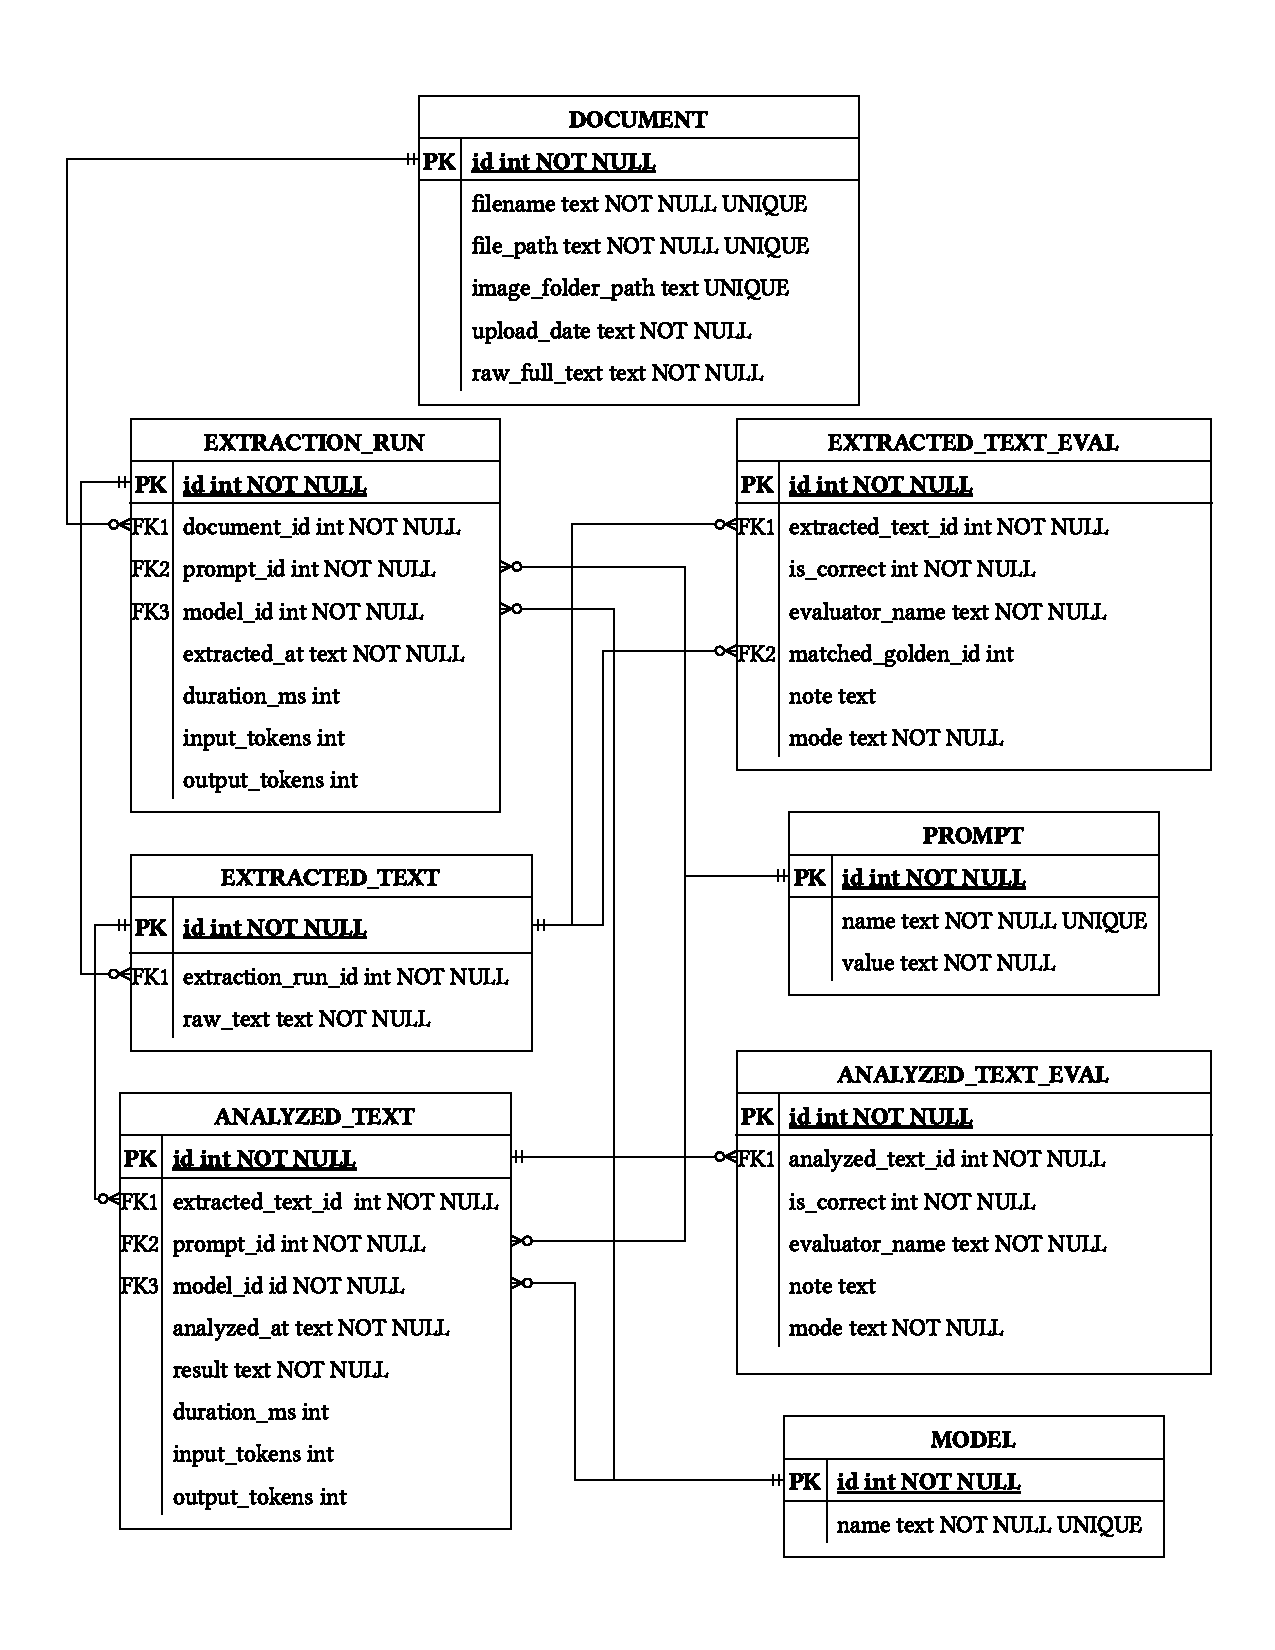
\includegraphics[width=\textwidth]{res/era.pdf}
    \caption{ERA model databáze pro extrakci dat z~projektové dokumentace}
    \label{fig:era}
\end{figure}

\chapter{Souborová struktura}\label{pril:soubory}
Tabulka \ref{tab:soubory} zobrazuje strukturu složek a spouštěcích skriptů programu Textractor.

\begin{table}[h!]
\centering
\caption{Základní struktura složek a souborů programu Textractor}
\label{tab:soubory}
\begin{tabular}{@{}ll@{}}
\toprule
\textbf{Soubor / složka} & \textbf{Popis} \\
\midrule \midrule
\filename"data/"                         & vstupní a výstupní data (PDF, databáze) \\
\quad\filename"golden_seed/"             & složka se zlatým datasetem \\
\quad\filename"raw_pdfs/"                & vstupní soubory pro extrakci \\
\quad\filename"extracted_images/"        & složka pro ukládání obrázků \\
\quad\filename"database.db"              & soubor s~databází \\
\filename"logs/"                         & soubory se záznamy běhu \\
\filename"src/"                          & zdrojové kódy aplikace \\
\quad\filename"database/"                & správa databáze \\
\quad\filename"documents/"               & načítání a zpracování dokumentů \\
\quad\filename"gui/"                     & komponenty grafického rozhraní \\
\quad\filename"llms/"                    & rozhraní pro komunikaci s~LLM \\
\quad\filename"pipeline/"                & skripty pro extrakci a formalizaci \\
\quad\filename"utils.py"                 & pomocné funkce \\
\filename"gui.py"                        & spouštěcí skript GUI \\
\filename"textractor.py"                 & vstupní bod programu \\
\filename"requirements.txt"              & seznam závislostí \\
\filename"setup.bat" / \filename"setup.sh" & instalační skripty \\
\bottomrule
\end{tabular}
\end{table}

\chapter{Diagram tříd databázových repozitářů}\label{pril:cls_db}
Následující stránka obsahuje obrázek \ref{fig:cls_db} diagramu tříd databázových repozitářů programu Textractor.

\begin{landscape}
    \begin{figure}
        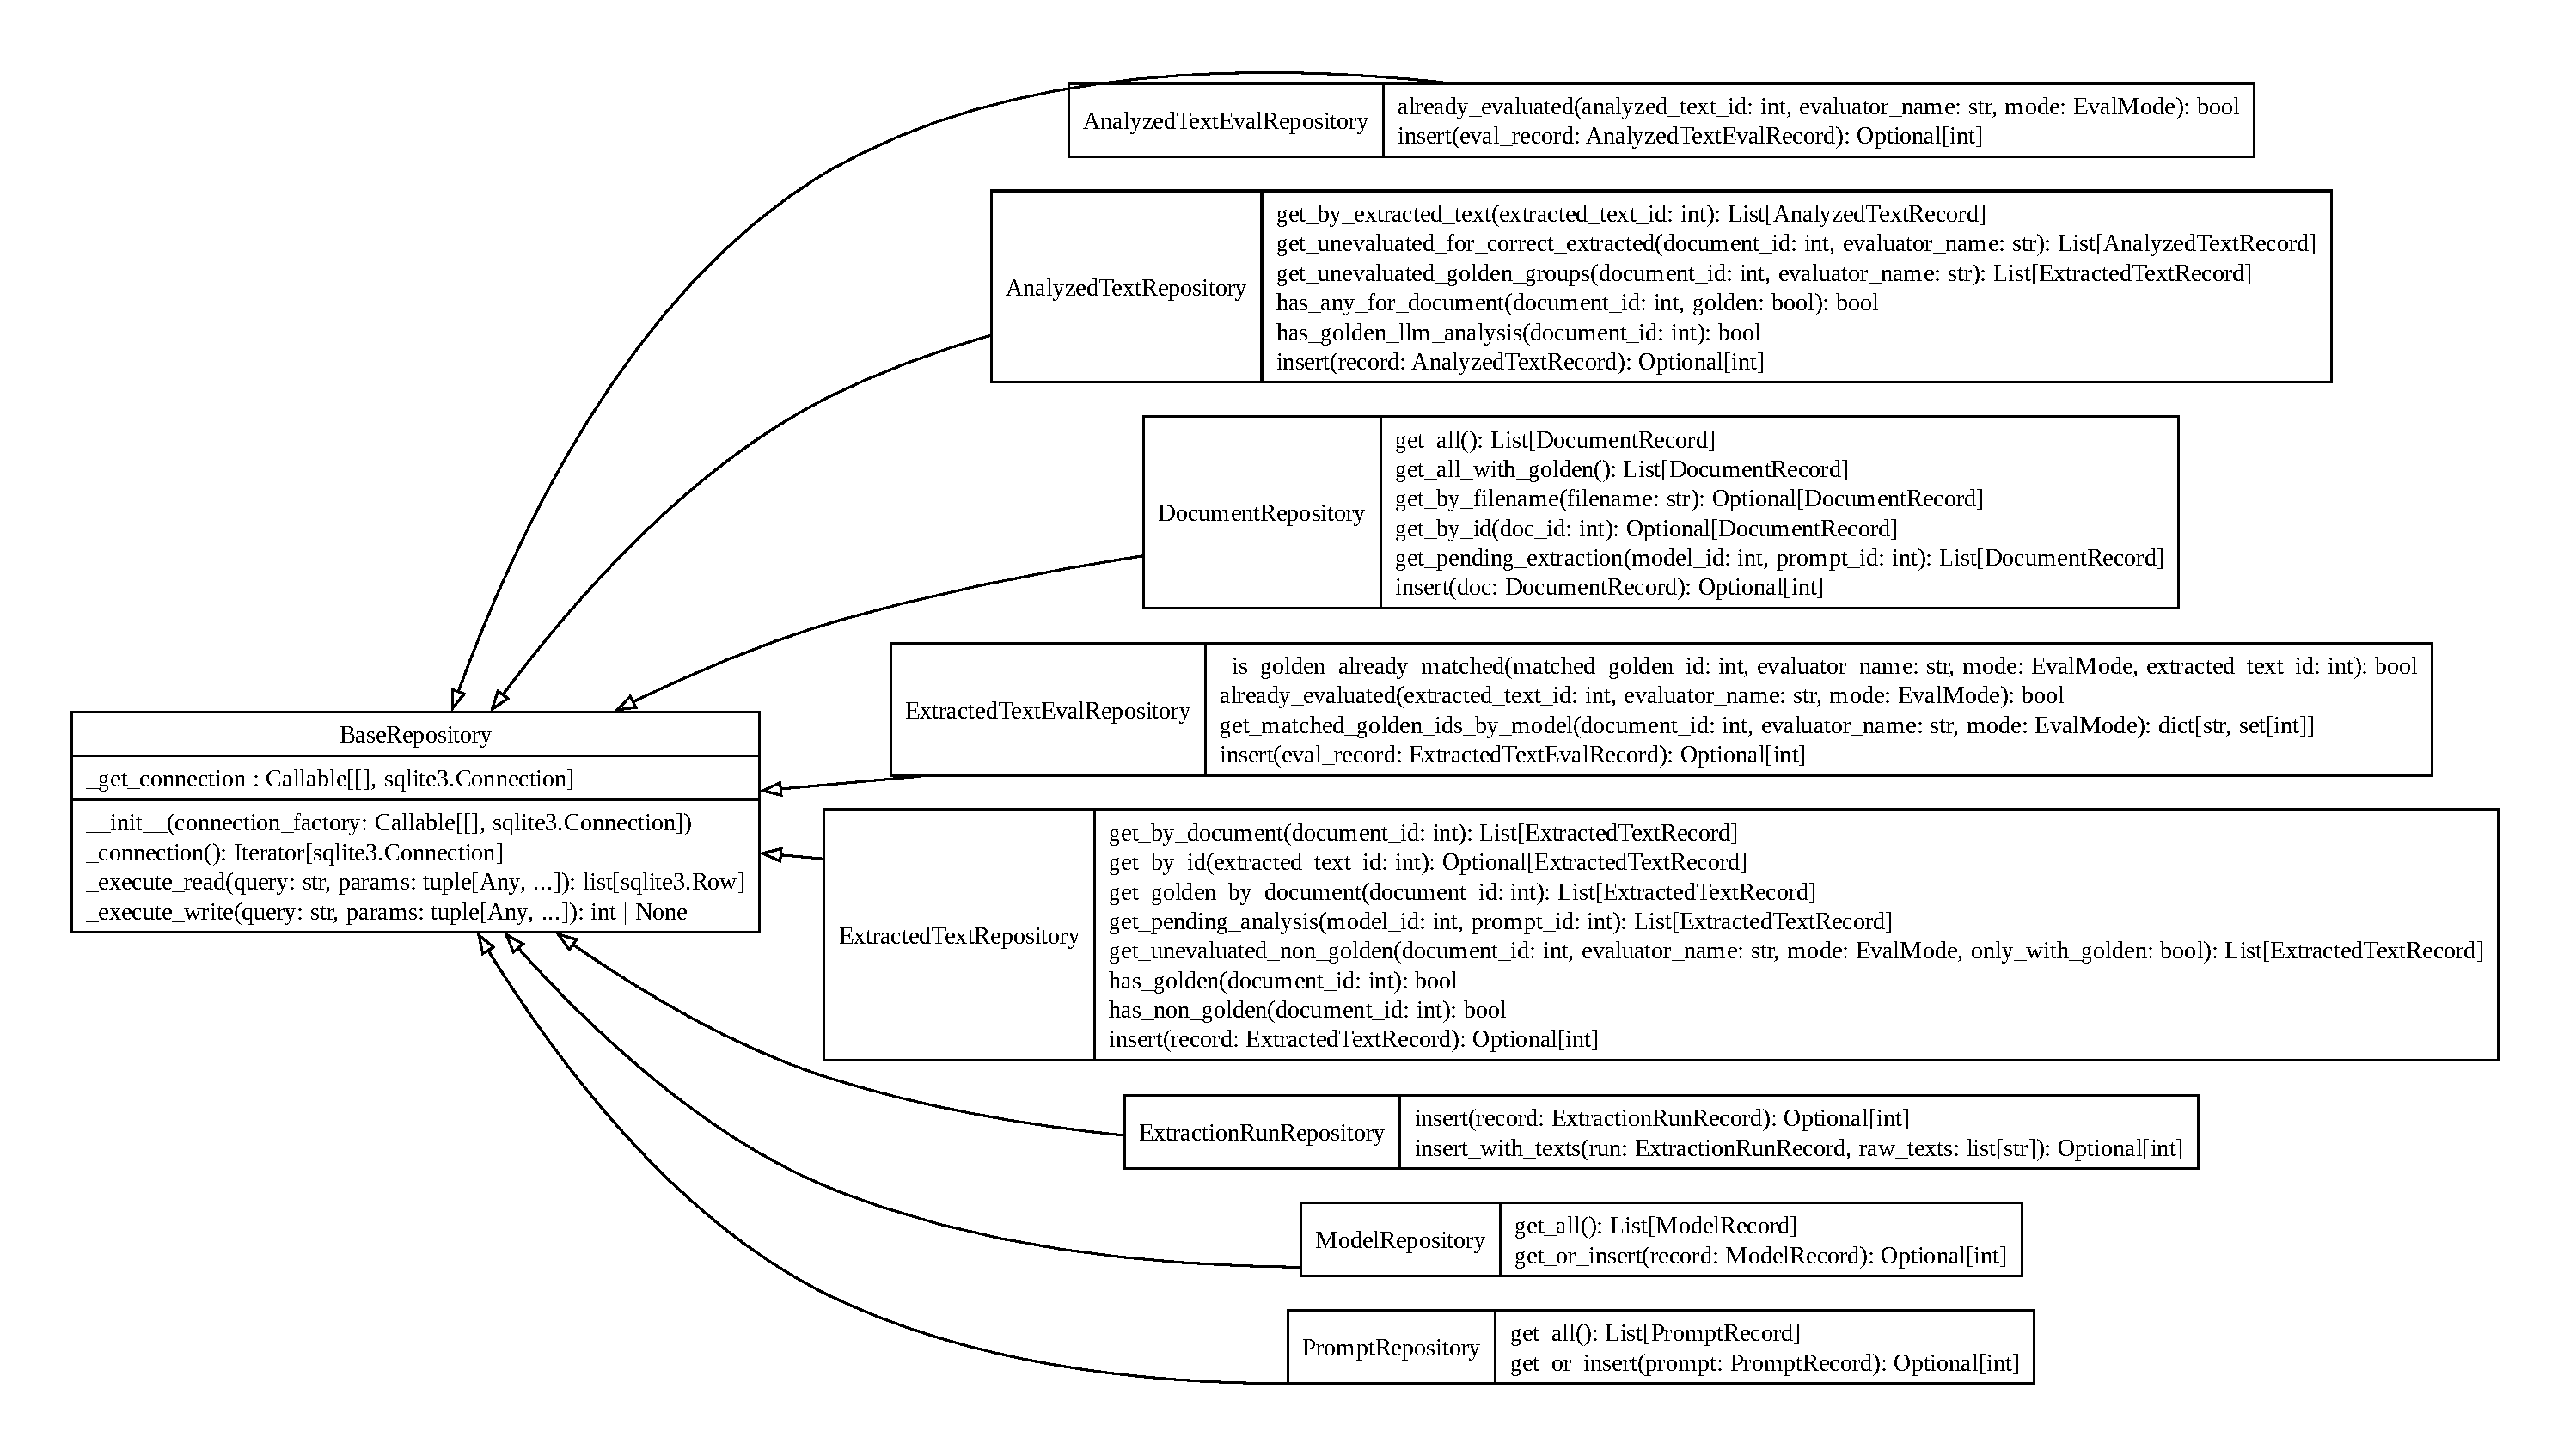
\includegraphics[width=0.9\linewidth, height=\textheight, keepaspectratio]{res/classes/cls_db.pdf}
        \caption{Diagram tříd databázových repozitářů}
        \label{fig:cls_db}
    \end{figure}
\end{landscape}

\chapter{Diagram tříd pro GUI}\label{pril:cls_gui}
Následující stránka obsahuje obrázek \ref{fig:cls_gui} diagramu tříd grafického uživatelského rozhraní Textractor Studio pro program Textractor.

\begin{landscape}
    \begin{figure}
        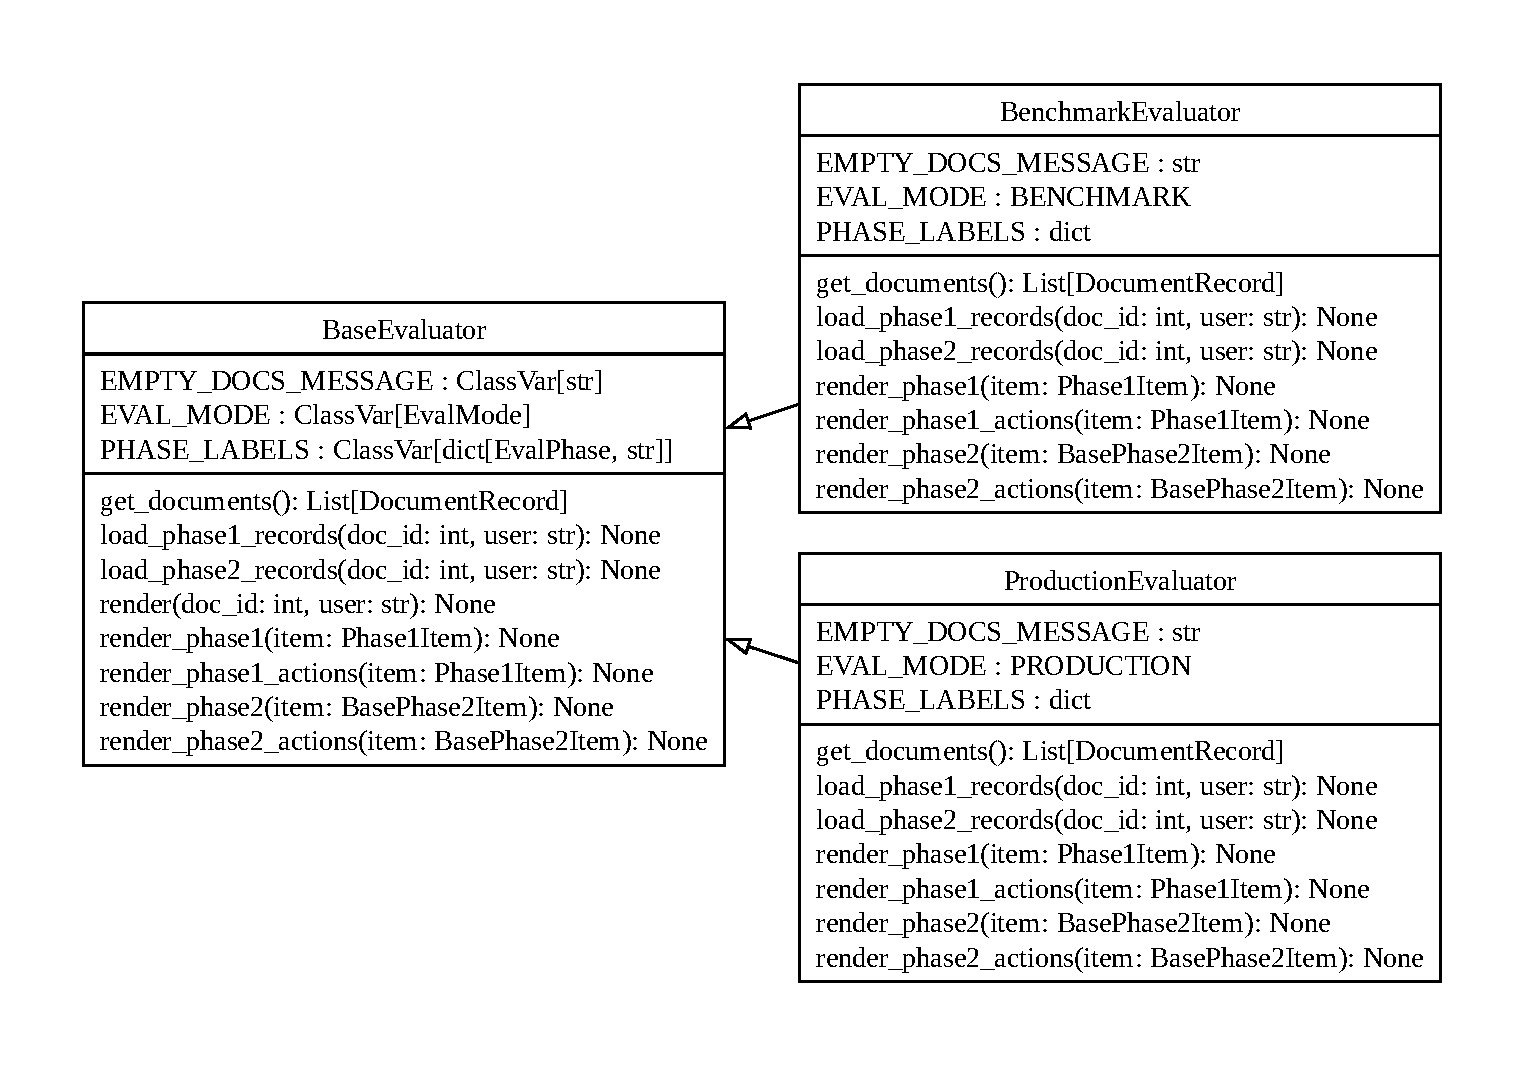
\includegraphics[width=\linewidth, height=\textheight, keepaspectratio]{res/classes/cls_gui.pdf}
    \caption{Diagram tříd pro grafické uživatelské rozhraní Textractor Studio}
    \label{fig:cls_gui}
    \end{figure}
\end{landscape}


\chapter{Uživatelská příručka pro spuštění programu Textractor}\label{sec:prirucka}
Tato uživatelská příručka informuje o~instalaci a spuštění programu Textractor na operačních systémech \product{Microsoft Windows} a \product{Linux}.

\section{Struktura archivu}
Archiv \filename"A23B0169P_prilohy.zip" obsahuje následující strukturu:
\begin{itemize}
    \item \filename"Aplikace_a_knihovny" -- její podsložka \filename"app/" obsahuje zdrojové soubory programu Textractor; podsložka \filename"docs/" obsahuje dokumentaci ke kódu programu ve formátu \verb"html" tvořenou knihovnou \product{pdoc} \cite{pdoc}.
    \item \filename"Text_prace" -- obsahuje zdrojové kódy k~dokumentu.
    \item \filename"Vstupni_data" -- její podložka \filename"raw_pdfs/" obsahuje dokumenty, na kterých bylo provedeno testování; podložka \filename"golden_seed/" obsahuje ručně extrahované a formalizované požadavky z~těchto dokumentů ve formátu \verb"json".
    \item \filename"Vysledky" -- databáze s~extrahovanými a formalizovanými požadavky a soubor se sestavou v~\product{Microsoft PowerBI} -- \filename"analyza_llm.pbix", kde probíhala analýza.
    \item \filename"Readme.txt" -- soubor s~informacemi o~spuštění a struktuře archivu.
\end{itemize}

\section{Minimální požadavky}
Spuštění aplikace bylo testováno na následujících technologiích:
\begin{itemize}
    \item Operační systém \product{Microsoft Windows} 11 nebo \product{Linux} (konkrétně \product{Fedora} verze 43).
    \item Interpreter jazyka \product{Python} verze 3.14.3.
    \item Správce balíčků pro \product{Python} -- \product{pip} verze 26.0.1.
    \item Virtuální prostředí pro \product{Python} -- \product{venv}.
\end{itemize}

\section{Instalace a spuštění}
Spuštění programu Textractor se dá docílit následujícími kroky:
\begin{enumerate}
    \item Stáhnout a rozbalit archiv \filename"A23B0169P_prilohy.zip".
    \item Přesunout se do kořenového adresáře programu Textractor v~\filename"Aplikace_a_knihovny/app".
    \item Spustit skript \command"setup.sh" (pro Linux, například pomocí příkazu \command"./setup.sh"), případně \command"setup.bat" (pro \product{Microsoft Windows}, například pomocí příkazu \command"setup.bat" nebo dvojím kliknutím). Obsah tohoto skriptu je popsán v~sekci \ref{sec:instalacni-skript}.
    \item Naplnění (případně vytvoření) souboru \filename".env" pro uložení proměnných do prostředí běhu, pokud není potřeba používat \textbf{jen Textractor Studio v~evaluačním režimu}. Pro tyto účely je vhodné upravit připravený soubor \filename"example.env".
    \item Nastavení virtuálního prostředí v~terminálu příkazem \\ \command"source .venv/bin/activate" (pro Linux), případně \command".venv\Source\activate" (pro \product{Microsoft Windows}).
    \item Spuštění samotného programu příkazem \command"python3 textractor.py", případně \command"py textractor.py" (pro \product{Microsoft Windows}).
    \item Po splnění předchozích kroků stačí následovat instrukce v~terminálu od programu Textractor.\footnote{V~případě nevyplnění potřebného API klíče je možné, že některé jazykové modely nebudou dostupné.}
\end{enumerate}

\subsection{Instalační skript}\label{sec:instalacni-skript}
Tento instalační skript vytvoří ve spouštěné složce (doporučeno spouštět v~kořenovém adresáři projektu) virtuální prostředí pro jazyk \product{Python}. Dále v~něm aktualizuje správce balíčků \product{pip}, pomocí kterého dalším příkazem nainstaluje potřebné knihovny pro běh programu:
\begin{itemize}
    \item \product{streamlit} verze 1.55.0,
    \item \product{streamlit\_pdf\_viewer} verze 0.0.28,
    \item \product{tqdm} verze 4.67.3,
    \item \product{typing\_extensions} verze 4.15.0,
    \item \product{python-dotenv} verze 1.2.2,
    \item \product{pydantic} verze 2.12.5,
    \item \product{pdfplumber} verze 0.11.9,
    \item \product{openai} verze 2.30.0,
    \item \product{mistralai} verze 2.1.3,
    \item \product{ollama} verze 0.6.1,
    \item \product{pypdfium2} verze 5.6.0.
\end{itemize}
Tyto knihovny a jejich verze se nachází v~souboru \filename"requirements.txt".

\subsection{Soubor s~proměnnými prostředí běhu}
Soubor \filename".env" obsahuje proměnné prostředí, kde s~některými program při běhu počítá a nelze ho bez nich spustit.

Hlavní proměnné jsou API klíče pro jazykové modely použité pro extrakční a formalizační fázi v~programu Textractor. Program počítá s~tím, že jsou použité pouze jazykové modely společností OpenAI (proměnná s~názvem \verb"OPENAI_API_KEY") a Mistral (proměnná s~názvem \verb"MISTRAL_API_KEY"). Případně lze použít lokální modely \product{Llama} od společnosti Meta, ovšem API klíč není potřeba.

Při použití rozhraní Textractor Studio, tedy pro evaluaci již extrahovaných požadavků tyto proměnné pro API klíče nejsou potřebné. Pro vyhodnocení je možné doplnit volitelnou proměnnou \verb"MODE", která označuje, zda se má Textractor Studio spustit v~produkčním nebo evaluačním režimu. Bez definování této proměnné se standardně \textbf{Textractor Studio} spustí v~evaluačním režimu. Pro produkční je nutné použít \verb"MODE=production" a pro evaluační režim \verb"MODE=benchmark".

Proměnná \verb"DATABASE_PATH" určuje cestu k~databázi, případně cestu, kde bude databáze vytvořena. Pokud není nastavena, použije se cesta \filename"data/database.db".

Výsledný soubor \filename".env" může vypadat například následovně:
\lstset{style=plain}
\begin{lstlisting}
OPENAI_API_KEY=api-klic-pro-openai
MISTRAL_API_KEY=api-klic-pro-mistral
DATABASE_PATH=data/database.db
MODE=benchmark
\end{lstlisting}



\chapter{Systémová zpráva u~extrakční fáze}\label{pril:system-message-extraction}

\lstset{style=plain}
\begin{lstlisting}
You are an expert Requirements Engineer analyzing Software Requirement Specifications (SRS).
Your task is to carefully read the provided document and extract EVERY explicitly stated project requirement, constraint, or goal.

RULES:
1. COPY the raw text exactly as it appears in the document. Do not summarize or rephrase. IMPORTANT: If the source text contains double quotes ("), you must replace them with single quotes (') to ensure valid JSON output.
2. If some text section contains full context required for understanding the requirement the section is about, you should COPY ALL PARTS CONTAINING THE REQUIREMENT. For example, if there is a table, you should copy whole table as it is. Another example, when there is a long text and somewhere inside it there is a requirement without context, you should copy the sentence and ADDITIONALLY ADD CONTEXT to it (section title, sentence related to requirement, ...) -- there is still rule, that the context should be COPY -- so do not modify the sentences.
3. Extract ALL requirements. Missing a requirement is a critical failure.
4. You MUST return a valid JSON object with the following structure: 
{
    "raw_text": [
        "requirement 1", 
        "requirement 2", 
        ...
    ]
}
\end{lstlisting}


\chapter{Systémová zpráva u~formalizační fáze}\label{pril:system-message-formalization}

\lstset{style=plain}
\begin{lstlisting}
You are an expert Technical Analyst. Your task is to process and analyze a raw software requirement and convert it into a structured, developer-friendly format.

You will receive a single raw requirement text. Review it carefully.
Your goal is to extract quantifiable parameters (if present) OR provide a clear, concise technical summary of the requirement. A~single input text may contain multiple requirements - split them if needed.

As example, from raw text "Display refresh rate should be 60 Hz, internet response should be 5 ms (minimum) and the system should be accessible only to authorized users.", you should extract requirements with following summaries and parameters:

{
  "parsed_requirements": [
    {
      "requirement_summary": "Display refresh rate",
      "parameters": [
        { "parameter_value": 60, "parameter_unit": "Hz" }
      ]
    },
    {
      "requirement_summary": "Internet response time",
      "parameters": [
        {
            "parameter_value": 5, 
            "parameter_unit": "ms (minimum)"
        }
      ]
    },
    {
      "requirement_summary": "Access restricted to authorized users only",
      "parameters": []
    }
  ]
}

If the raw text clearly describes the requirement, copy is enough. But if the raw text is vague, ambiguous or contains a lot of unnecessary information, provide a concise and clear summary in "requirement_summary". The summary should be descriptive enough for software engineers to understand the requirement without referring back to the original text. Keep the language of the input - if the input is in Czech, the output must be in Czech, and so on.
You MUST return a valid JSON object with the following structure:
{
  "parsed_requirements": [
    {
      "requirement_summary": "...", 
      "parameters": [
        {
          "parameter_value": ..., 
          "parameter_unit": "..."
        }
      ]
    }
  ]
}
\end{lstlisting}

% == BACK MATTER ==
\backmatter

% == BACK COVER ==
\setbackpageqrcode
\backpage
\end{document}